% Created 2021-03-15 一 15:12
% Intended LaTeX compiler: pdflatex
\documentclass[11pt]{article}
\usepackage[utf8]{inputenc}
\usepackage[T1]{fontenc}
\usepackage{graphicx}
\usepackage{grffile}
\usepackage{longtable}
\usepackage{wrapfig}
\usepackage{rotating}
\usepackage[normalem]{ulem}
\usepackage{amsmath}
\usepackage{textcomp}
\usepackage{amssymb}
\usepackage{capt-of}
\usepackage{hyperref}
%%%%%%%%%%%%%%%%%%%%%%%%%%%%%%%%%%%%%%
%% TIPS                                 %%
%%%%%%%%%%%%%%%%%%%%%%%%%%%%%%%%%%%%%%
% \substack{a\\b} for multiple lines text

\usepackage[utf8]{inputenc}

\usepackage[B1,T1]{fontenc}

% pdfplots will load xolor automatically without option
\usepackage[dvipsnames]{xcolor}
%%%%%%%%%%%%%%%%%%%%%%%%%%%%%%%%%%%%%%%
%% MATH related pacakge                  %%
%%%%%%%%%%%%%%%%%%%%%%%%%%%%%%%%%%%%%%%
% \usepackage{amsmath} mathtools loads the amsmath
\usepackage{amsmath}
\usepackage{mathtools}


\usepackage{amsthm}
\usepackage{amsbsy}

%\usepackage{commath}

\usepackage{amssymb}
\usepackage{mathrsfs}
%\usepackage{mathabx}
\usepackage{stmaryrd}
\usepackage{empheq}

%for \not\ll
\usepackage{centernot}

\usepackage{scalerel}
\usepackage{stackengine}
\usepackage{stackrel}

\usepackage{nicematrix}
\usepackage{tensor}
\usepackage{blkarray}
\usepackage{siunitx}
\usepackage[f]{esvect}

\usepackage{unicode-math}
\setmainfont{TeX Gyre Pagella}
% \setmathfont{STIX}
%\setmathfont{texgyrepagella-math.otf}
%\setmathfont{Libertinus Math}
\setmathfont{Latin Modern Math}

 
% \setmathfont[range={\smwhtdiamond,\enclosediamond,\varlrtriangle}]{Latin Modern Math}
 \setmathfont[range={\rightrightarrows,\twoheadrightarrow,\leftrightsquigarrow,\triangledown,\vartriangle}]{XITS Math}
 \setmathfont[range={\int,\setminus}]{Libertinus Math}
 \setmathfont[range={\mathalpha}]{TeX Gyre Pagella Math}
% unicode is not good at this!
%\let\nmodels\nvDash


%%%%%%%%%%%%%%%%%%%%%%%%%%%%%%%%%%%%%%%
%% TIKZ related packages                 %%
%%%%%%%%%%%%%%%%%%%%%%%%%%%%%%%%%%%%%%%

\usepackage{pgfplots}
\pgfplotsset{compat=1.15}
\usepackage{tikz}
\usepackage{tikz-cd}
\usepackage{tikz-qtree}

\usetikzlibrary{arrows,positioning,calc,fadings,decorations,matrix,decorations,shapes.misc}
%setting from geogebra
\definecolor{ccqqqq}{rgb}{0.8,0,0}


%%%%%%%%%%%%%%%%%%%%%%%%%%%%%%%%%%%%%%%
%% MISCLELLANEOUS packages               %%
%%%%%%%%%%%%%%%%%%%%%%%%%%%%%%%%%%%%%%%
\usepackage[most]{tcolorbox}
\usepackage{threeparttable}
\usepackage{tabularx}

\usepackage{enumitem}

% wrong with preview
\usepackage{subcaption}
\usepackage{caption}
% {\aunclfamily\Huge}
\usepackage{auncial}

\usepackage{float}

\usepackage{fancyhdr}

\usepackage{ifthen}
\usepackage{xargs}


\usepackage{imakeidx}
\usepackage{hyperref}
\usepackage{soul}


%\usepackage[xetex]{preview}
%%%%%%%%%%%%%%%%%%%%%%%%%%%%%%%%%%%%%%%
%% USEPACKAGES end                       %%
%%%%%%%%%%%%%%%%%%%%%%%%%%%%%%%%%%%%%%%

% \setlist{nosep}
% \numberwithin{equation}{subsection}
% \fancyhead{} % Clear the headers
% \renewcommand{\headrulewidth}{0pt} % Width of line at top of page
% \fancyhead[R]{\slshape\leftmark} % Mark right [R] of page with Chapter name [\leftmark]
% \pagestyle{fancy} % Set default style for all content pages (not TOC, etc)


% \newlength\shlength
% \newcommand\vect[2][0]{\setlength\shlength{#1pt}%
%   \stackengine{-5.6pt}{$#2$}{\smash{$\kern\shlength%
%     \stackengine{7.55pt}{$\mathchar"017E$}%
%       {\rule{\widthof{$#2$}}{.57pt}\kern.4pt}{O}{r}{F}{F}{L}\kern-\shlength$}}%
%       {O}{c}{F}{T}{S}}


\indexsetup{othercode=\small}
\makeindex[columns=2,options={-s /media/wu/file/stuuudy/notes/index_style.ist},intoc]
\makeatletter
\def\@idxitem{\par\hangindent 0pt}
\makeatother


%\newcounter{dummy} \numberwithin{dummy}{section}
\newtheorem{dummy}{dummy}[section]
\theoremstyle{definition}
\newtheorem{definition}[dummy]{Definition}
\theoremstyle{plain}
\newtheorem{corollary}[dummy]{Corollary}
\newtheorem{lemma}[dummy]{Lemma}
\newtheorem{proposition}[dummy]{Proposition}
\newtheorem{theorem}[dummy]{Theorem}
\theoremstyle{definition}
\newtheorem{examplle}{Example}[section]
\theoremstyle{remark}
\newtheorem*{remark}{Remark}
\newtheorem{exercise}{Exercise}[subsection]
\newtheorem{observation}{Observation}[section]


\newenvironment{claim}[1]{\par\noindent\textbf{Claim:}\space#1}{}

\makeatletter
\DeclareFontFamily{U}{tipa}{}
\DeclareFontShape{U}{tipa}{m}{n}{<->tipa10}{}
\newcommand{\arc@char}{{\usefont{U}{tipa}{m}{n}\symbol{62}}}%

\newcommand{\arc}[1]{\mathpalette\arc@arc{#1}}

\newcommand{\arc@arc}[2]{%
  \sbox0{$\m@th#1#2$}%
  \vbox{
    \hbox{\resizebox{\wd0}{\height}{\arc@char}}
    \nointerlineskip
    \box0
  }%
}
\makeatother

\setcounter{MaxMatrixCols}{20}
%%%%%%% ABS
\DeclarePairedDelimiter\abss{\lvert}{\rvert}%
\DeclarePairedDelimiter\normm{\lVert}{\rVert}%

% Swap the definition of \abs* and \norm*, so that \abs
% and \norm resizes the size of the brackets, and the
% starred version does not.
\makeatletter
\let\oldabs\abss
%\def\abs{\@ifstar{\oldabs}{\oldabs*}}
\newcommand{\abs}{\@ifstar{\oldabs}{\oldabs*}}
\newcommand{\norm}[1]{\left\lVert#1\right\rVert}
%\let\oldnorm\normm
%\def\norm{\@ifstar{\oldnorm}{\oldnorm*}}
%\renewcommand{norm}{\@ifstar{\oldnorm}{\oldnorm*}}
\makeatother

% \newcommand\what[1]{\ThisStyle{%
%     \setbox0=\hbox{$\SavedStyle#1$}%
%     \stackengine{-1.0\ht0+.5pt}{$\SavedStyle#1$}{%
%       \stretchto{\scaleto{\SavedStyle\mkern.15mu\char'136}{2.6\wd0}}{1.4\ht0}%
%     }{O}{c}{F}{T}{S}%
%   }
% }

% \newcommand\wtilde[1]{\ThisStyle{%
%     \setbox0=\hbox{$\SavedStyle#1$}%
%     \stackengine{-.1\LMpt}{$\SavedStyle#1$}{%
%       \stretchto{\scaleto{\SavedStyle\mkern.2mu\AC}{.5150\wd0}}{.6\ht0}%
%     }{O}{c}{F}{T}{S}%
%   }
% }

% \newcommand\wbar[1]{\ThisStyle{%
%     \setbox0=\hbox{$\SavedStyle#1$}%
%     \stackengine{.5pt+\LMpt}{$\SavedStyle#1$}{%
%       \rule{\wd0}{\dimexpr.3\LMpt+.3pt}%
%     }{O}{c}{F}{T}{S}%
%   }
% }

\newcommand{\bl}[1] {\boldsymbol{#1}}
\newcommand{\Wt}[1] {\stackrel{\sim}{\smash{#1}\rule{0pt}{1.1ex}}}
\newcommand{\wt}[1] {\widetilde{#1}}
\newcommand{\tf}[1] {\textbf{#1}}


%For boxed texts in align, use Aboxed{}
%otherwise use boxed{}

\DeclareMathSymbol{\widehatsym}{\mathord}{largesymbols}{"62}
\newcommand\lowerwidehatsym{%
  \text{\smash{\raisebox{-1.3ex}{%
    $\widehatsym$}}}}
\newcommand\fixwidehat[1]{%
  \mathchoice
    {\accentset{\displaystyle\lowerwidehatsym}{#1}}
    {\accentset{\textstyle\lowerwidehatsym}{#1}}
    {\accentset{\scriptstyle\lowerwidehatsym}{#1}}
    {\accentset{\scriptscriptstyle\lowerwidehatsym}{#1}}
  }


\newcommand{\cupdot}{\mathbin{\dot{\cup}}}
\newcommand{\bigcupdot}{\mathop{\dot{\bigcup}}}

\usepackage{graphicx}

\usepackage[toc,page]{appendix}

% text on arrow for xRightarrow
\makeatletter
%\newcommand{\xRightarrow}[2][]{\ext@arrow 0359\Rightarrowfill@{#1}{#2}}
\makeatother

% Arbitrary long arrow
\newcommand{\Rarrow}[1]{%
\parbox{#1}{\tikz{\draw[->](0,0)--(#1,0);}}
}

\newcommand{\LRarrow}[1]{%
\parbox{#1}{\tikz{\draw[<->](0,0)--(#1,0);}}
}


\makeatletter
\providecommand*{\rmodels}{%
  \mathrel{%
    \mathpalette\@rmodels\models
  }%
}
\newcommand*{\@rmodels}[2]{%
  \reflectbox{$\m@th#1#2$}%
}
\makeatother







\newcommand{\trcl}[1]{%
  \mathrm{trcl}{(#1)}
}



% Roman numerals
\makeatletter
\newcommand*{\rom}[1]{\expandafter\@slowromancap\romannumeral #1@}
\makeatother
% \\def \\b\([a-zA-Z]\) {\\boldsymbol{[a-zA-z]}}
% \\DeclareMathOperator{\\b\1}{\\textbf{\1}}


\DeclareMathOperator{\bx}{\textbf{x}}
\DeclareMathOperator{\bz}{\textbf{z}}
\DeclareMathOperator{\bff}{\textbf{f}}
\DeclareMathOperator{\ba}{\textbf{a}}
\DeclareMathOperator{\bk}{\textbf{k}}
\DeclareMathOperator{\bs}{\textbf{s}}
\DeclareMathOperator{\bh}{\textbf{h}}
\DeclareMathOperator{\bc}{\textbf{c}}
\DeclareMathOperator{\br}{\textbf{r}}
\DeclareMathOperator{\bi}{\textbf{i}}
\DeclareMathOperator{\bj}{\textbf{j}}
\DeclareMathOperator{\bn}{\textbf{n}}
\DeclareMathOperator{\be}{\textbf{e}}
\DeclareMathOperator{\bo}{\textbf{o}}
\DeclareMathOperator{\bU}{\textbf{U}}
\DeclareMathOperator{\bL}{\textbf{L}}
\DeclareMathOperator{\bV}{\textbf{V}}
\def \bzero {\mathbf{0}}
\def \btwo {\mathbf{2}}
\DeclareMathOperator{\bv}{\textbf{v}}
\DeclareMathOperator{\bp}{\textbf{p}}
\DeclareMathOperator{\bI}{\textbf{I}}
\DeclareMathOperator{\bM}{\textbf{M}}
\DeclareMathOperator{\bN}{\textbf{N}}
\DeclareMathOperator{\bK}{\textbf{K}}
\DeclareMathOperator{\bt}{\textbf{t}}
\DeclareMathOperator{\bb}{\textbf{b}}
\DeclareMathOperator{\bA}{\textbf{A}}
\DeclareMathOperator{\bX}{\textbf{X}}
\DeclareMathOperator{\bu}{\textbf{u}}
\DeclareMathOperator{\bS}{\textbf{S}}
\DeclareMathOperator{\bZ}{\textbf{Z}}
\DeclareMathOperator{\bJ}{\textbf{J}}
\DeclareMathOperator{\by}{\textbf{y}}
\DeclareMathOperator{\bw}{\textbf{w}}
\DeclareMathOperator{\bT}{\textbf{T}}
\DeclareMathOperator{\bF}{\textbf{F}}
\DeclareMathOperator{\bmm}{\textbf{m}}
\DeclareMathOperator{\bW}{\textbf{W}}
\DeclareMathOperator{\bR}{\textbf{R}}
\DeclareMathOperator{\bC}{\textbf{C}}
\DeclareMathOperator{\bD}{\textbf{D}}
\DeclareMathOperator{\bE}{\textbf{E}}
\DeclareMathOperator{\bQ}{\textbf{Q}}
\DeclareMathOperator{\bP}{\textbf{P}}
\DeclareMathOperator{\bY}{\textbf{Y}}
\DeclareMathOperator{\bH}{\textbf{H}}
\DeclareMathOperator{\bB}{\textbf{B}}
\DeclareMathOperator{\bG}{\textbf{G}}
\def \blambda {\symbf{\lambda}}
\def \boldeta {\symbf{\eta}}
\def \balpha {\symbf{\alpha}}
\def \bbeta {\symbf{\beta}}
\def \bgamma {\symbf{\gamma}}
\def \bxi {\symbf{\xi}}
\def \bLambda {\symbf{\Lambda}}
\def \bGamma {\symbf{\Gamma}}

\newcommand{\bto}{{\boldsymbol{\to}}}
\newcommand{\Ra}{\Rightarrow}
\newcommand\und[1]{\underline{#1}}
\newcommand\ove[1]{\overline{#1}}
\def \bPhi {\boldsymbol{\Phi}}
\def \btheta {\boldsymbol{\theta}}
\def \bTheta {\boldsymbol{\Theta}}
\def \bmu {\boldsymbol{\mu}}
\def \bphi {\boldsymbol{\phi}}
\def \bSigma {\boldsymbol{\Sigma}}
\def \lb {\left\{}
\def \rb {\right\}}
\def \la {\langle}
\def \ra {\rangle}
\def \caln {\mathcal{N}}
\def \dissum {\displaystyle\Sigma}
\def \dispro {\displaystyle\prod}
\def \E {\mathbb{E}}
\def \Q {\mathbb{Q}}
\def \N {\mathbb{N}}
\def \V {\mathbb{V}}
\def \R {\mathbb{R}}
\def \P {\mathbb{P}}
\def \A {\mathbb{A}}
\def \F {\mathbb{F}}
\def \Z {\mathbb{Z}}
\def \I {\mathbb{I}}
\def \C {\mathbb{C}}
\def \cala {\mathcal{A}}
\def \cale {\mathcal{E}}
\def \calb {\mathcal{B}}
\def \calq {\mathcal{Q}}
\def \calp {\mathcal{P}}
\def \cals {\mathcal{S}}
\def \calx {\mathcal{X}}
\def \caly {\mathcal{Y}}
\def \calg {\mathcal{G}}
\def \cald {\mathcal{D}}
\def \caln {\mathcal{N}}
\def \calr {\mathcal{R}}
\def \calt {\mathcal{T}}
\def \calm {\mathcal{M}}
\def \calw {\mathcal{W}}
\def \calc {\mathcal{C}}
\def \calv {\mathcal{V}}
\def \calf {\mathcal{F}}
\def \calk {\mathcal{K}}
\def \call {\mathcal{L}}
\def \calu {\mathcal{U}}
\def \calo {\mathcal{O}}
\def \calh {\mathcal{H}}
\def \cali {\mathcal{I}}

\def \bcup {\bigcup}

% set theory

\def \zfcc {\textbf{ZFC}^-}
\def \ac  {\textbf{AC}}
\def \gl  {\textbf{L }}
\def \gll {\textbf{L}}
\newcommand{\zfm}{$\textbf{ZF}^-$}

%\def \zfm {$\textbf{ZF}^-$}
\def \zfmm {\textbf{ZF}^-}
\def \wf {\textbf{WF }}
\def \on {\textbf{On }}
\def \cm {\textbf{M }}
\def \cn {\textbf{N }}
\def \cv {\textbf{V }}
\def \zc {\textbf{ZC }}
\def \zcm {\textbf{ZC}}
\def \zff {\textbf{ZF}}
\def \wfm {\textbf{WF}}
\def \onm {\textbf{On}}
\def \cmm {\textbf{M}}
\def \cnm {\textbf{N}}
\def \cvm {\textbf{V}}
\def \gchh {\textbf{GCH}}
\renewcommand{\restriction}{\mathord{\upharpoonright}}
\def \pred {\text{pred}}

\def \rank {\text{rank}}
\def \con {\text{Con}}
\def \deff {\text{Def}}


\def \uin {\underline{\in}}
\def \oin {\overline{\in}}
\def \uR {\underline{R}}
\def \oR {\overline{R}}
\def \uP {\underline{P}}
\def \oP {\overline{P}}

\def \dsum {\displaystyle\sum}

\def \Ra {\Rightarrow}

\def \e {\enspace}

\def \sgn {\operatorname{sgn}}
\def \gen {\operatorname{gen}}
\def \Hom {\operatorname{Hom}}
\def \hom {\operatorname{hom}}
\def \Sub {\operatorname{Sub}}

\def \supp {\operatorname{supp}}

\def \epiarrow {\twoheadarrow}
\def \monoarrow {\rightarrowtail}
\def \rrarrow {\rightrightarrows}

% \def \minus {\text{-}}
% \newcommand{\minus}{\scalebox{0.75}[1.0]{$-$}}
% \DeclareUnicodeCharacter{002D}{\minus}


\def \tril {\triangleleft}

\def \ACF {\text{ACF}}
\def \GL {\text{GL}}
\def \PGL {\text{PGL}}
\def \equal {=}
\def \deg {\text{deg}}
\def \degree {\text{degree}}
\def \app {\text{App}}
\def \FV {\text{FV}}
\def \conv {\text{conv}}
\def \cont {\text{cont}}
\DeclareMathOperator{\cl}{\textbf{CL}}
\DeclareMathOperator{\sg}{sg}
\DeclareMathOperator{\trdeg}{trdeg}
\def \Ord {\text{Ord}}

\DeclareMathOperator{\cf}{cf}
\DeclareMathOperator{\zfc}{ZFC}

%\DeclareMathOperator{\Th}{Th}
%\def \th {\text{Th}}
% \newcommand{\th}{\text{Th}}
\DeclareMathOperator{\type}{type}
\DeclareMathOperator{\zf}{\textbf{ZF}}
\def \fa {\mathfrak{a}}
\def \fb {\mathfrak{b}}
\def \fc {\mathfrak{c}}
\def \fd {\mathfrak{d}}
\def \fe {\mathfrak{e}}
\def \ff {\mathfrak{f}}
\def \fg {\mathfrak{g}}
\def \fh {\mathfrak{h}}
%\def \fi {\mathfrak{i}}
\def \fj {\mathfrak{j}}
\def \fk {\mathfrak{k}}
\def \fl {\mathfrak{l}}
\def \fm {\mathfrak{m}}
\def \fn {\mathfrak{n}}
\def \fo {\mathfrak{o}}
\def \fp {\mathfrak{p}}
\def \fq {\mathfrak{q}}
\def \fr {\mathfrak{r}}
\def \fs {\mathfrak{s}}
\def \ft {\mathfrak{t}}
\def \fu {\mathfrak{u}}
\def \fv {\mathfrak{v}}
\def \fw {\mathfrak{w}}
\def \fx {\mathfrak{x}}
\def \fy {\mathfrak{y}}
\def \fz {\mathfrak{z}}
\def \fA {\mathfrak{A}}
\def \fB {\mathfrak{B}}
\def \fC {\mathfrak{C}}
\def \fD {\mathfrak{D}}
\def \fE {\mathfrak{E}}
\def \fF {\mathfrak{F}}
\def \fG {\mathfrak{G}}
\def \fH {\mathfrak{H}}
\def \fI {\mathfrak{I}}
\def \fJ {\mathfrak{J}}
\def \fK {\mathfrak{K}}
\def \fL {\mathfrak{L}}
\def \fM {\mathfrak{M}}
\def \fN {\mathfrak{N}}
\def \fO {\mathfrak{O}}
\def \fP {\mathfrak{P}}
\def \fQ {\mathfrak{Q}}
\def \fR {\mathfrak{R}}
\def \fS {\mathfrak{S}}
\def \fT {\mathfrak{T}}
\def \fU {\mathfrak{U}}
\def \fV {\mathfrak{V}}
\def \fW {\mathfrak{W}}
\def \fX {\mathfrak{X}}
\def \fY {\mathfrak{Y}}
\def \fZ {\mathfrak{Z}}

\def \sfA {\textsf{A}}
\def \sfB {\textsf{B}}
\def \sfC {\textsf{C}}
\def \sfD {\textsf{D}}
\def \sfE {\textsf{E}}
\def \sfF {\textsf{F}}
\def \sfG {\textsf{G}}
\def \sfH {\textsf{H}}
\def \sfI {\textsf{I}}
\def \sfj {\textsf{J}}
\def \sfK {\textsf{K}}
\def \sfL {\textsf{L}}
\def \sfM {\textsf{M}}
\def \sfN {\textsf{N}}
\def \sfO {\textsf{O}}
\def \sfP {\textsf{P}}
\def \sfQ {\textsf{Q}}
\def \sfR {\textsf{R}}
\def \sfS {\textsf{S}}
\def \sfT {\textsf{T}}
\def \sfU {\textsf{U}}
\def \sfV {\textsf{V}}
\def \sfW {\textsf{W}}
\def \sfX {\textsf{X}}
\def \sfY {\textsf{Y}}
\def \sfZ {\textsf{Z}}
\def \sfa {\textsf{a}}
\def \sfb {\textsf{b}}
\def \sfc {\textsf{c}}
\def \sfd {\textsf{d}}
\def \sfe {\textsf{e}}
\def \sff {\textsf{f}}
\def \sfg {\textsf{g}}
\def \sfh {\textsf{h}}
\def \sfi {\textsf{i}}
\def \sfj {\textsf{j}}
\def \sfk {\textsf{k}}
\def \sfl {\textsf{l}}
\def \sfm {\textsf{m}}
\def \sfn {\textsf{n}}
\def \sfo {\textsf{o}}
\def \sfp {\textsf{p}}
\def \sfq {\textsf{q}}
\def \sfr {\textsf{r}}
\def \sfs {\textsf{s}}
\def \sft {\textsf{t}}
\def \sfu {\textsf{u}}
\def \sfv {\textsf{v}}
\def \sfw {\textsf{w}}
\def \sfx {\textsf{x}}
\def \sfy {\textsf{y}}
\def \sfz {\textsf{z}}



%\DeclareMathOperator{\ker}{ker}
\DeclareMathOperator{\im}{im}

\DeclareMathOperator{\inn}{Inn}
\DeclareMathOperator{\AC}{\textbf{AC}}
\DeclareMathOperator{\cod}{cod}
\DeclareMathOperator{\dom}{dom}
\DeclareMathOperator{\ran}{ran}
\DeclareMathOperator{\textd}{d}
\DeclareMathOperator{\td}{d}
\DeclareMathOperator{\id}{id}
\DeclareMathOperator{\LT}{LT}
\DeclareMathOperator{\Mat}{Mat}
\DeclareMathOperator{\Eq}{Eq}
\DeclareMathOperator{\irr}{irr}
\DeclareMathOperator{\Fr}{Fr}
\DeclareMathOperator{\Gal}{Gal}
\DeclareMathOperator{\lcm}{lcm}
\DeclareMathOperator{\alg}{\text{alg}}
\DeclareMathOperator{\Th}{Th}

\DeclareMathOperator{\DAG}{DAG}
\DeclareMathOperator{\ODAG}{ODAG}

% \varprod
\DeclareSymbolFont{largesymbolsA}{U}{txexa}{m}{n}
\DeclareMathSymbol{\varprod}{\mathop}{largesymbolsA}{16}
% \DeclareMathSymbol{\tonm}{\boldsymbol{\to}\textbf{Nm}}
\def \tonm {\bto\textbf{Nm}}
\def \tohm {\bto\textbf{Hm}}

% Category theory
\DeclareMathOperator{\Ab}{\textbf{Ab}}
\DeclareMathOperator{\Alg}{\textbf{Alg}}
\DeclareMathOperator{\Rng}{\textbf{Rng}}
\DeclareMathOperator{\Sets}{\textbf{Sets}}
\DeclareMathOperator{\Met}{\textbf{Met}}
\DeclareMathOperator{\BA}{\textbf{BA}}
\DeclareMathOperator{\Mon}{\textbf{Mon}}
\DeclareMathOperator{\Top}{\textbf{Top}}
\DeclareMathOperator{\Aut}{\textbf{Aut}}
\DeclareMathOperator{\RMod}{R-\textbf{Mod}}
\DeclareMathOperator{\RAlg}{R-\textbf{Alg}}
\DeclareMathOperator{\LF}{LF}
\DeclareMathOperator{\op}{op}
% Model theory
\DeclareMathOperator{\tp}{tp}
\DeclareMathOperator{\Diag}{Diag}
\DeclareMathOperator{\el}{el}
\DeclareMathOperator{\depth}{depth}
\DeclareMathOperator{\FO}{FO}
\DeclareMathOperator{\fin}{fin}
\DeclareMathOperator{\qr}{qr}
\DeclareMathOperator{\Mod}{Mod}
\DeclareMathOperator{\TC}{TC}
\DeclareMathOperator{\KH}{KH}
\DeclareMathOperator{\Part}{Part}
\DeclareMathOperator{\Infset}{\textsf{Infset}}
\DeclareMathOperator{\DLO}{\textsf{DLO}}
\DeclareMathOperator{\sfMod}{\textsf{Mod}}
\DeclareMathOperator{\AbG}{\textsf{AbG}}
\DeclareMathOperator{\sfACF}{\textsf{ACF}}
% Computability Theorem
\DeclareMathOperator{\Tot}{Tot}
\DeclareMathOperator{\graph}{graph}
\DeclareMathOperator{\Fin}{Fin}
\DeclareMathOperator{\Cof}{Cof}
\DeclareMathOperator{\lh}{lh}
% Commutative Algebra
\DeclareMathOperator{\ord}{ord}
\DeclareMathOperator{\Idem}{Idem}
\DeclareMathOperator{\zdiv}{z.div}
\DeclareMathOperator{\Frac}{Frac}
\DeclareMathOperator{\rad}{rad}
\DeclareMathOperator{\nil}{nil}
\DeclareMathOperator{\Ann}{Ann}
\DeclareMathOperator{\End}{End}
\DeclareMathOperator{\coim}{coim}
\DeclareMathOperator{\coker}{coker}
\DeclareMathOperator{\Bil}{Bil}
\DeclareMathOperator{\Tril}{Tril}
% Topology
\newcommand{\interior}[1]{%
  {\kern0pt#1}^{\mathrm{o}}%
}

% \makeatletter
% \newcommand{\vect}[1]{%
%   \vbox{\m@th \ialign {##\crcr
%   \vectfill\crcr\noalign{\kern-\p@ \nointerlineskip}
%   $\hfil\displaystyle{#1}\hfil$\crcr}}}
% \def\vectfill{%
%   $\m@th\smash-\mkern-7mu%
%   \cleaders\hbox{$\mkern-2mu\smash-\mkern-2mu$}\hfill
%   \mkern-7mu\raisebox{-3.81pt}[\p@][\p@]{$\mathord\mathchar"017E$}$}

% \newcommand{\amsvect}{%
%   \mathpalette {\overarrow@\vectfill@}}
% \def\vectfill@{\arrowfill@\relbar\relbar{\raisebox{-3.81pt}[\p@][\p@]{$\mathord\mathchar"017E$}}}

% \newcommand{\amsvectb}{%
% \newcommand{\vect}{%
%   \mathpalette {\overarrow@\vectfillb@}}
% \newcommand{\vecbar}{%
%   \scalebox{0.8}{$\relbar$}}
% \def\vectfillb@{\arrowfill@\vecbar\vecbar{\raisebox{-4.35pt}[\p@][\p@]{$\mathord\mathchar"017E$}}}
% \makeatother
% \bigtimes

\DeclareFontFamily{U}{mathx}{\hyphenchar\font45}
\DeclareFontShape{U}{mathx}{m}{n}{
      <5> <6> <7> <8> <9> <10>
      <10.95> <12> <14.4> <17.28> <20.74> <24.88>
      mathx10
      }{}
\DeclareSymbolFont{mathx}{U}{mathx}{m}{n}
\DeclareMathSymbol{\bigtimes}{1}{mathx}{"91}
% \odiv
\DeclareFontFamily{U}{matha}{\hyphenchar\font45}
\DeclareFontShape{U}{matha}{m}{n}{
      <5> <6> <7> <8> <9> <10> gen * matha
      <10.95> matha10 <12> <14.4> <17.28> <20.74> <24.88> matha12
      }{}
\DeclareSymbolFont{matha}{U}{matha}{m}{n}
\DeclareMathSymbol{\odiv}         {2}{matha}{"63}


\newcommand\subsetsim{\mathrel{%
  \ooalign{\raise0.2ex\hbox{\scalebox{0.9}{$\subset$}}\cr\hidewidth\raise-0.85ex\hbox{\scalebox{0.9}{$\sim$}}\hidewidth\cr}}}
\newcommand\simsubset{\mathrel{%
  \ooalign{\raise-0.2ex\hbox{\scalebox{0.9}{$\subset$}}\cr\hidewidth\raise0.75ex\hbox{\scalebox{0.9}{$\sim$}}\hidewidth\cr}}}

\newcommand\simsubsetsim{\mathrel{%
  \ooalign{\raise0ex\hbox{\scalebox{0.8}{$\subset$}}\cr\hidewidth\raise1ex\hbox{\scalebox{0.75}{$\sim$}}\hidewidth\cr\raise-0.95ex\hbox{\scalebox{0.8}{$\sim$}}\cr\hidewidth}}}
\newcommand{\stcomp}[1]{{#1}^{\mathsf{c}}}

\setlength{\baselineskip}{0.8in}

\stackMath
\newcommand\yrightarrow[2][]{\mathrel{%
  \setbox2=\hbox{\stackon{\scriptstyle#1}{\scriptstyle#2}}%
  \stackunder[0pt]{%
    \xrightarrow{\makebox[\dimexpr\wd2\relax]{$\scriptstyle#2$}}%
  }{%
   \scriptstyle#1\,%
  }%
}}
\newcommand\yleftarrow[2][]{\mathrel{%
  \setbox2=\hbox{\stackon{\scriptstyle#1}{\scriptstyle#2}}%
  \stackunder[0pt]{%
    \xleftarrow{\makebox[\dimexpr\wd2\relax]{$\scriptstyle#2$}}%
  }{%
   \scriptstyle#1\,%
  }%
}}
\newcommand\yRightarrow[2][]{\mathrel{%
  \setbox2=\hbox{\stackon{\scriptstyle#1}{\scriptstyle#2}}%
  \stackunder[0pt]{%
    \xRightarrow{\makebox[\dimexpr\wd2\relax]{$\scriptstyle#2$}}%
  }{%
   \scriptstyle#1\,%
  }%
}}
\newcommand\yLeftarrow[2][]{\mathrel{%
  \setbox2=\hbox{\stackon{\scriptstyle#1}{\scriptstyle#2}}%
  \stackunder[0pt]{%
    \xLeftarrow{\makebox[\dimexpr\wd2\relax]{$\scriptstyle#2$}}%
  }{%
   \scriptstyle#1\,%
  }%
}}

\newcommand\altxrightarrow[2][0pt]{\mathrel{\ensurestackMath{\stackengine%
  {\dimexpr#1-7.5pt}{\xrightarrow{\phantom{#2}}}{\scriptstyle\!#2\,}%
  {O}{c}{F}{F}{S}}}}
\newcommand\altxleftarrow[2][0pt]{\mathrel{\ensurestackMath{\stackengine%
  {\dimexpr#1-7.5pt}{\xleftarrow{\phantom{#2}}}{\scriptstyle\!#2\,}%
  {O}{c}{F}{F}{S}}}}

\newenvironment{bsm}{% % short for 'bracketed small matrix'
  \left[ \begin{smallmatrix} }{%
  \end{smallmatrix} \right]}

\newenvironment{psm}{% % short for ' small matrix'
  \left( \begin{smallmatrix} }{%
  \end{smallmatrix} \right)}

\newcommand{\bbar}[1]{\mkern 1.5mu\overline{\mkern-1.5mu#1\mkern-1.5mu}\mkern 1.5mu}

\newcommand{\bigzero}{\mbox{\normalfont\Large\bfseries 0}}
\newcommand{\rvline}{\hspace*{-\arraycolsep}\vline\hspace*{-\arraycolsep}}

\font\zallman=Zallman at 40pt
\font\elzevier=Elzevier at 40pt

\newcommand\isoto{\stackrel{\textstyle\sim}{\smash{\longrightarrow}\rule{0pt}{0.4ex}}}
\newcommand\embto{\stackrel{\textstyle\prec}{\smash{\longrightarrow}\rule{0pt}{0.4ex}}}

% from http://www.actual.world/resources/tex/doc/TikZ.pdf

\tikzset{
modal/.style={>=stealth’,shorten >=1pt,shorten <=1pt,auto,node distance=1.5cm,
semithick},
world/.style={circle,draw,minimum size=0.5cm,fill=gray!15},
point/.style={circle,draw,inner sep=0.5mm,fill=black},
reflexive above/.style={->,loop,looseness=7,in=120,out=60},
reflexive below/.style={->,loop,looseness=7,in=240,out=300},
reflexive left/.style={->,loop,looseness=7,in=150,out=210},
reflexive right/.style={->,loop,looseness=7,in=30,out=330}
}


\makeatletter
\newcommand*{\doublerightarrow}[2]{\mathrel{
  \settowidth{\@tempdima}{$\scriptstyle#1$}
  \settowidth{\@tempdimb}{$\scriptstyle#2$}
  \ifdim\@tempdimb>\@tempdima \@tempdima=\@tempdimb\fi
  \mathop{\vcenter{
    \offinterlineskip\ialign{\hbox to\dimexpr\@tempdima+1em{##}\cr
    \rightarrowfill\cr\noalign{\kern.5ex}
    \rightarrowfill\cr}}}\limits^{\!#1}_{\!#2}}}
\newcommand*{\triplerightarrow}[1]{\mathrel{
  \settowidth{\@tempdima}{$\scriptstyle#1$}
  \mathop{\vcenter{
    \offinterlineskip\ialign{\hbox to\dimexpr\@tempdima+1em{##}\cr
    \rightarrowfill\cr\noalign{\kern.5ex}
    \rightarrowfill\cr\noalign{\kern.5ex}
    \rightarrowfill\cr}}}\limits^{\!#1}}}
\makeatother

% $A\doublerightarrow{a}{bcdefgh}B$

% $A\triplerightarrow{d_0,d_1,d_2}B$


\graphicspath{{../images/ModalLogic}}
\newcommand{\ue}{\fu\fe}
\newcommand{\ua}{\und{a}}
\newcommand{\sfFr}{\sfF\sfr}
\newcommand{\PC}{\textbf{PC}}
\newcommand{\KL}{\textbf{KL}}
\newcommand{\KB}{\textbf{KB}}
\newcommand{\KD}{\textbf{KD}}
\newcommand{\KF}{\textbf{K4}}
\newcommand{\KtQ}{\textbf{K}_t\textbf{Q}}
\newcommand{\KtTho}{\textbf{K}_t\textbf{Tho}}
\newcommand{\KtThoM}{\textbf{K}_t\textbf{ThoM}}
\author{wugouzi}
\date{\today}
\title{Modal Logic}
\hypersetup{
 pdfauthor={wugouzi},
 pdftitle={Modal Logic},
 pdfkeywords={},
 pdfsubject={},
 pdfcreator={Emacs 27.1 (Org mode 9.3)}, 
 pdflang={English}}
\begin{document}

\maketitle
\tableofcontents

\section{Basic Concepts}
\label{sec:org0e1d4ac}
\subsection{Modal Languages}
\label{sec:org7986f54}
\begin{definition}[]
The \textbf{basic modal language} is defined using  a set of \textbf{proposition letters} \(\Phi\)
whose elements are usually denoted \(p,q,r\) and so on, and a unary modal
operator \(\lozenge\). The well-formed \textbf{formulas} \(\phi\) of the basic modal
language are given by the rule
\begin{equation*}
\phi:=p\mid\bot\mid\neg\phi\mid\psi\vee\phi\mid\lozenge\phi
\end{equation*}
\end{definition}

\(\fM,w\Vdash\phi\)
\begin{definition}[]
A \textbf{modal similarity type} is a pair \(\tau=(O,\rho)\) where \(O\) is a non-empty
set, and \(\rho\) is a function \(O\to\N\). The elements of \(O\) are called \textbf{modal
operators}; we use \(\triangle\), \(\triangle_0,\triangle_1,\dots\) to denote
elements of \(O\). The function \(\rho\) assigns to each operator \(\delta\in O\) a
finite \textbf{arity}
\end{definition}

\begin{definition}[]
A \textbf{modal language} \(ML(\tau,\Phi)\) is built up using a modal similarity type
\(\tau=(O,\rho)\) and a set of proposition letters \(\Phi\). The set \(Form(\tau,\Phi)\) of
\textbf{modal formulas} over \(\tau\) and \(\Phi\) is given by the rule
\begin{equation*}
\phi:=p\mid\bot\mid\neg\phi\mid\phi_1\vee\phi_2\mid\triangle(\phi_1,\dots,\phi_{\rho(\triangle)})
\end{equation*}
where \(p\) ranges over elements of \(\Phi\)
\end{definition}

\begin{definition}[]
For each \(\triangle\in O\) the \textbf{dual} \(\triangledown\) of \(\triangle\) is defined
as \(\triangledown(\phi_1,\dots,\phi_n):=\neg\triangle(\neg\phi_1,\dots,\neg\phi_n)\)
\end{definition}

\begin{examplle}[The Basic Temporal Language]
The basic temporal language is built using a set of unary operators \(O=\{\la
   F\ra,\la P\ra\}\). The intended interpretation of a formula \(\la F\ra\phi\)
is ' \(\phi\) will be true at some Future time' and the intended interpretation of
\(\la P\ra\phi\) is ' \(\phi\) was true at some Past time.' This language is called
the \textbf{basic temporal language}. Their duals are written as \(G\) and \(H\) ('it
is Going to be the case' and 'it always Has been the case')

Let's denote the converse of a relation \(R\) by \(R^\smallsmile\). We will
call a frame of the form \((T,R,R^\smallsmile)\) a \textbf{bidirectional frame}, and a
model built over such a frame a \textbf{bidirectional model}. From now on, we will
only interpret basic temporal language in bidirectional models. That is, if
\(\fM=(T,R,R^\smallsmile,V)\) is a bidirectional model then
\begin{align*}
\fM,t\Vdash F\phi \quad&\text{ iff }\quad
\exists s(Rts\wedge \fM,s\Vdash\phi)\\
\fM,t\Vdash P\phi \quad&\text{ iff }\quad
\exists s(R^\smallsmile ts\wedge \fM,s\Vdash\phi)
\end{align*}
\end{examplle}

\begin{examplle}[Propositional Dynamic Logic]
Each of these diamonds has the form \(\la\pi\ra\), where \(\pi\) denotes a
(non-deterministic) \textbf{program}. The intended interpretation of \(\la\pi\ra\) is
'some terminating execution of \(\pi\) from the present state leas to a state
bearing the information \(\phi\) '. The dual assertion \([\pi]\phi\) states that
'every execution of \(\pi\) from the present state leads to a state bearing the
information \(\phi\) '

Suppose we have fixed some set of basic programs \(a,b,c\) and so on. Then we
are allowed to define complex programs \(\pi\) over this base as follows
\begin{enumerate}
\item \textbf{Choice}. If \(\pi_1,\pi_2\) are programs, then so is \(\pi_1\cup\pi_2\)
\item \textbf{Composition}. so is \(\pi_1;\pi_2\)
\item \textbf{Iteration}. so is \(\pi^*\)
\end{enumerate}


This is called \textbf{regular} PDL. There are also
\begin{enumerate}
\item \textbf{Intersection} if \(\pi_1,\pi_2\) are programs, then so is
\(\pi_1\cap\pi_2\)

execute both \(\pi_1,\pi_2\), in parallel

\item \textbf{test} if \(\phi\) is a formula, then so is \(\phi?\)

test whether \(\phi\) holds, and if so, continues; if not, it fails
\end{enumerate}

The language of PDL has an infinite collection of diamonds, each indexed by a
program \(\pi\) build from basic programs using the constructor \(\cup,;\) and
\(^*\).
\begin{align*}
 &R_{\pi_1\cup\pi_2}=R_{\pi_1}\cup R_{\pi_2}\\
 &R_{\pi_1;\pi_2}=R_{\pi_1}\circ R_{\pi_2}\\
 &R_{\pi_1^*}=(R_{\pi_1})^*
 \end{align*}

Suppose  we have fixed a set of basic programs. Let \(\Pi\) be the set of programs
containing the basic programs and all the programs constructed over them
using the regular constructors \(\cup,;,^*\). Then a \textbf{regular frame for} \(\Pi\) is
a labeled transitive system \((W,\{R_\pi\mid\pi\in\Pi\})\) s..t \(R_a\) is an
arbitrary binary  relation for each basic program \(a\), and for all complex
programs \(\pi\), \(R_{\pi}\) is the binary relation inductively constructed in
accordance with the previous clauses. A \textbf{regular model} for \(\Pi\) is a model built
over a regular frame.
\end{examplle}

\begin{examplle}[An Arrow Language]
The type \(\tau_\to\) of \textbf{arrow logic} is a similarity type with modal
operators other than diamonds. The language of arrow logic is designed to
talk about the objects in arrow structures. The well-formed formulas \(\phi\) are
given by
\begin{equation*}
\phi:=p\mid\bot\mid\neg\phi\mid\phi\vee\psi\mid\phi\circ\psi\mid
\otimes\phi\mid 1'
\end{equation*}
1' ('identity') is a nullary modality, the 'converse' operator \(\otimes\) is
a diamond, and the 'composition' operator \(\circ\) is a dyadic operator.
Possible readings of these operators are:
\begin{alignat*}{3}
&1'&&\text{identity}&&\text{'skip'}\\
&\otimes\phi&&\text{converse}&&\text{'\(\phi\) conversely'}\\
&\phi\circ\psi\quad&&\text{composition}\quad&&\text{'first \(\phi\), then \(\psi\)'}
\end{alignat*}
\end{examplle}
\subsection{Models and Frames}
\label{sec:org7a9a602}
\begin{definition}[]
A \textbf{frame} for the basic modal language is a pair \(\fF=(W,R)\) s.t.
\begin{enumerate}
\item \(W\) is a non-empty set
\item \(R\) is a binary relation on \(W\)
\end{enumerate}


A \textbf{model} for the basic modal language is a pair \(\fM=(\fF,V)\), where \(\fF\)
is a frame for the basic modal language and \(V\) is a function assigning to
each proposition letter \(p\) in \(\Phi\) a subset \(V(p)\) of \(W\). The function
\(V\) is called a \textbf{valuation}. \(\fM\) is \textbf{based on} the frame \(\fF\)
\end{definition}

\begin{definition}[]
Suppose \(w\) is a state in a model \(\fM=(W,R,V)\). Then \(\phi\) is \textbf{satisfied} in
\(\fM\) at state \(w\) if
\begin{align*}
\fM,w\Vdash p&\quad\text{iff}\quad
w\in V(p),\text{ where } p\in\Phi\\
\fM,w\Vdash\bot&\quad\text{iff}\quad\text{never}\\
\fM,w\Vdash\neg\phi&\quad\text{iff}\quad
\text{not }\fM,w\Vdash\phi\\
\fM,w\Vdash\phi\vee\psi&\quad\text{iff}\quad
\fM,w\Vdash\phi\text{ or }\fM,w\Vdash\psi\\
\fM,w\Vdash\lozenge\phi&\quad\text{iff}\quad
\text{ for some }v\in W\text{ with }Rwv\text{ we have }\fM,v\Vdash\phi
\end{align*}
It follows that \(\fM,w\Vdash\Box\phi\) iff for all \(v\in W\) s.t.
\(Rwv\), we have \(\fM,v\Vdash\phi\)
\end{definition}

\begin{definition}[]
Let \(\tau\) be a modal similarity type. A \textbf{\(\tau\)-frame} is a tuple \(\fF\)
consisting of the following ingredients
\begin{enumerate}
\item a non-empty set \(W\)
\item for each \(n\ge0\), and each \(n\)-ary modal operator \(\triangle\) in the
similarity type \(\tau\), an \((n+1)\)-ary relation \(R_{\triangle}\)
\end{enumerate}
\end{definition}

\(\phi\) is \textbf{satisfied at a state \(w\)} in a model
\(\fM=(W,\{R_{\triangle}\mid\triangle\in\tau\},V)\) when
\(\rho(\triangle)\iffalse<\fi>0\) if
\begin{align*}
\fM,w\Vdash\triangle(\phi_1,\dots,\phi_n)\quad\text{iff}\quad&
\text{for some }v_1,\dots,v_n\in W\text{ with } R_{\triangle} wv_1\dots v_n\\
&\text{we have, for each }i,\fM,v_i\Vdash\phi_i
\end{align*}

When \(\rho(\triangle)=0\) we define
\begin{equation*}
\fM,w\Vdash\triangle \quad\text{ iff }\quad
w\in R_{\triangle}
\end{equation*}

\begin{definition}[]
The set of all formulas that are valid in a class of frames \(\sfF\)is called
the \textbf{logic} of \(\sfF\) (notation: \(\Lambda_{\sfF}\))
\end{definition}

\subsection{General Frames}
\label{sec:org709d269}

\begin{definition}[]
Given an \((n+1)\)-ary relation \(R\) on a set \(W\), we define the following
\(n\)-ary operation \(m_R\) on the power set \(\calp(W)\) of \(W\):
\begin{equation*}
m_R(X_1,\dots,X_n)=\{w\in W\mid Rww_1\dots w_n\text{ for some }
w_1\in X_1,\dots,w_n\in X_n\}
\end{equation*}
\end{definition}

\begin{definition}[General Frames]
Let \(\tau\) be a modal similarity type. A \textbf{general \(\tau\)-frame} is a pair
\((\fF,A)\) where \(\fF=(W,R_{\triangle})_{\triangle\in\tau}\) is a
\(\tau\)-frame, and \(A\) is a non-empty collection of \textbf{admissible} subsets of
\(W\) closed under following operations
\begin{enumerate}
\item union: if \(X,Y\in A\), then \(X\cup Y\in A\)
\item relative complement: if \(X\in A\), then \(W\setminus X\in A\)
\item modal operations: if \(X_1,\dots,X_n\in A\), then
\(m_{R_{\triangle}}(X_1,\dots,X_n)\in A\) for all \(\triangle\in\tau\)
\end{enumerate}


A \textbf{model based on a general frame} is a triple \((\fF,A,V)\) where \((\fF,A)\)
is a general frame and \(V\) is a valuation satisfying the constraint that
for each proposition letter \(p\), \(V(p)\) is an element of \(A\). Valuation
satisfying this constraint are called \textbf{admissible} for \((\fF,A)\)
\end{definition}

A set of admissible valuations \(A\) is a 'logically closed' collection of
information assignment

\begin{definition}[]
A formula \(\phi\) is \textbf{valid at a state \(w\) in a general frame} \((\fF,A)\)
(notation: \((\fF,A),w\Vdash\phi\))if \(\phi\) is true at \(w\) in every admissible
model \((\fF,A,V)\) on \((\fF,A)\); and \(\phi\) is \textbf{valid in a general frame}
\((\fF,A)\) (notation: \((\fF,A)\Vdash\phi\)) if \(\phi\) is true at every state in
every admissible model
\end{definition}



\subsection{Normal Modal Logics}
\label{sec:orgceccacf}
\begin{definition}[]
A \textbf{\(\bK\)-proof} is a finite sequence of formulas, each of which is an \textbf{axiom},
or follows from one or more earlier items in the sequence by applying a \textbf{rule
of proof}. The axioms of \(\bK\) are \textbf{all instances of propositional
tautologies} plus
\begin{alignat*}{2}
&\text{(K)}&&\Box(p\to q)\to(\Box p\to\Box q)\\
&\text{(Dual)}\quad&&\Diamond p\leftrightarrow\neg\Box\neg p
\end{alignat*}
The rules of proof of \(\bK\) are
\begin{itemize}
\item \textbf{Modus ponens}: given \(\phi\) and \(\phi\to\psi\) prove \(\psi\)
\item \textbf{Uniform substitution}: given \(\phi\), prove \(\theta\), where \(\theta\) is obtained from \(\phi\) by
uniformly replacing proposition letters in \(\phi\) by arbitrary formulas
\item \textbf{Generalization}: given \(\phi\), prove \(\Box\phi\)
\end{itemize}


A formula \(\phi\) is \textbf{\(\bK\)-provable} if it occurs as the last items of some
\(\bK\)-proof, and if this is the case we write \(\vdash_{\bK}\phi\)
\end{definition}

\begin{definition}[Normal Modal Logics]
A \textbf{normal modal logic} \(\Lambda\) is a set of formulas that contains all
tautologies, \(\Box(p\to q)\to(\Box p\to\Box q)\) and \(\Diamond
   p\leftrightarrow\neg\Box\neg p\), and that is closed under modus ponens,
uniform substitution and generalization. We call the smallest normal modal
logic \(\bK\)
\end{definition}

\subsection{Modal Consequence Relations}
\label{sec:orgacb370a}
\begin{definition}[Local Semantic Consequence]
Let \(\tau\) be a similarity type, and let \(\sfS\) be a class of structures of type
\(\tau\) (that is a class of models, a class of frames, or a class of general frames
of this type). Let \(\Sigma\) and \(\phi\) be a set of formulas and a single formula from a language of
type \(\tau\). We say that \(\phi\) is a \textbf{local semantic consequence of \(\Sigma\) over} \(\sfS\)
(notation: \(\Sigma\Vdash_{\sfS}\phi\)) if for all models \(\fM\) from
\(\sfS\), and all points \(w\) in \(\fM\), if \(\fM,w\Vdash\Sigma\) then \(\fM,w\Vdash\phi\)
\end{definition}

\begin{definition}[Global Semantic Consequence]
Let \(\tau,\sfS,\Sigma,\phi\). \(\phi\) is a \textbf{global semantic consequence of \(\Sigma\) over} \(\sfS\)
(notation \(\Sigma\Vdash_{\sfS}^g\phi\)) iff all structures \(\fG\in\sfS\),
if \(\fG\Vdash\Sigma\) then \(\fG\Vdash\phi\)
\end{definition}


\section{Models}
\label{sec:orgc4f0e45}
\subsection{Invariance Results}
\label{sec:orgca3b8eb}
\begin{definition}[]
Let \(\fM\) and \(\fM'\) be models of the same modal similarity type \(\tau\), and
let \(w\) and \(w'\) be states in \(\fM\) and \(\fM'\) respectively. The
\textbf{\(\tau\)-theory} (or \textbf{\(\tau\)-type}) \textbf{of} \(w\) is the set of all
\(\tau\)-formulas satisfied at \(w\): that is,
\(\{\phi\mid\fM,w\Vdash\phi\}\). We say that \(w\) and \(w'\) are \textbf{(modally)
equivalent} (\(w\leftrightsquigarrow w'\)) if they have the same \(\tau\)-theories

The \textbf{\(\tau\)-theory} of the model \(\fM\) is the set of all \(\tau\)-formulas
satisfied by all states in \(fM\); that is, \(\{\phi\mid\fM\Vdash\phi\}\)
Models \(\fM\) and \(\fM'\) are called
\textbf{(modally) equivalent} (\(\fM\leftrightsquigarrow\fM'\)) if their theories are identical
\end{definition}

\subsubsection{Disjoint Unions}
\label{sec:org224c543}
\subsubsection{Generated submodels}
\label{sec:orgdcfd290}
\begin{definition}[]
Let \(\fM=(W,R,V)\) and \(\fM'=(W',R',V')\) be two models; we say that
\(\fM'\) is a \textbf{submodel} of \(\fM\) if \(W'\subseteq W\), \(R'\) is the
restriction of \(R\) to \(W'\), and \(V'\) is the restriction of \(V\) to
\(\fM'\). We say that \(\fM'\) is a \textbf{generated submodel} of \(\fM\)
(\(\fM'\rightarrowtail\fM\)) if \(\fM'\) is a submodel of \(\fM\) and for
all points \(w\) the following closure condition holds
\begin{equation*}
\text{if }w\text{ is in }\fM'\text{ and }Rwv,\text{ then }v\text{ is in }\fM'
\end{equation*}

Let \(\fM\) be a model, and \(X\) a subset of the domain of \(\fM\); the
\textbf{submodel generated by} \(X\) is the smallest generated submodel of \(\fM\)
whose domain contains \(X\). A \textbf{rooted} or \textbf{point generated} model is a model
that is generated by a singleton set, the element of which is called the
\textbf{root} of the frame
\end{definition}

\subsubsection{Morphism for modalities}
\label{sec:org9752bb1}
\begin{definition}[Homomorphisms]
Let \(\tau\) be a modal similarity type and let \(\fM\) and \(\fM'\) be
\(\tau\)-models. By a \textbf{homomorphism} \(f:\fM\to\fM'\), we mean a function \(f:W\to
    W'\) satisfying
\begin{enumerate}
\item For each proposition letter \(p\) and each element \(w\) from \(\fM\), if
\(w\in V(p)\), then \(f(w)\in V'(p)\)
\item For each \(n\ge0\) and each \(n\)-ary \(\triangle\in\tau\) and
\((n+1)\)-tuple \(\bbar{w}\) from \(\fM\), if \((w_0,\dots,w_n)\in
       R_{\triangle}\), then \((f(w_0),\dots,f(w_n))\in R_{\triangle}'\) (the
\textbf{homomorphic condition})
\end{enumerate}
\end{definition}

\begin{definition}[Strong Homomorphisms, Embeddings and Isomorphisms]
Let \(\tau\) be a modal similarity type and let \(\fM\) and \(\fM'\) be
\(\tau\)-models. By a \textbf{strong homomorphism} \(f:\fM\to\fM'\), we mean a function \(f:W\to
    W'\) satisfying
\begin{enumerate}
\item For each proposition letter \(p\) and each element \(w\) from \(\fM\) iff
\(w\in V(p)\), then \(f(w)\in V'(p)\)
\item For each \(n\ge0\) and each \(n\)-ary \(\triangle\in\tau\) and
\((n+1)\)-tuple \(\bbar{w}\) from \(\fM\) iff \((w_0,\dots,w_n)\in
       R_{\triangle}\), iff \((f(w_0),\dots,f(w_n))\in R_{\triangle}'\) (the
\textbf{strong homomorphic condition})
\end{enumerate}


An \textbf{embedding} of \(\fM\) into \(\fM'\) is a strong homomorphism
\(f:\fM\to\fM'\) which is injective. An \textbf{isomorphism} is a bijective strong homomorphism
\end{definition}

\begin{proposition}[]
Let \(\tau\) be a modal similarity type and let \(\fM\) and \(\fM'\) be
\(\tau\)-models. Then the following holds
\begin{enumerate}
\item for all elements \(w\) and \(w'\) of \(\fM\) and \(\fM'\), respectively,
if there exists a surjective strong homomorphism \(f:\fM\to\fM'\) with
\(f(w)=w'\), then \(w\) and \(w\) are modally equivalent
\item If \(\fM\cong\fM'\), then \(\fM\leftrightsquigarrow\fM'\)
\end{enumerate}
\end{proposition}

\begin{definition}[Bounded Morphisms - the Basic Case]
Let \(\fM\) and \(\fM'\) be models for the basic modal language. A mapping
\(f:\fM=(W,R,V)\to\fM'=(W',R',V')\) is a \textbf{bounded morphsim} if it satisfies
\begin{enumerate}
\item \(w\) and \(f(w)\) satisfy the same proposition letters
\item \(f\) is a homomorphism w.r.t. the relation \(R\) (if \(Rwv\) then \(R'f(w)f(v)\))
\item If \(R'f(w)v'\) then there exists \(v\) s.t. \(Rwv\) and \(f(v)=v'\) (the
\textbf{back condition})
\end{enumerate}


If there is a \textbf{surjective} bounded morphism from \(\fM\) to \(\fM'\), then we
say that \(\fM'\) is a \textbf{bounded morphic image} of \(\fM\), and write
\(\fM\twoheadrightarrow\fM'\)
\end{definition}

\begin{proposition}[]
Let \(\tau\) be a modal similarity type and let \(\fM\) and \(\fM'\) be
\(\tau\)-models s.t. \(f:\fM\to\fM'\) is a bounded morphism. Then for each
modal formula \(\phi\), and each element \(w\) of \(\fM\) we have
\(\fM,w\Vdash\phi\) iff \(\fM',f(w)\Vdash\phi\).
\end{proposition}


Let \(\tau\) be a modal similarity type containing only diamonds (thus if \(\fM\)
is a \(\tau\)-model, it has the form \((W,R_1,\dots,V)\) where each \(R_i\)
is a binary relation on \(W\)) . In this context we will call a
\(\tau\)-model \(\fM\) \textbf{tree-like} if the structure \((W,\bigcup_i R_i,V)\) is
a tree

\begin{proposition}[]
\label{prop2.15}
Assume that \(\tau\) is a modal similarity type containing only diamonds. Then for
any rooted \(\tau\)-models \(\fM\) there exists a tree-like \(\tau\)-models
\(\fM'\) s.t. \(\fM'\twoheadrightarrow\fM\). Hence any satisfiable
\(\tau\)-formula is satisfiable in a tree-like model
\end{proposition}

\begin{proof}
Let \(w\) be the root of \(\fM\). Define the model \(\fM'\) as follows. Its
domain \(W'\) consist of all finite sequences \((w,u_1,\dots,u_n)\) s.t.
\(n\ge0\) and for some modal operators \(\la a_1\ra,\dots,\la
    a_n\ra\in\tau\) there is a path \(wR_{a_1}u_1\cdots R_{a_n}u_n\) in \(\fM\).
Define \((w,u_1,\dots,u_n)R'_a(w,v_1,\dots,w_m)\) to hold if
\(m=n+1,u_i=v_i\) for \(i=1,\dots,n\) and \(R_au_nv_m\) holds in \(\fM\).
That is, \(R'_a\) relates two sequences iff the second is an extension of
the first with a state from \(\fM\) that is a sucessor of the last element
of the first sequence. Finally, \(V'\) is defined by putting
\((w,u_1,\dots,u_n)\in V'(p)\) iff \(u_n\in V(p)\). The mapping
\(f:(w,u_1,\dots,u_n)\mapsto u_n\) defines a surjective bounded morphism
from \(\fM'\) to \(\fM\)
\end{proof}




\subsection{Bisimulations}
\label{sec:org0cfa15a}
\begin{definition}[Bisimulation - the Basic Case]
\label{def2.16}
Let \(\fM=(W,R,V)\) and \(\fM=(W',R',V')\) be two models

A non-empty binary relation \(Z\subseteq W\times W'\) is called a \textbf{bisimulation
between} \(\fM\) and \(\fM'\) (notation: \(Z:\fM\leftrightarroweq\fM')\) if
\begin{enumerate}
\item If \(wZw'\) then \(w\) and \(w'\) satisfy the same proposition letters
\item If \(wZw'\) and \(Rwv\), then there exists \(v'\) (in \(\fM'\)) s.t.
\(vZv'\) and \(R'w'v'\) (the \textbf{forth condition})
\item The converse of (2): if \(wZw'\) and \(R'w'v'\), then there exists \(v\)
(in \(\fM\)) s.t. \(vZv'\) and \(Rwv\) (the \textbf{back condition})
\end{enumerate}


When \(Z\) is a bisimulation linking two states \(w\) in \(\fM\) and \(w'\)
in \(\fM'\) we say that \(w\) and \(w'\) are \textbf{bisimilar}, and we write
\(Z:\fM,w\leftrightarroweq \fM',w'\). If there is a bisimulation, we sometimes
write \(\fM,w\leftrightarroweq \fM',w'\) or \(w\leftrightarroweq w'\)
\end{definition}

\begin{definition}[Bisimulation - the General Case]
Let \(\tau\) be a modal similarity type, and let
\(\fM=(W,R_{\triangle},V)_{\triangle\in\tau}\) and
\(\fM'=(W',R_{\triangle}',V')_{\triangle\in\tau}\) be \(\tau\)-models. A
non-empty binary relation \(Z\subseteq W\times W'\) is called a \textbf{bisimulation}
between \(\fM\) and \(\fM'\) (\(Z:\fM\leftrightarroweq\fM'\)) if the above
condition 1 is satisfied and
\begin{enumerate}
\setcounter{enumi}{1}
\item If \(wZw'\) and \(R_{\triangle}wv_1\dots v_n\) then there are
\(v_1',\dots,v_n'\in W'\) s.t. \(R'_{\triangle}w'v_1'\dots v_n'\) and for
all \(i\) (\(1\le i\le n\)) \(v_iZv_i'\) (the \textbf{forth} condition)
\item If \(wZw'\) and \(R'_{\triangle}w'v_1'\dots v_n'\) then there are
\(v_1,\dots,v_n\in W\) s.t. \(R_{\triangle}wv_1\dots v_n\) and for
all \(i\) (\(1\le i\le n\)) \(v_iZv_i'\) (the \textbf{back} condition)
\end{enumerate}
\end{definition}

\begin{proposition}[]
Let \(\tau\) be a modal similarity type, and let \(\fM,\fM'\) and \(\fM_i\) (\(i\in
   I\)) be \(\tau\)-models
\begin{enumerate}
\item If \(\fM\cong\fM'\), then \(\fM\leftrightarroweq\fM'\)
\item For every \(i\in I\), and every \(w\) in \(\fM_i\),
\(\fM_i,w\leftrightarroweq\biguplus_i\fM_i,w\)
\item If \(\fM'\rightarrowtail\fM\), then \(\fM',w\leftrightarroweq\fM,w\) for
all \(w\) in \(\fM'\)
\item If \(f:\fM\twoheadrightarrow\fM'\), then
\(\fM,w\leftrightarroweq\fM',f(w)\) for all \(w\) in \(\fM\)
\end{enumerate}
\end{proposition}

\begin{proof}
Suppose \(\fM=(W,R_{\triangle},V)_{\triangle\in\tau}\) and
\(\fM'=(W',R_{\triangle}',V')_{\triangle\in\tau}\) 
\(\fM_i\subseteq \biguplus_i\fM_i\)
\begin{enumerate}
\item Suppose \(f:\fM\cong\fM'\), then we define \(wZw'\) iff \(w'=f(w)\) where
\(w\in W,w'\in W'\). Bisimulation comes from the definition of the isomorphism
\item Define the relation \(Z=\{(w,w)\mid
      w\in\fM_i\}\subseteq\fM_i\times\biguplus\fM_i\). The first condition comes
from the invariance. The forth condition is obvious. For the back
condition, if \(R_{\triangle}'w'v_1'\dots v_n'\) and \(w'\in W\), then
\(v_1',\dots,v_n'\in W\) since each \(R_{\triangle,i}\) is disjoint and we
have \(R_{\triangle,i}w'v_1'\dots v_n'\)
\item Define the relation \(Z=\{(w,w)\mid w\in\fM'\}\subseteq\fM'\times\fM\).
The first condition comes from the invariance. Forth condition is obvious.
For the back condition, suppose \(wZw\) and \(R'_{\triangle}wv_1'\dots
      v_n'\), by the definition, \(v_1',\dots,v_n'\in W\) and
\(R_{\triangle}wv_1'\dots v_n'\)
\item Define \(Z=\{(w,f(w)\mid w\in W)\}\). The first condition comes from the
definition. If \(wZw'\) and \(R_{\triangle}wv_1\dots v_n\), then
\(R'_{\triangle}f(w)f(v_1)\dots f(v_n)\). If \(wZw'\) and
\(R_{\triangle}'w'v_1'\dots v_n\), then there is \(v_1,\dots,v_n\) s.t.
\(R_{\triangle}wv_1,\dots,v_n\) and \(f(v_i)=v_i'\) for \(1\le i\le n\)
\end{enumerate}
\end{proof}

\begin{theorem}[]
\label{thm2.20}
Let \(\tau\) be a modal similarity type, and let \(\fM, \fM'\) be \(\tau\)-models.
Then, for every \(w\in W\) and \(w'\in W'\), \(w\leftrightarroweq w'\)
implies that \(w\leftrightsquigarrow w'\). In other words, modal formulas are
invariant under bisimulation
\end{theorem}

\begin{proof}
Induction on the complexity of \(\phi\).

Suppose \(\phi\) is \(\diamond\psi\), we have \(\fM,w\Vdash\diamond\psi\) iff there
exists a \(v\) in \(\fM\) s.t. \(Rwv\) and \(\fM,v\Vdash\psi\). As
\(w\leftrightarroweq w'\), there exists a \(v'\) in \(\fM'\) s.t. \(R'w'v'\)
and \(v\leftrightarroweq v'\). By the I.H., \(\fM',v'\Vdash\psi\), hence \(\fM',w'\Vdash\diamond\psi\)
\end{proof}

\begin{examplle}[Bisimulation and First-Order Logic]
\label{example2.22}

\begin{center}
\includegraphics[width=.9\linewidth]{/media/wu/file/stuuudy/notes/images/ModalLogic/BisimilarModels.png}
\end{center}
\end{examplle}

\begin{examplle}[]
\label{example2.23}

\begin{center}
\includegraphics[width=.9\linewidth]{/media/wu/file/stuuudy/notes/images/ModalLogic/NotBisimilar.png}
\end{center}
\end{examplle}

\(\fM\) is \textbf{image-finite} if for each state \(u\) in \(\fM\) and each relation
\(R\) in \(\fM\), the set \(\{(v_1,\dots,v_n)\mid Ruv_1\dots v_n\}\) is
finite

\begin{theorem}[Hennessy-Milner Theorem]
\label{thm2.24}
Let \(\tau\) be a modal similarity type and let \(\fM\) and \(\fM'\) be two
image-finite \(\tau\)-models. Then for every \(w\in W\) and \(w'\in W'\),
\(w\leftrightarroweq w'\) iff \(w\leftrightsquigarrow w'\)
\end{theorem}

\begin{proof}
Assume that our similarity type \(\tau\) only contains a single diamond. The
direction from left to right follows from Theorem \ref{thm2.20}

Suppose \(w\leftrightsquigarrow w'\). The first condition is immediate. If
\(Rwv\), assume there is no \(v'\) in \(\fM'\) with \(R'w'v'\) and
\(v\leftrightsquigarrow v'\). Let \(S'=\{u'\mid R'w'u'\}\). Note that \(S'\)
must be non-empty, for otherwise \(\fM',w'\Vdash\Box\bot\), which would
contradict \(w\leftrightsquigarrow w'\) since \(\fM,w\Vdash\diamond\top\).
Furthermore, as \(\fM'\) is image-finite, \(S'\) must be finite, say
\(S'=\{w_1',\dots,w_n'\}\). By assumption, for every \(w_i'\in S'\) there
exists a formula \(\psi_i\) s.t. \(\fM,v\Vdash\psi_i\), but
\(\fM',w_i'\not\Vdash\psi_i\). It follows that
\begin{equation*}
\fM,w\Vdash\diamond(\psi_1\wedge\dots\wedge\psi_n)\quad\text{ and }\quad
\fM',w'\not\Vdash\diamond(\psi_1\wedge\dots\wedge \psi_n)
\end{equation*}
\end{proof}

\begin{exercise}
\label{ex2.2.8}
Suppose that \(\{Z_i\mid i\in I\}\) is a non-empty collection of
bisimulations between \(\fM\) and \(\fM'\). Prove that the relation
\(\bigcup_{i\in I}Z_i\) is also a bisimulation between \(\fM\) and \(\fM'\).
Conclude that if \(\fM\) and \(\fM'\) are bisimilar, then there is a maximal
bisimulation between \(\fM\) and \(\fM'\).
\end{exercise}

\begin{proof}
\begin{enumerate}
\item If \((w,w')\in\bigcup_{i\in I}Z_i\), then \((w,w')\in Z_j\) for some
\(j\in I\) and hence they satisfy the same propositional letters
\item If \((w,w')\in\bigcup_{i\in I}Z_i\) and \(R_{\triangle}wv_1\dots v_n\),
since \((w,w')\in Z_j\) for some \(j\in I\), we have
\(R'_{\triangle}w'v_1'\dots v_n'\) and \(v_iZ_jv_i'\) for all \(1\le i\le
      n\), which means \((v_i,v_i')\in\bigcup_{i\in I}Z_i\) for all \(1\le i\le n\)
\item similarly
\end{enumerate}
\end{proof}

\begin{remark}[Bisimulations for the Basic Temporal Language and Arrow Logic]
When working with the basic temporal language, we usually work with models
\((W,R,V)\) and implicitly take \(R_p\) to be \(R^\smallsmile\). Thus we need
a notion of bisimulation between models \((W,R,V)\) and \((W',R',V')\) to be
a relation \(Z\) between the states of the two models that satisfies the
clauses of Definition \ref{def2.16}, and in addition the following
\begin{enumerate}
\setcounter{enumi}{3}
\item If \(wZw'\) and \(Rvw\), then there exists \(v'\) in \(\fM'\) s.t.
\(vZv'\) and \(R'v'w'\)
\item Converse of 4: if \(wZw'\) and \(R'v'w'\), then there exists \(v\) in
\(\fM\) s.t. \(vZv'\)
\end{enumerate}
\end{remark}

\subsection{Finite Models}
\label{sec:orgc3992c8}
\begin{definition}[Finite Model Property]
Let \(\tau\) be a modal similarity type, and let \(\sfM\) be a class of
\(\tau\)-models. We say that \(\tau\) has the \textbf{finite model property w.r.t.} \(\sfM\)
if the following holds: if \(\phi\) is a formula of similarity type \(\tau\), and \(\phi\) is
satisfiable in some model in \(\sfM\), then \(\phi\) is satisfiable in a \textbf{finite}
model in \(\sfM\)
\end{definition}
\subsubsection{Selecting a finite submodel}
\label{sec:orgad0fff1}
\begin{definition}[Degree]
We define the \textbf{degree} of modal formulas as follows:
\begin{align*}
\deg(p)\quad&=\quad 0\\
\deg(\bot)\quad&=\quad0\\
\deg(\neg\phi)\quad&=\quad\deg(\phi)\\
\deg(\phi\vee\psi)\quad&=\quad\max\{\deg(\phi),\deg(\psi)\}\\
\deg(\triangle(\phi_1,\dots,\phi_n))\quad&=\quad
1+\max\{\deg(\phi_1),\dots,\deg(\phi_2)\}
\end{align*}
\end{definition}

\begin{proposition}[]
\label{prop2.29}
Let \(\tau\) be a finite modal similarity type, and assume our collection of
proposition letters is finite as well
\begin{enumerate}
\item for all \(n\), up to logical equivalence there are only finitely many
formulas of degree at most \(n\)
\item for all \(n\), and every \(\tau\)-model \(\fM\) and state \(w\) of
\(\fM\), the set of all \(\tau\)-formulas of degree at most \(n\) that
are satisfied by \(w\), is equivalent to a single formula
\end{enumerate}
\end{proposition}

\begin{definition}[$n$-Bisimulation]
Let \(\fM\) and \(\fM'\) be models, and let \(w\) and \(w'\) be states of
\(\fM\) and \(\fM'\), respectively. We say that \(w\) and \(w'\) are
\textbf{\(n\)-bisimilar} (\(w\leftrightarroweq_nw'\)) if there exists a sequence of
binary relations \(Z_n\subseteq\cdots\subseteq Z_0\) with the following
properties (for \(i+1\le n\))
\begin{enumerate}
\item \(wZ_nw'\)
\item if \(vZ_0v'\) then \(v\) and \(v'\) agree on all proposition letters
\item if \(vZ_{i+1}v'\) and \(Rvu\) then there exists \(u'\) with \(R'v'u'\)
and \(uZ_iu'\)
\item if \(vZ_{i+1}v'\) and \(R'v'u'\), then there exists \(u\) with \(Rvu\)
and \(uZ_iu'\)
\end{enumerate}
\end{definition}

\begin{proposition}[]
\label{prop2.31}
Let \(\tau\) be a finite modal similarity type, \(\Phi\) a finite set of proposition
letters, and let \(\fM\) and \(\fM'\) be models for this language. Then for
every \(w\) in \(\fM\) and \(w'\) in \(\fM'\), the following are equivalent
\begin{enumerate}
\item \(w\leftrightarroweq_nw'\)
\item \(w\) and \(w'\) agree on all modal formulas of degree at most \(n\).
\end{enumerate}
\end{proposition}

\begin{proof}
\(2\to 1\). if \(n=0\), obvious.

If \(n=k\) and the proposition holds. Now suppose \(n=k+1\). Now \(w\) and
\(w'\) agree on all modal formulas of degree at most \(n+1\). If
there is not \(v,v'\) s.t. \(v\) and \(v'\) agree on all modal formulas of
degree at most \(n\) and \(Rwv\) and \(Rwv'\). Let \(S'=\{u'\mid R'w'u'\}\)
and \(S'\) is finite, say \(S'==\{w_1',\dots,w_n'\}\). By assumption, for
every \(w_i'\in S'\) there exists a formula \(\psi_i\)  of degree at most
\(n\) s.t. \(\fM,v\Vdash\psi_i\) but \(\fM',w_i'\not\Vdash\psi_i\). It
follows that
\begin{equation*}
\fM,w\Vdash\diamond(\psi_1\wedge\dots\wedge\psi_n)
\text{ and }
\fM',w'\not\Vdash\diamond(\psi_1\wedge\dots\wedge\psi_n)
\end{equation*}
\end{proof}

\begin{definition}[]
Let \(\tau\) be a modal similarity type containing only diamonds. Let
\(\fM=(W,R_1,\dots,R_n,\dots,V)\) be a rooted \(\tau\)-model with root
\(w\). The notion of the \textbf{height} of states in \(\fM\) is defined by
induction.

The only element of height 0 is the rot of the model; the states of height
\(n+1\) are those immediate successors of elements of height \(n\) that have
not yet assigned a height smaller than \(n+1\). The \textbf{height of a model} \(\fM\)
is the maximum \(n\) s.t. there is a state of height \(n\) in \(\fM\), if
such a maximum exists; otherwise the height of \(\fM\) is infinite

For a natural number \(k\), the \textbf{restriction} of \(\fM\) to \(k\)
(\(\fM\restriction k\)) is defined as the submodel containing only states
whose height is at most \(k\). \((\fM\restriction
    k)=(W_k,R_{1k},\dots,R_{nk},\dots,V_k)\), where
\(W_k=\{v\mid\text{height}(v)\le k\}\), \(R_{nk}=R_n\cap(W_k\times W_k)\),
and for each \(p\), \(V_k(p)=V(p)\cap W_k\)
\end{definition}


\begin{lemma}[]
\label{lemma2.33}
Let \(\tau\) be a modal similarity type that contains only diamonds. Let \(\fM\) be
a rooted \(\tau\)-models, and let \(k\) be a natural number. Then for every
state \(w\) of \((\fM\restriction k)\), we have \((\fM\restriction
    k),w\leftrightarroweq_l\fM,w\), where \(l=k-\text{height}(w)\)
\end{lemma}

\begin{theorem}[Finite Model Property - via Selection]
Let \(\tau\) be a modal similarity type containing only diamonds, and let \(\phi\) be a
\(\tau\)-formula. If \(\phi\) is satisfiable, then it is satisfiable on a finite model
\end{theorem}

\begin{proof}
Fix a modal formula \(\phi\) with \(\deg(\phi)=k\). We restrict our modal similarity
type \(\tau\) and our collection of proposition letters to the modal operators and
proposition letters actually occurring in \(\phi\). Let \(\fM_1,w_1\) be s.t.
\(\fM_1,w_1\Vdash\phi\). By Proposition \ref{prop2.15}, there exists a
tree-like model \(\fM_2\) with root \(w_2\) s.t. \(\fM_2,w_2\Vdash\phi\).
Let \(\fM_3:=(\fM_2\restriction k)\). By Lemma \ref{lemma2.33} we have
\(\fM_2,w_2\leftrightarroweq_k\fM_3,w_2\) and by Proposition \ref{prop2.31} it
follows that \(\fM_3,w_2\Vdash\phi\)

By induction on \(n\le k\) we define finite sets of states \(S_0,\dots,S_k\)
and a (final) model \(\fM_4\) with domain \(S_0\cup\cdots\cup S_k\); the
points in each \(S_n\) will have height \(n\)

Define \(S_0\) to be the singleton \(\{w_2\}\). Next, assume that
\(S_0,\dots,S_n\) have already been defined. Fix an element \(v\) of
\(S_n\). By Proposition \ref{prop2.29} there are only finitely many
non-equivalent modal formulas whose degree is at most \(k-n\), say
\(\psi_1,\dots,\psi_m\). For each formula that is of the form \(\la
    a\ra\chi\) and holds in \(\fM_3\) at \(v\), select a state \(u\) from
\(\fM_3\) s.t. \(R_avu\) and \(\fM_3,u\Vdash\chi\). Add all these \(u\)s to
\(S_{n+1}\), and repeat this selection process for every state in \(S_n\).
\(S_{n+1}\) is defined as the set of all points that have been selected in
this way

Finally, define \(\fM_4\) as follows. Its domain is \(S_0\cup\dots\cup
    S_k\); as each \(S_i\) is finite, \(\fM_4\) is finite. The relations and
valuation are obtained by restricting the relations and valuations of
\(\fM_3\) to the domain of \(\fM_4\)
\end{proof}
\subsubsection{Finite models via filtrations}
\label{sec:org9deca5e}

\begin{definition}[]
A set of formulas \(\Sigma\) is \textbf{closed under subformulas} (or \textbf{subformula closed}) if
for all formulas \(\phi\), \(\phi'\): if \(\phi\vee\phi'\in\Sigma\) then so are
\(\phi\) and \(\phi'\); if \(\neg\phi\in\Sigma\) then so is \(\phi\); and if
\(\triangle(\phi_1,\dots,\phi_n)\in\Sigma\) then so are \(\phi_1,\dots,\phi_n\)
\end{definition}

\begin{definition}[Filtrations]
We work in the basic modal language. Let \(\fM=(W,R,V)\) be a model and \(\Sigma\) a
subformula closed set of formulas. Let \(\leftrightsquigarrow_\Sigma\) be
the relation on the states of \(\fM\) defined by
\begin{equation*}
w\leftrightsquigarrow_\Sigma v \text{ iff for all }\phi\in\Sigma:
(\fM,w\Vdash\phi\text{ iff }\fM,v\Vdash\phi)
\end{equation*}
Note that \(\leftrightsquigarrow_\Sigma\) is an equivalence relation. We
denote the equivalence class of a state \(w\) of \(\fM\) w.r.t.
\(\leftrightsquigarrow_\Sigma\) by \(\abs{w}_\Sigma\), or simply
\(\abs{w}\). The mapping \(w\mapsto\abs{w}\) is called the \textbf{natural map}

Let \(W_\Sigma=\{\abs{w}_\Sigma\mid w\in W\}\). Suppose \(\fM_\Sigma^f\) is
any model \((W^f,R^f,V^f)\) s.t.
\begin{enumerate}
\item \(W^f=W_\Sigma\)
\item if \(Rwv\) then \(R^f\abs{w}\abs{v}\)
\item if \(R^f\abs{w}\abs{v}\) then for all \(\diamond\phi\in\Sigma\), if
\(\fM,v\Vdash\phi\) then \(\fM,w\Vdash\diamond\phi\)
\item \(V^f(p)=\{\abs{w}\mid\fM,w\Vdash p\}\), for all proposition letters
\(p\) in \(\Sigma\)
\end{enumerate}


\(\fM_\Sigma^f\) is called a \textbf{filtration of \(\fM\) through} \(\Sigma\); we will
often suppress subscripts and write \(\fM^f\) instead of \(\fM_\Sigma^f\)
\end{definition}
\label{def2.36}
\begin{center}
\includegraphics[width=6cm]{/media/wu/file/stuuudy/notes/images/ModalLogic/Filtration.png}
\end{center}

Let \(\fM=(\N,R,V)\) , where \(R=\{(0,1),(0,2),(1,3)\}\cup\{(n,n+1)\mid
    n\ge2\}\), and \(V\) has \(V(p)=\N\setminus\{0\}\) and \(V(q)=\{2\}\)

Further assume \(\Sigma=\{\diamond p,p\}\). \(\Sigma\) is subformula closed. Then,
the model
\(\fN=(\{\abs{0},\abs{1}\},\{(\abs{0},\abs{1}),(\abs{1},\abs{1})\},V')\),
where \(V'(p)=\{\abs{1}\}\) is a filtration of \(\fM\) through \(\Sigma\). \(\fN\) is
not a bounded morphic image of \(\fM\): any bounded morphism would have to
preserve the formula \(q\)

\begin{proposition}[]
Let \(\Sigma\) be a finite subformula closed set of basic modal formulas. For any
model \(\fM\), if \(\fM^f\) is a filtration of \(\fM\) through a subformula
closed set \(\Sigma\), then \(\fM^f\) contains at most \(2^n\) nodes (where \(n\)
denotes the size of \(\Sigma\))
\end{proposition}

\begin{proof}
The states of \(\fM^f\) are the equivalence classes in \(W_\Sigma\). Let
\(g\) be the function with domain \(W_\Sigma\) and range \(\calp(\Sigma)\)
defined by \(g(\abs{w})=\{\phi\in\Sigma\mid\fM,w\Vdash\phi\}\). It follows
from the definition of \(\leftrightsquigarrow_\Sigma\) that \(g\) is well
defined and injective. Thus \(\abs{W_\Sigma}\le 2^n,n=\abs{\Sigma}\)
\end{proof}

\begin{theorem}[Filtration Theorem]
\label{thm2.39}
Consider the basic modal language. Let \(\fM^f=(W_\Sigma,R^f,V^f)\) be a
filtration of \(\fM\) through a subformula closed set \(\Sigma\). Then for all
formulas \(\phi\in\Sigma\), and all nodes \(w\) in \(\fM\), we have
\(\fM,w\Vdash\phi\) iff \(\fM^f,\abs{w}\Vdash\phi\)
\end{theorem}

\begin{proof}
Suppose \(\diamond\phi\in\Sigma\) and \(\fM,w\Vdash\diamond\phi\). Then there
is a \(v\) s.t. \(Rwv\) and \(\fM,v\Vdash\phi\). As \(\fM^f\) is a
filtration, \(R^f\abs{w}\abs{v}\). As \(\Sigma\) is a subformula closed,
\(\phi\in\Sigma\), thus by the inductive hypothesis
\(\fM^f,\abs{v}\Vdash\phi\). Hence \(\fM^f,\abs\Vdash\diamond\phi\)

Suppose \(\diamond\phi\in\Sigma\) and \(\fM^f,\abs{w}\Vdash\diamond\phi\).
Thus there is a state \(\abs{v}\) in \(\fM^f\) s.t. \(R^f\abs{w}\abs{v}\)
and \(\fM^f,\abs{v}\Vdash\phi\). As \(\phi\in\Sigma\), we have
\(\fM,v\Vdash\phi\). By the definition, we have \(\fM,w\Vdash\diamond\phi\)
\end{proof}

Note that clauses 2 and 3 of Definition \ref{def2.36} are designed to make the
modal case of the inductive step go through.

Define
\begin{enumerate}
\item \(R^s\abs{w}\abs{v}\) iff \(\exists w'\in\abs{w}\exists v'\in\abs{v}Rw'v'\)
\item \(R^l\abs{w}\abs{v}\) iff for all formulas \(\diamond\phi\in\Sigma\):
\(\fM,v\Vdash\phi\) implies \(\fM,w\Vdash\diamond\phi\)
\end{enumerate}


These relations give rise to the \textbf{smallest} and \textbf{largest} filtrations respectively

\begin{lemma}[]
Consider the basic modal language. Let \(\fM\) be any model, \(\Sigma\) any
subformula closed set of formulas, \(W_\Sigma\) the set of equivalence
classes induced by \(\leftrightsquigarrow_\Sigma\), and \(V^f\) the standard
valuation on \(W_\Sigma\). Then both \((W_\Sigma,R^s,V^f)\) and
\((W_\Sigma,R^l,V^f)\) are filtrations of \(\fM\) through \(\Sigma\). Furthermore, if
\((W_\Sigma, R^f,V^f)\) is any filtration of \(\fM\) through \(\Sigma\), then
\(R^s\subseteq R^f\subseteq R^l\)
\end{lemma}

\begin{proof}
If \(Rwv\), if \(\fM,v\Vdash\phi\), then \(\fM,w\Vdash\diamond\phi\), hence
\(R^l\abs{w}\abs{v}\)

For any \((W_\Sigma,R^f,V^f)\). \(R^s\subseteq R^f\) by clause 2.
\(R^f\subseteq R^l\) by clause 2
\end{proof}

\begin{theorem}[Finite Model Property - via Filtrations]
Let \(\phi\) be a basic modal formula. if \(\phi\) is satisfiable, then it is satisfiable
on a finite model. Indeed, it is satisfiable on a finite model containing at
most \(2^m\) nodes, where \(m\) is the number of subformulas of \(\phi\)
\end{theorem}

\begin{proof}
Assume that \(\phi\) is satisfiable on a model \(\fM\); take any filtration of
\(\fM\) through the set of subformulas .
\end{proof}

\begin{lemma}[]
Let \(\fM\) be a model, \(\Sigma\) a subformula closed set of formulas, and
\(W_\Sigma\) the set of equivalence classes induced on \(\fM\) by
\(\leftrightsquigarrow_\Sigma\). Let \(R^t\) be the binary relation on
\(W_\Sigma\) defined by
\begin{equation*}
R^t\abs{w}\abs{v} \text{ iff for all }\phi, \text{ if }\diamond\phi\in\Sigma
\text{ and }\fM,v\Vdash\phi\vee\diamond\phi\text{ then }\fM,w\Vdash\diamond\phi
\end{equation*}
If \(R\) is transitive then \((W_\Sigma,R^t,V^f)\) is a filtration and
\(R^t\) is transitive
\end{lemma}

\begin{definition}[]
Let \((W,R,V)\) be a transitive frame. A \textbf{cluster} on \((W,R,V)\) is a
maximal, nonempty equivalence class under \(R\). That is, \(C\subseteq W\)
is a cluster if the restriction of \(R\) to \(C\) is an equivalence relation

A cluster is \textbf{simple} if it consists of a single reflexive point, and \textbf{proper}
if it consists more than one point
\end{definition}
\subsection{The Standard Translation}
\label{sec:org5f73634}
\begin{definition}[]
For \(\tau\) a modal similarity type and \(\Phi\) a collection of proposition letters, let
\(\call_\tau^1(\Phi)\) be the first-order language (with equality) which has
unary predicates \(P_0,P_1,\dots\) corresponding to the proposition letters
\(p_0,p_1,\dots\) in \(\Phi\), and an \((n+1)\)-ary relation symbol \(R_{\triangle}\)
for each (\(n\)-ary) modal operator \(\triangle\) in our similarity type. We
write \(\alpha(x)\) to denote a first-order formula \(\alpha\) with one free variable, \(x\)
\end{definition}

\begin{definition}[Standard Translation]
Let \(x\) be a first-order variable. The \textbf{standard translation} \(ST_x\) taking
modal formulas to first-order formulas in \(\call_\tau^1(\Phi)\) is defined as
\begin{align*}
ST_x(p)&\quad\text{=}\quad Px\\
ST_x(\bot)&\quad\text{=}\quad x\neq x\\
ST_x(\neg\phi)&\quad\text{=}\quad \neg ST_x(\phi)\\
ST_x(\phi\vee\psi)&\quad\text{=}\quad ST_x(\phi)\vee ST_x(\psi)\\
ST_x(\triangle(\phi_1,\dots,\phi_n))&\quad\text{=}\quad \exists y_1\dots
\exists y_n(R_{\triangle} xy_1\dots y_n\wedge\\
&\hspace{2cm}ST_{y_1}(\phi_1)\wedge\dots\wedge ST_{y_n}(\phi_n) )
\end{align*}
where \(y_1,\dots,y_n\) are fresh variables.
\end{definition}

\begin{gather*}
ST_x(\diamond\phi)=\exists y(Rxy\wedge ST_y(\phi))\\
ST_x(\Box\phi)=\forall y(Rxy\to ST_y(\phi))
\end{gather*}

\begin{proposition}[Local and Global Correspondence on Models]
\label{prop2.47}
Fix a modal similarity type \(\tau\), and let \(\phi\) be a \(\tau\)-formula. Then
\begin{enumerate}
\item For all \(\fM\) and all states \(w\) of \(\fM\): \(\fM,w\Vdash \phi\) iff
\(\fM\models ST_x(\phi)[w]\)
\item For all \(\fM\): \(\fM\Vdash\phi\) iff \(\fM\models\forall x ST_x(\phi)\)
\end{enumerate}
\end{proposition}

\begin{proposition}[]
\begin{enumerate}
\item Let \(\tau\) be a modal similarity type that only contains diamonds. Then, every
\(\tau\)-formula \(\phi\) is equivalent to a first-order formula containing at
most two variables
\item If \(\tau\) does not contain modal operators \(\triangle\) whose arity exceeds
\(n\), all \(\tau\)-formulas are equivalent to first-order formulas
containing at most \((n+1)\) vairables
\end{enumerate}
\end{proposition}

\begin{proof}
Assume \(\tau\) contains only diamonds \(\la a\ra,\la b\ra\). Fix two distinct
variables \(x\) and \(y\). Define two variants \(ST_x\) and \(ST_y\) of the
standard translation as follows
\begin{alignat*}{2}
&ST_x(p)=Px&&ST_y(p)=Py\\
&ST_x(\bot)=x\neq x\quad&&ST_y(\bot)=y\neq y\\
&ST_x(\neg\phi)=\neg ST_x(\phi)&&ST_y(\neg\phi)=\neg ST_y(\phi)\\
&ST_x(\phi\vee\psi)=ST_x(\phi)\vee ST_x(\psi)&&ST_y(\phi\vee\psi)=ST_y(\phi)\vee ST_y(\psi)\\
&ST_x(\la a\ra\phi)=\exists y(R_axy\wedge ST_y(\phi))\quad&&
ST_y(\la a\ra\phi)=\exists x(R_ayx\wedge ST_x(\phi))
\end{alignat*}
Then for any \(\tau\)-formula \(\phi\), its \(ST_x\)-translation contains at most
the two variables \(x\) and \(y\), and \(ST_x(\phi)\) is equivalent to the
original standard translation of \(\phi\)
\end{proof}

\begin{examplle}[]
\begin{align*}
ST_x(\diamond(\Box p\to q))&=
\exists y(Rxy\wedge ST_y(\Box p\to q))\\
&=\exists y(Rxy\wedge(\forall x(Ryx\to ST_x(p))\to Qy))\\
&=\exists y(Rxy\wedge(\forall x(Ryx\to Px)\to Qy))
\end{align*}
\end{examplle}

\(Rxx\) is not equivalent to any modal formula. Suppose \(\phi\) is a modal formula
s.t. \(ST_x(\phi)\) is equivalent to \(Rxx\). Let \(\fM\) be a singleton
reflexive model and let \(w\) be the unique state in \(\fM\); obviously
\(\fM\models Rxx[w]\). Let \(\fN\) be a model based on the strict ordering of
the integers; for every integer \(v\), \(\fN\models\neg Rxx[v]\). Let \(Z\)
be the relation which links every integer with the unique state in \(fM\),
and assume that the valuations in \(\fN\) and \(\fM\) are s.t. \(Z\) is a
bisimulation.
\begin{equation*}
\fM\models Rxx[w]\Rightarrow\fM,w\Vdash\phi\Rightarrow\fN,v\Vdash\phi
\Rightarrow\fN\models Rxx[v]
\end{equation*}

\begin{definition}[]
Let \(\tau\) be a modal similarity type, \(\sfC\) a class of \(\tau\)-models, and \(\Gamma\)
a set of formulas over \(\tau\). We say that \(\Gamma\) \textbf{defines} of \textbf{characterizes} a class
\(\sfK\) of models \textbf{within} \(\sfC\) if for all models \(\fM\) in \(\sfC\) we
have that \(\fM\) is in \(\sfK\) iff \(\fM\Vdash\Gamma\). If \(\sfC\) is the
class of all \(\tau\)-models, we simply say that \(\Gamma\) defines or characterizes
\(\sfK\); we omit brackets whenever \(\Gamma\) is a singleton. We say that a formula \(\phi\)
defines a \textbf{property} whenever \(\phi\) defines the class of models satisfying the property
\end{definition}
\subsection{Modal Saturation via Ultrafilter Extensions}
\label{sec:org980cfde}
\subsubsection{M-saturation}
\label{sec:orgdff9d8d}
\begin{definition}[Hennessy-Milner Classes]
Let \(\tau\) be a modal similarity type, and \(\sfK\) a class of \(\tau\)-models.
\(\sfK\) is a \textbf{Hennessy-Milner} class, or \textbf{has the Hennessy-Milner property}, if
for every two models \(\fM\) and \(\fM'\) in \(\sfK\) and any two states
\(w,w'\) of \(\fM\) and \(\fM'\), respectively, \(w\leftrightsquigarrow w'\)
implies \(\fM,w\leftrightarroweq \fM',w'\)
\end{definition}

For example, by Theorem \ref{thm2.24} the class of image-finite models has the
Hennessy-Milner property.

Suppose we are working in the basic modal language. Let \(\fM=(W,R,V)\) be a
model, let \(w\) be a state in \(W\) and let
\(\Sigma=\{\phi_0,\phi_1,\dots\}\) be an infinite set of formulas. Suppose
that \(w\) has successors \(v_0,v_1,\dots,\) where respectively
\(\phi_0,\phi_0\wedge\phi_1,\phi_0\wedge\phi_1\wedge\phi_2,\dots\) hold. If
there is no successor \(v\) of \(w\) where \textbf{all} formulas from \(\Sigma\) hold \textbf{at the
same time}, then the model is in some sense incomplete. A model is called
m-saturated if incompleteness of this kind does not occur

Suppose that we are looking for a successor of \(w\) at which every formula
\(\phi_i\) of the infinite set of formulas
\(\Sigma=\{\phi_0,\phi_1,\dots\}\) holds. M-saturation is a kind of
compactness property, according to which it suffices to find satisfying
successors of \(w\) for arbitrary finite approximations of \(\Sigma\)

\begin{definition}[M-saturation]
Let \(\fM=(W,R,V)\) be a model of the basic modal similarity type, \(X\) a
subset of \(W\) and \(\Sigma\) a set of modal formulas. \(\Sigma\) is \textbf{satisfiable} in the set
\(X\) if there is a state \(x\in X\) s.t. \(\fM,x\Vdash\phi\) for all
\(\phi\in\Sigma\). \(\Sigma\) is \textbf{finitely satisfiable} in \(X\) if every finite subset
of \(\Sigma\) is satisfiable in \(X\)

The model \(\fM\) is called \textbf{\(m\)-saturated} if it satisfies the following
condition for every state \(w\in W\) and every set \(\Sigma\) of modal formulas:

\begin{center}
If \(\Sigma\) is finitely satisfiable in the set of successors of \(w\), \par
then
\(\Sigma\) is satisfiable in the set of successors of \(w\)
\end{center}

Let \(\tau\) be a modal similarity type, and let \(\fM\) be a \(\tau\)-model.
\(\fM\) is called \textbf{\(m\)-saturated} if for every state \(w\) of \(\fM\) and
every (\(n\)-ary) modal operator \(\triangle\in\tau\) and sequence
\(\Sigma_1,\dots,\Sigma_n\) of sets of modal formulas, we have the
following:

\begin{center}
    If for every sequence of finite subsets \(\Delta_1\subset\Sigma_1,\dots,\Delta_n
    \subseteq\Sigma_n\), there are states \(v_1,\dots,v_n\) s.t.
    \(Rwv_1\dots v_n\) and \(v_1\Vdash\Delta_1,\dots,v_n\Vdash\Delta_n\),\par
    then there are states \(v_1,\dots,v_n\) in \(\fM\) s.t. \(Rwv_1\dots v_n\) and
    \(v_1\Vdash\Sigma_1,\dots v_n\Vdash\Sigma_n\)
\end{center}
\end{definition}

\begin{proposition}[]
\label{prop2.54}
Let \(\tau\) be a modal similarity type. Then the class of \(m\)-saturated
\(\tau\)-models has the Hennessy-Milner property
\end{proposition}

\begin{proof}
Let \(\fM=(W,R,V)\)  and \(\fM'=(W',R',V')\) be two m-saturated models.

Assume that \(w,v\in W\) and \(w'\in W'\) are s.t. \(Rwv\) and
\(w\leftrightsquigarrow w'\). Let \(\Sigma\) be the set of formulas true at \(v\). It
is clear that for every finite subset \(\Delta\) of \(\Sigma\) we have
\(\fM,v\Vdash\bigwedge\Delta\), hence
\(\fM,w\Vdash\diamond\bigwedge\Delta\). As \(w\leftrightsquigarrow w'\), it
follows that \(\fM',w'\Vdash\diamond\bigwedge\Delta\), so \(w'\) has an
\(R'\)-successor \(v_\Delta\) s.t. \(\fM',v_\Delta\Vdash\bigwedge\Delta\).
In other words, \(\Sigma\) is finitely satisfiable in the set of successors of
\(w'\); but then, by m-saturation, \(\Sigma\) itself is satisfiable in a successor
\(v'\) of \(w'\). Thus \(v\leftrightsquigarrow v'\)
\end{proof}
\subsubsection{Ultrafilter extensions}
\label{sec:orge70b797}
\begin{definition}[Filters and Ultrafilters]
Let \(W\) be a non-empty set. A \textbf{filter} \(F\) \textbf{over} \(W\) is a set
\(F\subseteq\calp(W)\) s.t.
\begin{enumerate}
\item \(W\in F\)
\item If \(X,Y\in F\), then \(X\cap Y\in F\)
\item If \(X\in F\) and \(X\subseteq Z\subseteq W\), then \(Z\in F\)
\end{enumerate}


An \textbf{ultrafilter over \(W\)} is a proper filter s.t. for all \(X\in\calp(W)\),
\(X\in U\) iff \((W\setminus X)\in U\)
\end{definition}

\begin{definition}[]
Let \(W\) be a non-empty set, and let \(E\) be a subset of \(\calp(W)\). By
the \textbf{filter generated by} \(E\) we mean the intersection \(F\) of the
collection of all filters over \(W\) which include \(E\)
\begin{equation*}
F=\bigcap\{G\mid E\subseteq G\text{ and $G$ is a filter over }W\}
\end{equation*}
\(E\) has the \textbf{finite intersection property} if the intersection of any finite
number of elements of \(E\) is non-empty
\end{definition}

\begin{lemma}[Zorn's Lemma]
Whenever \(<\) is a strict partial order of a set \(A\) satisfying for all
chains \(C\subseteq A\) there is some \(b\in A\) s.t. \(x\le b\) for all
\(x\in C\) then for all \(a\in A\), there is a maximal \(b\in A\) with
\(b\ge a\)
\end{lemma}

\begin{theorem}[Ultrafilter Theorem]
Fix a non-empty set \(W\). Any proper filter over \(W\) can be extended to
an ultrafilter over \(W\). As a corollary, any subset of \(\calp(W)\) with
the finite intersection property can be extended to an ultrafilter over \(W\)
\end{theorem}

\begin{definition}[]
Let \(W\) be a non-empty set. Given an element \(w\in  W\), the \textbf{principal
ultrafilter} \(\pi_w\) generated by \(w\) is the filter generated by the
singleton set \(\{w\}\)
\end{definition}

Suppose \(U\) is an ultrafilter over a non-empty set \(I\), and that for
each \(i\in I\), \(A_i\) is a non-empty set. Let \(C=\prod_{i\in I}A_i\).
That is, \(C\) is the set of all functions \(f\) with domain \(I\) s.t. for
each \(i\in I\), \(f(i)\in A_i\). For two functions \(f,g\in C\) we say that
\(f\) and \(g\) are \textbf{\(U\)-equivalent} (\(f\sim_U g\)) if \(\{i\in I\mid
    f(i)=g(i)\}\in U\)

\begin{proposition}[]
The relation \(\sim_U\) is an equivalence relation on the set \(C\)
\end{proposition}

\begin{proof}
Suppose \(\{i\mid f(i)=g(i)\}\in U,\{i\mid g(i)=h(i)\}\in U\), then
\(\{i\mid f(i)=g(i)=h(i)\}=\{i\mid f(i)=g(i)\}\cap\{i\mid g(i)=h(i)\}\in
    U\). And
\(\{i\mid f(i)=g(i)=h(i)\}\subseteq\{i\mid f(i)=h(i)\}\)
\end{proof}

\begin{definition}[]
Let \(f_U\) be the equivalence class of \(f\) modulo \(\sim_U\), that is:
\(f_U=\{g\in C\mid g\sim_U f\}\). The \textbf{ultraproduct of} the sets \(A_i\)
\textbf{modulo} \(U\) is the set of all equivalence classes of \(\sim_U\). It is
denoted by \(\prod_UA_i\). So
\begin{equation*}
\prod_UA_i=\{f_U\mid f\in\prod_{i\in I}A_i\}
\end{equation*}
\end{definition}

\begin{definition}[]
Fix a first-order language \(\call^1\), and let \(\fA_i(i\in I)\) be
\(\call^1\)-models. The \textbf{ultraproduct} \(\prod_U\fA_i\) \textbf{of} \(\fA_i\) \textbf{modulo}
\(U\) is the model described as follows:
\begin{enumerate}
\item The universe \(A_U\) is the set \(\prod_UA_i\), where \(A_i\) is the
universe of \(\fA_i\)
\item Let \(R\) be an \(n\)-place relation symbol, and \(R_i\) its
interpretation in the model \(\fA_i\). The relation \(R_U\) in
\(\prod_U\fA_i\) is given by
\begin{equation*}
R_Uf_U^1\dots f_U^n \quad\text{ iff }\quad
\{i\in I\mid R_if^1(i)\dots f^n(i)\}\in U
\end{equation*}
\item Let \(F\) be an \(n\)-place function symbol, and \(F_i\) its
interpretation in \(\fA_i\). The function \(F_U\) in \(\prod_U\fA_i\) is
given by
\begin{equation*}
F_U(f_U^1,\dots,f_U^n)=
\{(i,F_i(f^1(i),\dots,f^n(i)))\mid i\in I\}_U
\end{equation*}
\item Let \(c\) be a constant, and \(a_i\) its interpretation in \(\fA_i\).
Then \(c\) is interpreted by the element \(c'\in\prod_UA_i\) where
\(c'=\{(i,a_i)\mid i\in I\}_U\)
\end{enumerate}


In the case where all the structures are the same, say \(\fA_i=\fA\) for all
\(i\), we speak of the \textbf{ultrapower} of \(\fA\)  modulo \(U\), notation \(\prod_U\fA\)
\end{definition}

\begin{theorem}[Łoś's Theorem]
\label{thmA.19}
Let \(U\) be an ultrafilter over a non-empty set \(I\). For each \(i\in I\),
let \(\fA_i\) be a model
\begin{enumerate}
\item For every term \(t(x_1,\dots,x_n)\) and all elements
\(f_U^1,\dots,f_U^n\) of \(\fB=\prod_U\fA_i\) we have
\begin{equation*}
t^{\fB}[x_1\mapsto f_U^1,\dots,x_n\mapsto f_U^n]=
\{(i,t^{\fA_i}[f^1(i),\dots,f^n(i)])\mid i\in I\}_U
\end{equation*}
\item Given any first-order formula \(\alpha(x_1,\dots,x_n)\) in \(\call_\tau^1\)
and \(f_U^1,\dots,f_U^n\) in \(\prod_U\fA_i\) we have
\begin{equation*}
\prod_U\fA_i\models\alpha[f_U^1,\dots,f_U^n]
\quad\text{ iff }\quad
\{i\in I\mid\fA_i\models\alpha[f^1(i),\dots,f^n(i)]\}\in U
\end{equation*}
\end{enumerate}
\end{theorem}

\begin{proof}
\begin{enumerate}
\item 

\item Induction on \(\alpha\). The atomic case holds by definition. Suppose that
\(\alpha\equiv\neg\beta(x_1,\dots,x_n)\), then
\begin{align*}
\prod_U\fA_i\models\alpha[f_U^1\dots f_U^n]&\quad\text{ iff }\quad
\prod_U\fA_i\not\models\beta[f_U^1,\dots,f_U^n]\\
&\quad\text{ iff }\quad
\{i\in I\mid\fA_i\models\beta[f_U^1,\dots,f_U^n]\}\not\in U\\
&\quad\text{ iff }\quad
\{i\in I\mid\fA_i\not\models\beta[f^1(i),\dots,f^n(i)]\}\in U\\
&\quad\text{ iff }\quad
\{i\in I\mid\fA_i\models\alpha[f^1(i),\dots,f^n(i)]\}\in U
\end{align*}
The second equivalence follows from the inductive hypothesis, and the
third from the fact that \(U\) is an ultrafilter

Suppose that \(\alpha(x_1,\dots,x_n)\equiv\exists x_0\beta(x_0,\dots,x_n)\),
then
\begin{align}
\prod_U\fA_i\models\alpha[f_U^1,\dots,f_U^n]&\quad\text{ iff }\quad
\exists f_U^0\in\prod_U\fA_i,\prod_U\fA_i\models\beta[f_U^0,\dots,f_U^n]\nonumber\\
&\quad\text{ iff }\quad
\exists f_U^0\in\prod_U\fA_i,\{i\in I\mid\fA_i\models\beta[f^0(i),\dots,f^n(i)]\}\in U
\label{eqA.2}
\end{align}
As \(\fA_i\models\beta[f^0(i),\dots,f^n(i)]\) implies
\(\fA_i\models\alpha[f^1(i),\dots,f^n(i)]\), which means
\begin{equation*}
\{i\in I\mid\fA_i\models\beta[f^0(i),\dots,f^n(i)]\}\subseteq
\{i\in I\mid\fA_i\models\alpha[f^1(i),\dots,f^n(i)]\}
\end{equation*}
Hence
\begin{equation}
\{i\in I\mid\fA_i\models\alpha[f^1(i),\dots,f^n(i)]\}\in U\label{eqA.3}
\end{equation}
Conversely, if \eqref{eqA.3} holds, then we can select a function
\(f^0\in\prod_{i\in I}A_i\) s.t. \eqref{eqA.2} holds. So \eqref{eqA.2} is
equivalent to \eqref{eqA.3}
\end{enumerate}
\end{proof}

\begin{corollary}[]
\label{corA.20}
Let \(\prod_U\fA\) be an ultrapower of \(\fA\). Then for all first-order
sentences \(\alpha\), \(\fA\models\alpha\) iff \(\prod_U\fA\models\alpha\)
\end{corollary}

There is a natural embedding of a model \(\fA\) in each of its ultrapowers.
Define the \textbf{diagonal mapping} \(d\) of \(\fA\) into \(\prod_U\fA\) to be the
function
\begin{equation*}
\alpha\mapsto(f_\alpha)_U,\text{ where }f_a(i)=a\text{ for all }i\in I
\end{equation*}

\begin{corollary}[]
Let \(\prod_U\fA\) be an ultrapower of \(\fA\). Then the diagonal mapping of
\(\fA\) into \(\prod_U\fA\) is an elementary embedding
\end{corollary}

\begin{proof}
\begin{align*}
\prod_U\fA\models\alpha[d(a_1),\dots,d(a_n)]&\quad\text{ iff }\quad
\{i\in I\mid\fA\models\alpha[a_1,\dots,a_n]\}\in U\\
&\quad\text{ iff }\quad \fA\models\alpha[a_1,\dots,a_n]
\end{align*}
\end{proof}


\(V(\phi)=\{w\mid \fM,w\Vdash\phi\}\)

\begin{definition}[]
Given an \((n+1)\)-ary relation \(R\) on a set \(W\), we define the
following two \(n\)-ary operations \(m_R\) and \(l_R\) on the power set
\(\calp(W)\) of \(W\):
\begin{align*}
m_R(X_1,\dots,X_n)&:=\{w\in W\mid\exists w_1,\dots,w_n
(Rww_1\dots w_n\bigwedge\forall i(w_i\in X_i))\}\\
l_R(X_1,\dots,X_n)&:=\{w\in W\mid\forall w_1,\dots,w_n
(Rww_1\dots w_n\to\exists i(w_i\in X_i))\}\\
m_R(V(\phi_1),\dots,V(\phi_n))&:=V(\triangle(\phi_1,\dots,\phi_n))\\
l_R(V(\phi_1),\dots,V(\phi_n))&:=V(\triangledown(\phi_1,\dots,\phi_n))
\end{align*}
\end{definition}

It follows that for any  model \(\fM=(W,R,V)\) we have
\begin{equation*}
V(\diamond\phi)=m_R(V(\phi))\quad\text{ and }\quad
V(\Box\phi)=l_R(V(\phi))
\end{equation*}

\begin{proposition}[]
Let \(R\) be a relation of arity \(n+1\) on the set \(W\). Then for every
\(n\)-tuple \(X_1,\dots,X_n\) of subsets of \(W\) we have
\begin{equation*}
l_R(X_1,\dots,X_n)=W\setminus m_R(W\setminus X_1,\dots,W\setminus X_n)
\end{equation*}
\end{proposition}

\begin{proof}
This is actually \(\triangledown=\neg\triangle\neg\)
\begin{align*}
W\setminus m_R(W\setminus X_1,\dots,W\setminus X_n)&=
\{w\mid\neg\exists w_1,\dots,w_n(Rww_1\dots w_n\bigwedge\forall i(w_i\in W\setminus X_i))\}\\
&=\{\forall w_1,\dots,w_n(\neg Rww_1\dots w_n\bigvee\neg\forall i(w_i\in W\setminus X_i))\}\\
&=\{\forall w_1,\dots,w_n(Rww_1\dots w_n\to\exists i(w_i\not\in W\setminus X_i))\}\\
&=l_R(X_1,\dots,X_n)
\end{align*}
\end{proof}
\begin{definition}[Ultrafilter Extension]
Let \(\tau\) be a modal similarity type, and
\(\fF=(W,R_{\triangle})_{ \triangle\in\tau}\) is a \(\tau\)-frame. The
\textbf{ultrafilter extension} \(\fu\fe\fF\) of \(\fF\) is defined as the frame
\((Uf(W),R_{\triangle}^{ue})_{\triangle\in\tau}\). Here \(Uf(W)\) is the set of
ultrafilters over \(W\) and \(R_{\triangle}^{ue}u_0u_1\dots u_n\) holds for
a tuple \(u_0,\dots,u_n\) of ultrafilters over \(W\) if we have that
\(m_{R_{\triangle}}(X_1,\dots,X_n)\in u_0\) whenever \(X_i\in u_i\) for all
\(i\) with \(1\le i\le n\)

The \textbf{ultrafilter extension} of a \(\tau\)-model \(\fM=(\fF,V)\) is the model
\(\fu\fe\fM=(\fu\fe\fF,V^{ue})\) where \(V^{ue}(p_i)\) is the set of
ultrafilters of which \(V(p_i)\) is a member
\end{definition}

Any subset of a frame can be viewed as a \textbf{proposition}. A filter over the
universe of the frame can thus be seen as a \textbf{theory}, in fact as a logically
closed theory, since filters are both closed under intersection
(conjunction) and upward closed (entailment). Viewed this way, a proper
filter is a \textbf{consistent} theory, or \textbf{state of affairs},
for it does not contain the empty set (falsum).
Finally an ultrafilter is a \textbf{complete} theory.

In a given frame \(\fF\) not every state not every state of affairs needs to
'realized', in the sense that there is a state satisfying all and only the
propositions belonging to the state of affairs; only the states of affairs
that correspond to the \textbf{principal} ultrafilters are realized. We build
\(\ue\fF\) by adding every state of affairs for \(\fF\) as a new element of
the domain - that is, \(\ue\fF\) realizes every proposition in \(\fF\)

Stipulate that \(R^{ue}_{\triangle}u_0u_1\dots u_n\) if \(u_0\) 'sees' the
\(n\)-tuple \(u_1,\dots,u_n\). That is, whenever \(X_1,\dots,X_n\) are
propositions of \(u_1,\dots, u_n\) respectively, then \(u_0\) 'sees' this
combination: that is, the proposition \(m_{R_{\triangle}}(X_1,\dots,X_n)\)
is a member of \(u_0\).

\textbf{Principal} ultrafilters over \(W\) plays a special role. By identifying a
state \(w\) of a frame \(\fF\) with the principal ultrafilter
\(\pi_w=\{X\subset W\mid w\in X\}\), it
is easily seen that any frame \(\fF\) is (isomorphic to) a \textbf{submodel} (but in
general not a \textbf{generated} submodel) of its ultrafilter extension. For we have
the following equivalences
\begin{align*}
Rwv &\quad\text{ iff }\quad
w\in m_R(X)\text{ for all }X\subseteq W\text{ s.t. }v\in X\\
&\quad\text{ iff }\quad
m_R(X)\in\pi_w\text{ for all }X\subseteq W\text{ s.t. }X\in\pi_v\\
&\quad\text{ iff }\quad R^{ue}\pi_w\pi_v
\end{align*}
since
\begin{equation*}
Rwv \quad\text{ iff }\quad
\forall X\subseteq W(v\in X\to w\in m_R(X))
\end{equation*}

\begin{examplle}[]
\label{example2.58}
Consider the frame \(\fN=(\N,<)\)
\begin{center}
    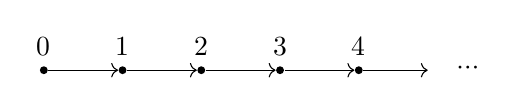
\begin{tikzpicture}
[n/.style={circle,fill=black,inner sep=0pt,minimum size=1mm}]
\node[n] (0) at (0,0) {};
\node[n] (1) at (1,0) {};
\node[n] (2) at (2,0) {};
\node[n] (3) at (3,0) {};
\node[n] (4) at (4,0) {};
\node (5) at (5,0) {};
\node[black,above] at (0.north) {$0$};
\node[black,above] at (1.north) {$1$};
\node[black,above] at (2.north) {$2$};
\node[black,above] at (3.north) {$3$};
\node[black,above] at (4.north) {$4$};
\node[black,right] at (5.east) {$\cdots$};
\draw[->] (0) -- (1);
\draw[->] (1) -- (2);
\draw[->] (2) -- (3);
\draw[->] (3) -- (4);\iffalse<<<<\fi
\draw[->] (4) -- (5);
\end{tikzpicture}
\end{center}
What is the ultrafilter extension of \(\fN\)? There are two kinds of
ultrafilter over an infinite set: the principal ultrafilter that are in
one-to-one correspondence with the points of the set, and the non-principal
ones which contain all co-finite sets and only infinite sets, cf Exercise
\ref{ex2.5.4}. The principal ultrafilters form an isomorphic copy of the frame
\(\fN\) inside \(\ue\fN\). For any pair \(u,u'\) of ultrafilters, if \(u'\)
is non-principal, then \(R^{ue}uu'\). To set this, let \(X\in u'\). As
\(X\) is infinite, for any \(n\in\N\) there is an \(m\) s.t. \(n<m\) and
\(m\in X\). This show that \(m_<(X)=\N\). But \(\N\) is an element of every
ultrafilter

The shows that the ultrafilter extension of \(\fN\) consists of a copy of
\(\fN\) followed by a uncountable cluster consisting of all the
non-principal ultrafilters
\end{examplle}

\begin{proposition}[]
\label{prop2.59}
Let \(\tau\) be a modal similarity type, and \(\fM\) a \(\tau\)-model. Then for any
formula \(\phi\) and any ultrafilter \(u\) over \(W\), \(V(\phi)\in u\) iff
\(\ue\fM,u\models\phi\). Hence for every state \(w\) of \(\fM\) we have
\(w\leftrightsquigarrow \pi_w\)
\end{proposition}

\begin{proof}
The second claim of the proposition is immediate from the first one by the
observation that \(w\Vdash\phi\) iff \(w\in V(\phi)\) iff \(V(\phi)\in\pi_w\)

Induction on \(\phi\). The basic case is immediate from the definition of
\(V^{ue}\). Suppose \(\phi\) is of the form \(\neg\psi\), then
\begin{align*}
V(\neg\psi)\in u&\quad\text{ iff }\quad
W\setminus V(\psi)\in u\\
&\quad\text{ iff }\quad V(\psi)\not\in u\\
&\quad\text{ iff }\quad \ue\fM,u\not\Vdash\psi\quad\text{IH}\\
&\quad\text{ iff }\quad \ue\fM,u\Vdash\neg\psi
\end{align*}

Now consider the case where \(\phi\) is of the form \(\diamond\psi\). Assume first
that \(\ue\fM,u\Vdash\diamond\psi\). Then there is an ultrafilter \(u'\)
s.t. \(R^{ue}uu'\) and \(\ue\fM,u'\Vdash\psi\). The induction hypothesis
implies that \(V(\psi)\in u'\), so by the definition of \(R^{ue}\),
\(m_R(V(\psi))\in u\). Now the result follows immediately from the observation
that \(m_R(V(\psi))=V(\diamond\psi)\)

Assume that \(V(\diamond\psi)\in u\). We have to find an ultrafilter \(u'\)
s.t. \(V(\psi)\in u'\) and \(R^{ue}uu'\). The latter constraint reduces to the
condition that \(m_R(X)\in u\) whenever \(X\in u'\), or equivalently (see
Exercise \ref{ex2.5.5})
\begin{equation*}
u_0':=\{Y\mid l_R(Y)\in u\}\subseteq u'
\end{equation*}
We will first show that \(u_0'\) is closed under intersection. Let \(Y,Z\in
    u_0'\). By definition, \(l_R(Y)\) and \(l_R(Z)\) are in \(u\). But then
\(l_R(Y\cap Z)\in u\) as \(l_R(Y\cap Z)=l_R(Y)\cap l_R(Z)\). This proves
that \(Y\cap Z\in u_0'\)

Next we make sure that for any \(Y\in u_0'\), \(Y\cap V(\psi)\neq\emptyset\).
Let \(Y\) be an arbitrary element of \(u_0'\), then by definition of
\(u_0'\), \(l_R(Y)\in u\). As \(u\) is closed under intersection and does
not contain the empty set, there must be an element \(x\in l_R(Y)\cap
    V(\diamond\psi)\). But then \(x\) must have a successor \(y\) in \(V(\psi)\).
Finally, \(x\in l_R(Y)\) implies \(y\in Y\)

From the fact that \(u_0'\) is closed under intersection, and the fact that
for any \(Y\in u_0'\), \(Y\cap V(\psi)\neq\emptyset\), it follows that the set
\(u_0'\cup\{V(\psi)\}\) has the finite intersection property. So the
Ultrafilter Theorem provides us with an ultrafilter \(u'\) s.t.
\(u_0'\cup\{V(\psi)\}\subseteq u'\). This ultrafilter \(u'\) has the desired
properties: it is clearly a successor of \(u\), and the fact the
\(\ue\fM,u'\Vdash\psi\) follows from \(V(\psi)\in u'\) and the induction hypothesis
\end{proof}

\begin{examplle}[]
Our new invariance result can be used to compare the relative expressive
power of modal languages. Consider the modal constant
\(\acwopencirclearrow\) whose truth definition in a model for the basic
modal language is
\begin{equation*}
\fM,w\Vdash\acwopencirclearrow \quad\text{ iff }\quad
\fM\models Rxx[v]\text{ for some $v$ in }\fM
\end{equation*}
Comparing the pictures of the frame \((\N,<)\) and its ultrafilter extension
given in Example \ref{example2.58} . The former is loop-free but the latter
contains uncountably many loops
\end{examplle}

\begin{proposition}[]
\label{prop2.61}
Let \(\tau\) be a modal similarity type, and let \(\fM\) be a \(\tau\)-model. Then
\(\ue\fM\) is \(m\)-saturated
\end{proposition}

\begin{proof}
Let \(\fM=(W,R,V)\) be a model. Consider an ultrafilter \(u\) over \(W\),
and a set \(\Sigma\) of modal formulas which is finitely satisfiable in the set of
successors of \(u\). We have to find an ultrafilter \(u'\) s.t.
\(R^{ue}uu'\) and \(\ue\fM,u'\Vdash\Sigma\). Define
\begin{equation*}
\Delta=\{V(\phi)\mid\phi\in\Sigma'\}\cup\{Y\mid l_R(Y)\in u\}
\end{equation*}
where \(\Sigma'\) is the set of (finite) conjunctions of formulas in \(\Sigma\). We
claim that the set \(\Delta\) has the finite intersection property. Since both
\(\{V(\phi)\mid\phi\in\Sigma'\}\) and \(\{Y\mid l_R(Y)\in u\}\) are closed
under taking intersections, it suffices to prove that for an arbitrary
\(\phi\in\Sigma'\) and an arbitrary set \(Y\subseteq W\) for which
\(l_R(Y)\in u\), we have \(V(\phi)\cap Y\neq\emptyset\). but if
\(\phi\in\Sigma'\), then by assumption, there is a successor \(u''\) of u
s.t. \(\ue\fM,u''\Vdash\phi\), or in other words, \(V(\phi)\in u''\). Then
\(l_R(Y)\in u\) implies \(Y\in u''\) by Exercise \ref{ex2.5.5} . Hence
\(V(\phi)\cap Y\) is an element of the ultrafilter \(u''\) and therefore cannot
be identical to the empty set.

It follows by the Ultrafilter Theorem that \(\Delta\) can be extended to an
ultrafilter \(u'\). Clearly \(u'\) is the required successor
\end{proof}

\begin{theorem}[]
Let \(\tau\) be a modal similarity type, and let \(\fM\) and \(\fM'\) be
\(\tau\)-models, and \(w,w'\) two states in \(\fM\) and \(\fM'\) respectively.
Then
\begin{equation*}
\fM,w\leftrightsquigarrow \fM',w' \quad\text{ iff }\quad
\ue\fM,\pi_w\leftrightarroweq\ue\fM',\pi_{w'}
\end{equation*}
\end{theorem}

\begin{proof}
From Propositions \ref{prop2.59}, \ref{prop2.61} and \ref{prop2.54}
\end{proof}


\begin{exercise}
\label{ex2.5.4}
Let \(W\) be an infinite set. Recall that \(X\subseteq W\) is \textbf{co-finite} if
\(W\setminus X\) is finite
\begin{enumerate}
\item Prove that the collection of co-finite subsets of \(W\) has the finite
intersection property
\item Show that there are ultrafilters over \(W\) that do not contain any
finite set
\item Prove that an ultrafilter is non-principal iff it contains only infinite
sets iff it contains all co-finite sets
\item Prove that any ultrafilter over \(W\) has uncountably many elements
\end{enumerate}
\end{exercise}



\begin{proof}
Suppose \(U=\{X\subseteq W\mid X\text{ is cofinite}\}\)
\begin{enumerate}
\item For any \(A,B\in U\), if \(A\cap B=\empty\), \(A\subset\bbar{B}\). But
\(A\) is infinite and \(\bbar{B}\) is finite, this can't happen. Hence
\(A\cap B\neq\emptyset\)
\item \(U\) can be extended to a ultrafilter \(\calu\). If \(A\) is finite, then
\(\bbar{A}\in U\subseteq\calu\). Hence \(\calu\) does not contain any
finite set.
\item \(1\to 2\).If an ultrafilter contains a finite set. Then its a principal ultrafilter
generated on the intersection of all finite sets.

\(2\to3\) and \(3\to1\) are obvious.
\item Half of the \(\calp(W)\) belongs to the ultrafilter and \(\calp(W)\) is uncountable
\end{enumerate}
\end{proof}

\begin{exercise}
\label{ex2.5.5}
Given a model \(\fM=(W,R,V)\) and two ultrafilters \(u\) and \(v\) over
\(W\), show that \(R^{ue}uv\)iff \(\{Y\mid l_R(Y)\in u\}\subseteq v\)
\end{exercise}

\begin{proof}
\begin{align*}
R^{ue}uv&\Leftrightarrow
X\in v\to m_R(X)\in u\\
&\Leftrightarrow \neg m_R(X)\in u\to \neg X\in v \\
&\Leftrightarrow W-m_R(X)\in u\to W-X\in v\\
&\Leftrightarrow l_R(W-X)\in u\to W-X\in v\\
&(\text{Since }m_R(X)=W-l_R(W-X))\\
&\Leftrightarrow\{Y\mid l_R(Y)\in u\}\subseteq v
\end{align*}
\end{proof}
\subsection{Characterization and Definability}
\label{sec:org31eb5b0}
\subsubsection{The van Benthem Characterization Theorem}
\label{sec:orgffdc89f}
Let \(\Gamma(x)\) be a set of first-order formulas in which a single individual
variable may occur free - such a set of formulas is called a \textbf{type}. A
first-order model \(\fM\) \textbf{realizes} \(\Gamma(x)\) if there is an element \(w\) in
\(\fM\) s.t. for all \(\gamma\in\Gamma,\fM\models\gamma[w]\)

Let \(\fM\) be a model for a given first-order language \(\call^1\) with
domain \(W\). For a subset \(A\subset W\), \(\call^1[A]\) is the language
obtained by extending \(\call^1\) with new constant \(\underline{a}\) for
all elements \(a\in A\). \(\fM_A\) is the expansion of \(\fM\) to a
structure for \(\call^1[A]\) in which each \(\underline{a}\) is interpreted
as \(a\)

Assume that \(A\) is of size at most \(\alpha\). Assume that \(\alpha=3\) and
\(A=\{\alpha_1,\alpha_2\}\). Let \(\Gamma(\und{a}_1,\und{a}_2,x)\) be a type of
the language \(\call^1[A]\); \(\Gamma(\und{a}_1,\und{a}_2,x)\) is consistent with
the first-order theory of \(\fM_A\) iff \(\Gamma(\und{a}_1,\und{a}_2,x)\) is
finitely realizable in \(\fM_A\). So for this particular set
\(\Gamma(\und{a}_1,\und{a}_2,x)\), 3-saturation of \(\fM\) means that if
\(\Gamma(\und{a}_1,\und{a}_2,x)\) is finitely realizable in \(\fM_A\), then
\(\Gamma(\und{a}_1,\und{a}_2,x)\) is realizable in \(\fM_A\)

Or consider a formula \(\gamma(\und{a}_1,\und{a}_2,x)\) and let \(\gamma(x_1,x_2,x)\)
be the formula with the fresh variables \(x_1\) and \(x_2\) replacing each
occurrence in \(\gamma\) of \(\und{a}_1\) and \(\und{a}_2\) respectively. Then we
have the following equivalence

\begin{center}
\(\fM_A\) realizes \(\{\gamma(\und{a}_1,\und{a}_2,x)\}\) iff there is a \(b\)
s.t. \(\fM\models\gamma(x_1,x_2,x)[a_1,a_2,b]\)
\end{center}

So a model is \(\alpha\)-saturated iff the following holds for every
\(n<\alpha\) and every set \(\Gamma\) of formulas of the form \(\gamma(x_1,\dots,x_n,x)\)

\begin{center}
\textbf{If} \((a_1,\dots,a_n)\) is an \(n\)-tuple s.t. for every finite
\(\Delta\subseteq\Gamma\) there is a \(b_{\Delta}\) s.t.
\(\fM\models\gamma(x_1,\dots,x_n,x)[a_1,\dots,a_n,b_\Delta]\) for every
\(\gamma\in\Delta\)


\textbf{then} we have that there is a \(b\) s.t.
 \(\fM\models\gamma(x_1,\dots,x_n,x)[a_1,\dots,a_n,b]\) for every \(\gamma\in\Gamma\)
\end{center}


\begin{definition}[]
Let \(\alpha\) be a natural number, or \(\omega\). A model \(\fM\) is \textbf{\(\alpha\)-saturated}
if for  every subset \(A\subseteq W\) of size less than \(\alpha\), the expansion
\(\fM_A\) realizes every set \(\Gamma(x)\) of \(\call^1[A]\)-formulas (with only
\(x\) occurring free) that is \emph{consistent} (a proof-theoretic notion, only
finite deductions, hence this definition is consistent the definition above)
with the first-order theory of
\(\fM_A\). An \(\omega\)-saturated model is usually called \textbf{countably saturated}
\end{definition}

\begin{examplle}[]
\begin{enumerate}
\item Every finite model is countably saturated. For if \(\fM\) is finite, and
\(\Gamma(x)\) is a set of first-order formulas consistent with the first-order
theory of \(\fM\), there exists a model \(\fN\) that is elementarily
equivalent to \(\fM\) and that realizes \(\Gamma(x)\). But as \(\fM\) and
\(\fN\) are finite, elementary equivalence implies isomorphism
(\href{https://math.stackexchange.com/questions/1518629/a-simple-proof-that-elementary-equivalence-and-isomorphism-coincide-for-finite-s}{proof})
, and hence
\(\Gamma(x)\) is realized in \(\fM\)
\item The ordering of the rational numbers \((\Q,<)\) is countably saturated as
well. The relevant first-order language \(\call^1\) has \(<\) and \(=\).
Take a subset \(A\) of \(\Q\) and let \(\Gamma(x)\) be a set of formulas in the
resulting expansion \(\call^1[A]\) of the first-order language that is
consistent with the theory of \((\Q,<,a)_{a\in A}\). Then there exists a
model \(\fN\) of the theory of \((\Q,<,a)_{a\in A}\) that realizes
\(\Gamma(x)\). \(\star\).
Now take a countable elementary submodel \(\fN'\) of \(\fN\) that
contains at least one object realizing \(\Gamma(x)\). Then \(\fN'\) is a
countable dense linear ordering without endpoints, and hence the ordering
of \(\fN'\) is isomorphic to \((\Q,<)\).
\end{enumerate}
\end{examplle}

\begin{theorem}[]
\label{thm2.65}
Let \(\tau\) be a modal similarity type. Any countably saturated \(\tau\)-model is
\(m\)-saturated. It follows that the class of countably saturated
\(\tau\)-models has the Hennessy-Milner property
\end{theorem}

\begin{proof}
Assume that \(\fM=(W,R,V)\) viewed as a first-order model, is countably
saturated. Let \(a\) be a state in \(W\), and consider a set \(\Sigma\) of modal
formulas which is finite satisfiable in the successor set of \(a\). Define
\(\Sigma'\) to be the set
\begin{equation*}
\Sigma'=\{R\und{a}x\}\cup ST_x(\Sigma)
\end{equation*}
where \(ST_x(\Sigma)=\{ST_x(\phi)\mid\phi\in\Sigma\}\). \(\Sigma'\) is consistent
with the first-order theory of \(\fM_a\): \(\fM_a\) realizes every finite
subset of \(\Sigma'\), namely in some successor of \(a\). So by the
countable saturation of \(\fM\), \(\Sigma'\) is realized in some state
\(b\). By \(\fM_A\models R\und{a}x[b]\) it follows that \(b\) is a successor
of \(a\). Then, by Proposition \ref{prop2.47} and the fact that \(\fM_a\models
    ST_x(\phi)[b]\) for all \(\phi\in\Sigma\), it follows that
\(\fM,b\Vdash\Sigma\). Thus \(\Sigma\) is satisfiable in a successor of \(a\)
\end{proof}

\begin{lemma}[Detour Lemma]
Let \(\tau\) be a modal similarity type, and let \(\fM\) and \(\fN\) be two models,
and \(w\) and \(v\) states in \(\fM\) and \(\fN\), respectively. Then the
following are equivalent:
\begin{enumerate}
\item For all modal formulas \(\phi\): \(\fM,w\Vdash\phi\) iff \(\fN,v\Vdash\phi\)
\item There exists a bisimulation \(Z:\ue\fM,\pi_w\leftrightarroweq\ue\fN,\pi_v\)
\item There exist countably saturated models \(\fM^*,w^*,\fN^*,v^*\) and elementary
embeddings \(f:\fM\preceq\fM^*\) and \(g:\fN\preceq\fN^*\) s.t.
\begin{enumerate}
\item \(f(w)=w^*\) and \(g(v)=v^*\)
\item \(\fM^*,w^*\leftrightarroweq\fN^*,v^*\)
\end{enumerate}
\end{enumerate}
\end{lemma}

\begin{definition}[]
A first-order formula \(\alpha(x)\) in \(\call^1_\tau\) is \textbf{invariant for
bisimulations} if for all models \(\fM\) and \(\fN\), and all states \(w\) in
\(\fM\), \(v\) in \(\fN\), and all bisimulations \(Z\) between \(\fM\) and
\(\fN\) s.t. \(wZv\), we have \(\fM\models\alpha(x)[w]\) iff \(\fN\models\alpha(x)[v]\)
\end{definition}

\begin{theorem}[van Benthem Characterization Theorem]
Let \(\alpha(x)\) be a first-order formula in \(\call_\tau^1\). Then \(\alpha(x)\) is
invariant for bisimulations iff it is equivalent to the standard translation
of a modal \(\tau\)-formula
\end{theorem}

\begin{proof}
Assume \(\alpha(x)\) is invariant for bisimulations and consider the set of modal
consequences of \(\alpha\):
\begin{equation*}
MOC(\alpha)=\{ST_x(\phi)\mid\phi\text{ is a modal formula, and }\alpha(x)\models ST_x(\phi)\}
\end{equation*}
Our first claim is that if \(MOC(\alpha)\models\alpha(x)\), then \(\alpha\) is
equivalent to the translation of a modal formula.  Assume
\(MOC(\alpha)\models\alpha(x)\), then by the Compactness Theorem for first-order
logic, for some finite subset \(X\subseteq MOC(\alpha)\), we have
\(X\models\alpha(x)\). So \(\models\bigwedge X\to\alpha(x)\). Trivially
\(\models\alpha(x)\to\bigwedge X\), thus
\(\models\alpha(x)\leftrightarrow\bigwedge X\). And as every \(\beta\in X\)
is the translation of a modal formula, so is \(\bigwedge X\)

So it suffices to show that \(MOC(\alpha)\models\alpha(x)\). Assume
\(\fM\models
    MOC(\alpha)[w]\); we need to show that \(\fM\models\alpha(x)[w]\). Let
\begin{equation*}
T(x)=\{ST_x(\phi)\mid\fM\models ST_x(\phi)[w]\}
\end{equation*}
We claim that \(T(x)\cup\{\alpha(x)\}\) is consistent. Assume that
\(T(x)\cup\{\alpha(x)\}\) is inconsistent. Then by compactness, for some finite
subset \(T_0(x)\subset T(x)\) we have \(\models\alpha(x)\to\neg\bigwedge
    T_x(x)\). Hence \(\neg\bigwedge T_0(x)\in MOC(\alpha)\). But this implies
\(\fM\models\neg\bigwedge T_0(x)[w]\), a contradiction

Let \(\fN,v\) be s.t. \(\fN\models T(x)\cup\{\alpha(x)\}[v]\). Observe that \(w\)
and \(v\) are modally equivalent: \(\fM,w\Vdash\phi\) implies \(ST_x(\phi)\in
    T(x)\), which implies \(\fN,v\Vdash\phi\); and likewise, if
\(\fM,w\not\Vdash\phi\) then \(\fM,w\Vdash\neg\phi\) and
\(\fN,v\Vdash\neg\phi\).


We can use the Detour Lemma and make a detour through a Hennessy-Milner
class where modal equivalence and bisimilarity do coincide.
\begin{center}
    \begin{tikzcd}
\fM,w\arrow[d,dash,"\preceq"]&\fN,v\arrow[d,dash,"\preceq"]\\
\fM^*,w^*\arrow[r,"\leftrightarroweq",dash]&\fN^*,v^*
\end{tikzcd}
\end{center}
\(\fN\models\alpha(x)[v]\) implies \(\fN^*\models\alpha(x)[v^*]\). As
\(\alpha(x)\) is invariant for bisimulations, we get
\(\fM^*\models\alpha(x)[w^*]\). By invariance under elementary embeddings,
we have \(\fM\models\alpha(x)[w]\)
\end{proof}


\subsubsection{Ultraproducts}
\label{sec:org6ee03d2}

Suppose \(I\neq\emptyset\), \(U\) is an ultrafilter over \(I\).
\begin{definition}[Ultraproducts of Sets]
Let \(f_U\) be the equivalence class of \(f\) modulo \(\sim_U\), that is:
\(f_U=\{g\in C\mid g\sim_U f\}\). The \textbf{ultraproduct of \(W_i\) modulo} \(U\),
denoted as \(\prod_UW_i\) is the set of all equivalence classes of
\(\sim_U\). So
\begin{equation*}
\prod_UW_i=\{f_U\mid f\in\prod_{i\in I}W_i\}
\end{equation*}
In case \(W_i=W\), the ultraproduct is called the \textbf{ultrapower of \(W\) modulo}
\(U\), and written \(\prod_UW\)
\end{definition}

\begin{definition}[Ultraproduct of Models]
Fix a modal similarity type \(\tau\), and let \(\fM_i(i\in I)\) be \(\tau\)-models.
The \textbf{ultraproduct} \(\prod_U\fM_i\) of \(\fM_i\) modulo \(U\) is the model
described as follows
\begin{enumerate}
\item The universe \(W_U\) of \(\prod_U\fM_i\) is the set \(\prod_UW_i\)
\item Let \(V_i\) be the valuation of \(\fM_i\). Then the valuation \(V_U\) of
\(\prod_U\fM_i\) is defined by
\begin{equation*}
f_U\in V_U(p) \quad\text{ iff }\quad
\{i\in I\mid f(i)\in V_i(p)\}\in U
\end{equation*}
\item Let \(\triangle\) be a modal operator in \(\tau\), and \(R_{\triangle i}\) its
associated relation in the model \(\fM_i\). The relation \(R_{\triangle
       U}\) in \(\prod_U\fM_i\) is given by
\begin{equation*}
R_{\triangle U}f_U^1\dots f_U^{n+1} \quad\text{ iff }\quad
\{i\in I\mid R_{\triangle i}f^1(i)\dots f^{n+1}(i)\}\in U
\end{equation*}
\end{enumerate}


In particular,
\begin{equation*}
R_{\diamond U}f_Ug_U \quad\text{ iff }\quad
\{i\in I\mid R_{\diamond i}f(i)g(i)\}\in U
\end{equation*}
\end{definition}

\begin{proposition}[]
Let \(\prod_U\fM\) be an ultrapower of \(\fM\). Then for al modal formulas \(\phi\)
we have \(\fM,w\Vdash\phi\) iff \(\prod_U\fM,(f_w)_U\Vdash\phi\), where
\(f_w\) is the constant function s.t. \(f_w(i)=w\) for all \(i\in I\)
\end{proposition}

\begin{proof}
\begin{enumerate}
\item \(\phi=p\)
\begin{align*}
\fM,w\Vdash\phi&\Leftrightarrow w\in V(\phi)\\&\Leftrightarrow
\{i\in I\mid f_w(i)\in V(p)\}=I\in U\\&\Leftrightarrow
\prod_U\fM,(f_w)_U\Vdash\phi
\end{align*}
\item \(\phi=\diamond\psi\)
\begin{equation*}
Rwv\Leftrightarrow\{i\in I\mid R_{\diamond i}f_w(i)f_v(i)\}=I\in U\Leftrightarrow
R_{\diamond U}f_wg_v
\end{equation*}
\end{enumerate}
\end{proof}

An ultrafilter is \textbf{countably incomplete} if it is not closed under countably intersections

\begin{examplle}[]
Consider the set of natural numbers \(\N\). Let \(U\) be an ultrafilter over
\(\N\) that does not contain any singletons \(\{u\}\). Then for all \(n\),
\((\N\setminus\{n\})\in U\). But
\begin{equation*}
\emptyset=\bigcap_{n\in\N}(\N\setminus\{n\})\not\in U
\end{equation*}
So \(U\) is countably incomplete
\end{examplle}

\begin{lemma}[]
\label{lemma2.73}
Let \(\call\) be a countable first-order language, \(U\) a countably
incomplete ultrafilter over a non-empty set \(I\), and \(\fM\) an
\(\call\)-model. The ultrapower \(\prod_U\fM\) is countably saturated
\end{lemma}

\begin{theorem}[]
\label{thm2.74}
Let \(\tau\) be a modal similarity type, and let \(\fM\) and \(\fN\) be
\(\tau\)-models, and \(w\) and \(v\) states in \(\fM\) and \(\fN\)
respectively. Then the following are equivalent
\begin{enumerate}
\item For all modal formulas \(\phi\): \(\fM,w\Vdash\phi\) iff \(\fN,v\Vdash\phi\)
\item There exists ultrapowers \(\prod_U\fM\) and \(\prod_U\fN\) as well as a
bisimulation \(Z:\prod_U\fM,(f_w)_U\leftrightarroweq\prod_U\fN,(f_v)_U\)
linking \((f_w)_U\) and \((f_v)_U\), where \(f_w(f_v)\) is the constant
function mapping every index to \(w(v)\)
\end{enumerate}
\end{theorem}

\begin{proof}
\(2\to1\). \(\fM,w\Vdash\phi\) iff \(\prod_U\fM,(f_w)_U\Vdash\phi\) iff
\(\prod_U\fN,(f_v)_U\Vdash\phi\) iff \(\fN,v\Vdash\phi\)

\(1\to2\). Take \(\N\) as our index set, and let \(U\) be a countably
incomplete ultrafilter over \(\N\). By Lemma \ref{lemma2.73} the ultrapowers
\(\prod_U\fM\) and \(\prod_U\fN\) are countably saturated. Now \((f_w)_U\)
and \((f_v)_U\) are modally equivalence. Next apply Theorem \ref{thm2.65}: as
\((f_w)_U\) and \((f_v)_U\) are modally equivalent and \(\prod_U\fM\) and
\(\prod_U\fN\) are countably saturated, there exists a bisimulation
\end{proof}

\subsubsection{Definability}
\label{sec:orgb4da68e}
Given a modal similarity type \(\tau\), a pointed model is a pair \((\fM,w)\) where
\(\fM\) is a \(\tau\)-model and \(w\) is a state of \(\fM\). A class of
pointed models \(\sfK\) is said to be \textbf{closed under bisimulations} if
\((\fM,w)\in\sfK\) and \(\fM,w\leftrightarroweq\fN,v\) implies
\((\fN,v)\in\sfK\). \(\sfK\) is \textbf{closed under ultraproducts} if any
ultraproducts \(\prod_U(\fM_i,w_i)\) of a family of pointed models
\((\fM_i,w_i)\) in \(K\) belongs to \(\sfK\). If \(\sfK\) is a class of
pointed \(\tau\)-models, \(\bbar{\sfK}\) denotes the complement of \(\sfK\)
within the class of all pointed \(\tau\)-models. \(\sfK\) is
\textbf{definable by a set of modal formulas} if there is a set of modal formulas \(\Gamma\)
s.t. for any pointed model \((\fM,w)\) we have \((\fM,w)\) in \(\sfK\) iff
for all \(\gamma\in\Gamma,\fM,w\Vdash\gamma\). \(\sfK\) is definable by a
single modal formula iff it is definable by a singleton set

By Theorem \ref{thm2.20} definable classes of pointed models must be closed
under bisimulations, and by Proposition \ref{prop2.47} and Corollary
\ref{corA.20} they must be closed under ultraproducts as well.

\begin{theorem}[]
\label{thm2.75}
Let \(\tau\) be a modal similarity type, and \(\sfK\) a class of pointed
\(\tau\)-models. Then the following are equivalent:
\begin{enumerate}
\item \(\sfK\) is definable by a set of modal formulas
\item \(\sfK\) is closed under bisimulations and ultraproducts, and
\(\bbar{K}\) is closed under ultrapowers
\end{enumerate}
\end{theorem}

\begin{proof}
Assume \(\sfK\) and \(\bbar{\sfK}\) satisfy the stated closure conditions.
Observe that \(\bbar{\sfK}\) is closed under bisimulations as \(\sfK\) is.
Define
\begin{equation*}
T=\{\phi\mid\forall(\fM,w)\in\sfK:\fM,w\Vdash\phi\}
\end{equation*}
We will show that \(T\) defines the class of \(\sfK\).

Assume \(\fM,w\Vdash T\). Define \(\Sigma=\{\phi\mid\fM,w\Vdash\phi\}\). It is
obvious that \(\Sigma\) is finitely satisfiable in \(\sfK\); for suppose that the set
\(\{\sigma_1,\dots,\sigma_n\}\subseteq\Sigma\) is not satisfiable in
\(\sfK\). Then the formula \(\neg(\sigma_1\wedge\dots\wedge\sigma_n)\) would
be true on all pointed models in \(\sfK\), so it would belong to \(T\), yet
be false in \(\fM,w\). But then the following claim shows that \(\Sigma\) is
satisfiable in the ultraproduct of pointed models

\textbf{Claim 1} . Let \(\Sigma\) be a set of modal formulas, and \(\sfK\) a class of pointed
 models in which \(\Sigma\) is finitely satisfiable. Then \(\Sigma\) is satisfiable in some
 ultraproduct of models in \(\sfK\)

\emph{Proof of Claim.} Define in index set \(I\) as the collection of all finite
subsets of \(\Sigma\)
\begin{equation*}
I=\{\Sigma_0\subset\Sigma\mid \Sigma_0\text{ is finite}\}
\end{equation*}
By assumption, for each \(i\in I\) there is a pointed model \((\fN_i,v_i)\)
in \(\sfK\) s.t. \(\fN_i,v_i\Vdash i\). We now construct an ultrafilter
\(U\) over \(I\) s.t. the ultraprodcut \(\prod_U\fN_i\) has a state \(f_U\)
with \(\prod_U\fN_i,f_U\Vdash\Sigma\)

For each \(\sigma\in\Sigma\), let \(\widehat{\sigma}\) be the set of all \(i\in
     I\) s.t. \(\sigma\in i\). Then the set
\(E=\{\widehat{\sigma}\mid\sigma\in\Sigma\}\) has the finite intersection
property because
\begin{equation*}
\{\sigma_1,\dots,\sigma_n\}\in\widehat{\sigma}_1\cap\dots\cap\widehat{\sigma}_n
\end{equation*}
So \(E\) can be extended to an ultrafilter \(U\) over \(I\). This defines
\(\prod_U\fN_i\); for the definition of \(f_U\), let \(W_i\) denote the
universe of the model \(\fN_i\) and consider the function \(f\in\prod_{i\in
     I}W_i\) s.t. \(f(i)=v_i\).
It is left to prove that
\begin{equation*}
\prod_U\fN_i,f_U\Vdash\Sigma
\end{equation*}
Observe that for \(i\in\widehat{\sigma}\) we have \(\sigma\in i\) and so
\(\fN_i,v_i\Vdash\sigma\). Therefore for each \(\sigma\in\Sigma\)
\begin{equation*}
\{i\in I\mid\fN_i,v_i\Vdash\sigma\}\supseteq\widehat{\sigma} \quad\text{ and }\quad
\widehat{\sigma}\in U
\end{equation*}
since \(\sigma\in i\) implies \(\fN_i,v_i\Vdash\sigma\). It follows that
\(\{i\in I\mid\fN_i,v_i\Vdash\sigma\}\in U\), so by Theorem \ref{thmA.19}
\(\prod_U\fN_i,f_U\Vdash\sigma\). Hence \(\prod_U\fN_i,f_U\Vdash\Sigma\)

It follows from Claim 1 and the closure of \(\sfK\) under taking
ultraproducts that \(\Sigma\) is satisfiable in some pointed model
\((\fN,v)\in\sfK\). But \(\fN,v\Vdash\Sigma\) implies that \(v\) and the
state \(w\)  from our \uline{original pointed model \((\fM,w)\) are modally
equivalent}. So by Theorem \ref{thm2.74} there exists an ultrafilter \(U'\)
s.t.
\begin{equation*}
\prod_{U'}(\fN,v),(f_v)_U\leftrightarroweq
\prod_{U'}(\fM,w),(f_w)_U
\end{equation*}
By closure under ultraproducts, the pointed model
\((\prod_{U'}(\fN,v),(f_v)_U)\) belongs to \(\sfK\). Hence by closure under
bisimulations, \((\prod_{U'}(\fM,w),(f_w)_U)\) is in \(\sfK\). By closure
of \(\bbar{K}\) under ultrapowers, \((\fM,w)\in\sfK\)
\end{proof}

\begin{theorem}[]
\label{thm2.76}
Let \(\tau\) be a modal similarity type, and \(\sfK\) a class of pointed
\(\tau\)-models. Then the following are equivalent
\begin{enumerate}
\item \(\sfK\) is definable by means of a single modal formula
\item Both \(\sfK\) and \(\bbar{\sfK}\) are closed under bisimulations and ultraproducts
\end{enumerate}
\end{theorem}

\begin{proof}
Assume \(\sfK,\bbar{\sfK}\) satisfy the stated conditions. Then both are
closed under ultraproducts, hence by Theorem \ref{thm2.75} there are set of
modal formulas \(T_1,T_2\) defining \(\sfK\) and \(\bbar{\sfK}\)
respectively. Observe their union is inconsistent in the sense that there is
no pointed model \((\fM,w)\) s.t. \((\fM,w)\Vdash T_1\cup T_2\). So by
compactness there exists \(\phi_1,\dots,\phi_n\in T_1\) and
\(\psi_1,\dots,\psi_m\in T_2\) s.t. for all pointed models \((\fM,w)\)
\begin{equation*}
\fM,w\Vdash\phi_1\wedge\dots\wedge\phi_n\to\neg\psi\vee\dots\vee\neg\psi_m
\end{equation*}
By definition, for any \((\fM,w)\in\sfK\) we have
\(\fM,w\Vdash\phi_1\wedge\dots\wedge\phi_n\). Conversely, if
\(\fM,w\Vdash\phi_1\wedge\dots\wedge\phi_n\), then
\(\fM,w\Vdash\neg\psi_1\vee\dots\vee\neg\psi_m\). Hence \(\fM,w\not\Vdash
    T_2\). Therefore \((\fM,w)\not\in\bbar{\sfK}\), whence \((\fM,w)\in\sfK\)
\end{proof}




\section{Frames}
\label{sec:orgead8038}

\subsection{Frame Definability}
\label{sec:org7dbcb18}
\begin{definition}[Validity]
Let \(\tau\) be a modal similarity type. A formula \(\phi\) (of this similarity type) is
\textbf{valid at a state \(w\) in a frame \(\fF\)} (notation: \(\fF,w\Vdash\phi\)) if
\(\phi\) is true at \(w\) in every model \((\fF,V)\) based on \(\fF\); \(\phi\) is
\textbf{valid on a frame \(\fF\)} (notation: \(\fF\Vdash\phi\)) if it is valid at
every state in \(\fF\). A formula \(\phi\) is \textbf{valid on a class of frames \(\sfK\)}
(notation: \(\sfK\Vdash\phi\)) if it is valid on every frame \(\fF\) in
\(\sfK\). We denote the class of frames where \(\phi\) is valid by \(\sfFr_\phi\)

A set \(\Gamma\) of modal formulas (of type \(\tau\)) is \textbf{valid on a frame \(\fF\)} if every
formula in \(\Gamma\) is valid on \(\sfF\); and \(\Gamma\) is \textbf{valid on a class \(\sfK\) of
frames} if \(\Gamma\) is valid on every member of \(\sfK\). We denote the class of
frames where \(\Gamma\) is valid by \(\sfFr_\Gamma\)
\end{definition}

\begin{definition}[Definability]
Let \(\tau\) be a modal similarity type, \(\phi\) a modal formula of this type, and
\(\sfK\) a class of \(\tau\)-frames. We say that \(\phi\) \textbf{defines} (or \textbf{characterizes})
\(\sfK\) if for all frames \(\fF\), \(\fF\) is in \(\sfK\) iff
\(\fF\Vdash\phi\). Similarly, if \(\Gamma\) is a set of modal formulas of this type,
we say that \(\Gamma\) \textbf{defines} \(\fF\) is in \(\sfK\) iff \(\fF\Vdash\Gamma\)

A class of frames is \textbf{(modally) definable} if there is some set of modal
formulas that defines it
\end{definition}

\begin{definition}[Relative Definability]
Let \(\tau\) be a modal similarity type, \(\phi\) a modal formula of this type, and
\(\sfC\) a class of \(\tau\)-frames. We say that \(\phi\) \textbf{defines} (or \textbf{characterizes})
a class \(\sfK\) of frames \textbf{within} \(\sfC\) (or \textbf{relative to} \(\sfC\)) if for
all frames \(\fF\) in \(\sfC\) we have that \(\fF\) is in \(\sfK\) iff
\(\fF\Vdash\phi\)

Similarly, if \(\Gamma\) is a set of modal formulas of this type, we say that \(\Gamma\)
\textbf{defines} a class \(\sfK\) of frames \textbf{within} \(\sfC\) if for all frames \(\fF\)
in \(\sfC\) we  have that \(\fF\) is in \(\sfK\) iff \(\fF\Vdash\Gamma\)
\end{definition}

\begin{definition}[Frame Languages]
For any modal similarity type \(\tau\), the \textbf{first-order frame language} of \(\tau\) is the
first-order language that has the identity symbol = together with an
\((n+1)\)-ary relation symbol \(R_{\triangle}\) for each \(n\)-ary modal
operator \(\triangle\) in \(\tau\). We denote this language by \(\call_\tau^1\). We
often call it the \textbf{first-order correspondence language} (for \(\tau\))

Let \(\Phi\) be any set of proposition letters. The \textbf{monadic second-order frame
language} of \(\tau\) over \(\Phi\) is the monadic second-order language obtained by
augmenting \(\call_\tau^1\) with a \(\Phi\)-indexed collection of monadic
predicate variables. (That is, this language has all the resources of
\(\call_\tau^1\), and in addition is capable of quantifying over subsets of
frames). We denote this language by \(\call_\tau^2(\Phi)\). We often simply call it the
\textbf{second-order frame language} or the \textbf{second-order correspondence language} (for \(\tau\))
\end{definition}

\begin{definition}[Frame Correspondence]
If a class of frames (property) can be defined by a modal formula \(\phi\) and by a
formula \(\alpha\) from one of these frame languages, then we say that \(\phi\) and \(\alpha\) are
each others (global) frame \textbf{correspondents}
\end{definition}

For example the basic modal formula \(p\to\Diamond p\) and the first-order
sentence \(\forall xRxx\) are correspondents

\begin{examplle}[]
Read \(\Diamond\phi\) as 'it is \textbf{possibly} the case that \(\phi\) ' and \(\Box\phi\) as
'\textbf{necessarily} \(\phi\)  '.
\begin{itemize}
\item [(T)] \(p\to\Box p\)
\item [(4)] \(\Diamond\Diamond p\to\Diamond p\)
\item [(5)] \(\Diamond p\to\Box\Diamond p\)
\end{itemize}

Our first claim is that for any frame \(\fF=(W,R)\), the axiom T corresponds
to \textbf{reflexivity} of the relation \(R\):
\begin{equation*}
\fF\Vdash \text{T}\quad\text{ iff }\quad
\fF\Vdash\forall x\;Rxx
\end{equation*}
Suppose that \(R\) is \textbf{not} reflexive. There exists a state \(w\) which is not
accessible from itself. Now the valuation \(V\) has to satisfy two conditions
\begin{enumerate}
\item \(w\in V(p)\)
\item \(\{x\in W\mid Rwx\}\cap V(p)=\emptyset\)
\end{enumerate}


Consider the \textbf{minimal} valuation \(V\) satisfying condition (1), that is, take
\begin{equation*}
V(p)=\{w\}
\end{equation*}
Now let \(v\) be an \(R\)-successor of \(w\). As \(Rww\) does not hold in
\(\fF\), \(v\) must be distinct from \(w\), so \(v\not\Vdash p\). As \(v\)
was arbitrary, \(w\not\Vdash p\)

Likewise, one can prove that for any frame \(\fF=(W,R)\)
\begin{alignat*}{3}
&\fF\Vdash4&&\quad\text{ iff }\quad&&R\text{ is transitive}\\
&\fF\Vdash5\quad&&\quad\text{ iff }\quad&&
R \text{ is euclidean}
\end{alignat*}
where a relation is \textbf{euclidean} if it satisfies \(\forall xyz((Rxy\wedge
   Rxz)\to Ryz)\).

Assume \(\fF\) is a non-euclidean frame; then there must be states \(u,v,w\)
s.t. \(Ruv,Ruw\) but not \(Rvw\):
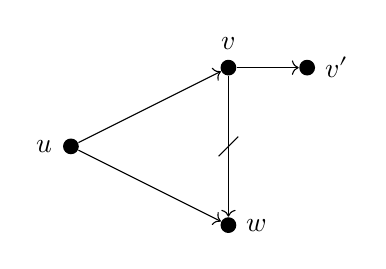
\begin{tikzpicture}
[n/.style={circle,fill=black,inner sep=0pt,minimum size=2mm}]
\node[n] (u) at (0,0) {};
\node[n] (v) at (2,1) {};
\node[n] (w) at (2,-1) {};
\node[n] (v') at (3,1) {};
\node[left] at (u.west) {$u$};
\node[right] at (v'.east) {$v'$};
\node[above] at (v.north) {$v$};
\node[right] at (w.east) {$w$};
\draw[->] (u) --(v);
\draw[->](u) --  (w);
\draw[->] (v) -- (v');
\draw[->] (v)--node[strike out,draw,-]{} (w);
\end{tikzpicture}
We will try to falsify 5 in \(u\); for this purpose we have to find a
valuation \(V\) s.t. \((\fF,V),u\Vdash\Diamond p\) and
\((\fF,V),u\not\Vdash\Box\Diamond p\). In other words, we have to make \(p\)
\textbf{true} at some \(R\)-successor \(x\) of \(u\), and \textbf{false} at all
\(R\)-successors of some \(R\)-successor \(y\) of \(u\). The constaints on
\(V\) are
\begin{enumerate}
\item \(w\in V(p)\)
\item \(\{z\mid Rvz\}\cap V(p)=\emptyset\)
\end{enumerate}


Let's take a \textbf{maximal} \(V\) satisfying condition (2), that is, define
\begin{equation*}
V(p)=\{z\in W\mid\text{ it is not the case that }Rvz\}
\end{equation*}
Now \(v\not\Vdash\Diamond p\), so \(u\not\Vdash\Box\Diamond p\). On the other
hand, we have \(w\Vdash p\), so \(u\Vdash\Diamond p\)
\end{examplle}

\begin{examplle}[]
Suppose that we are working with the basic temporal language and that we are
interested in \textbf{dense} bidirectional frames. This property can be defined using
a first-order sentence (namely \(\forall xy(x<y\to\exists z(x<z\wedge
   z<y))\)) but can the basic temporal language define it too?

The following simple formula suffices: \(Fp\to FFp\). Let \(\fT=(T,<)\) be a
frame s.t. \(\fT\Vdash Fp\to FFp\). Suppose that a point \(t\in T\) has a
<-successor \(t'\). Consider the following \textbf{minimal} valuation \(V_m\)
guaranteeing that \((\fT,V_m),t\Vdash Fp\)
\begin{equation*}
V_m(p)=\{t'\}
\end{equation*}
Hence \(t\Vdash FFp\). This means there is a point \(s\) s.t. \(t<s\) and
\(s\Vdash Fp\). But as \(t'\) is the \textbf{only} states where \(p\) holds, this
implies that \(s<t'\)
\end{examplle}

\begin{examplle}[]
Suppose we are working with a similarity type with three binary operators
\(\triangle_1,\triangle_2, \triangle_3\), and that we are interested in the
class of frames in which the three ternary accessibility relations (denoted
by \(R_1,R_2,R_3\) respectively, if \(R_1stu\) and \(s\Vdash p,t\Vdash
   q,s\Vdash r\), then \(s\Vdash q\triangle_1 r\)).

We want
\begin{equation*}
 R_1stu \quad\text{ iff }\quad R_2tus \quad\text{ iff }\quad
 R_3ust
\end{equation*}
to hold for all \(s,t,u\) in such frames. Can we define this class of frames?

We can. We will show that for all frames \(\calf=(W,R_1,R_2,R_3)\) we have
\begin{equation*}
 \calf\Vdash p\wedge(q\triangle_1 r)\to(q\wedge r\triangle_2 p)
 \triangle_1 r
 \quad\text{ iff }\quad \calf\Vdash\forall xyz(R_1xyz\to R_2yzx)
\end{equation*}

Suppose that the modal formula \(p\wedge(q\triangle_1 r)\to(q\wedge
   r\triangle_2 p)\triangle_1 r\) is valid in \(\calf\), and consider states
\(s,t,u\) with \(R_1stu\). Consider a valuation \(V\) with
\(V(p)=\{s\},V(q)=\{t\},V(r)=\{u\}\). Then \((\calf,V),s\Vdash p\wedge
   q\triangle_1 r\), so \(s\Vdash(q\wedge r\triangle_2p)\triangle_1 r\). Hence
there must be states \(t',u'\) with \(R_1st'u'\), \(t'\Vdash q\wedge
   r\triangle_2p\) and \(u'\Vdash r\).
\end{examplle}

\begin{exercise}
\label{ex3.1,1}
Consider a language with two diamonds \(\la1\ra\) and \(\la2\ra\). Show that
\(p\to[2]\la1\ra p\)  is valid on precisely those frame for the language
satisfy the condition \(\forall xy(R_2xy\to R_1yx)\). What sort of frames does
\(p\to[1]\la1\ra p\) define?
\end{exercise}

\begin{proof}
Define \(V(p)=\{w\}\) to prove left to right.

\(R_1xy\to R_1yx\)
\end{proof}

\begin{exercise}
Consider a language with three diamonds \(\la1\ra,\la2\ra,\la3\ra\). Show
that the modal formula \(\la3\ra p\leftrightarrow\la1\ra\la2\ra p\) is valid
on a frame for this language iff the frame satisfies the condition \(\forall
   xy(R_3xy\leftrightarrow \exists z(R_1xz\wedge R_2zy))\)
\end{exercise}

\subsection{Frame Definability and Second-Order Logic}
\label{sec:orgce1eb83}
\begin{examplle}[]
\label{example3.9}
Consider the Löb formula \(\Box(\Box p\to p)\to \Box p\), which we will call
it \(L\) for brevity. We show that \(L\) defines the class of frames
\((W,R)\) s.t. \(R\) is transitive and \(R\)'s converse is well-founded

We will then show that this is a class of frames that first-order frame
languages \textbf{cannot} define; that is, we will show that this class is not
elementary

Assume that \(\fF=(W,R)\) is a frame with a transitive and conversely
well-founded relation, and then suppose that \(L\) is not valid in \(\fF\).
This means that there is a valuation \(V\) and a state \(w\) s.t.
\((\fF,V),w\not\Vdash\Box(\Box p\to p)\to\Box p\). In other words,
\(w\Vdash\Box(\Box p\to p)\) but \(w\not\Vdash\Box p\). Then \(w\) must have
a successor \(w_1\) s.t. \(w_1\not\Vdash p\), and as \(w_1\Vdash\Box p\to
   p\), we have \(w_1\not\Vdash\Box p\). This in turn implies that \(w_1\) have
a successor \(w_2\) where \(p\) is false; note that by the transitivity of
\(R\), \(w_2\) is also a successor of \(w\). Again, \(w_2\) must have a
\(p\)-falsifying successor \(w_3\) . Hence we find an infinite path
\(wRw_1Rw_2R\dots\) contradicting the converse well-foundedness of \(R\)

For the other direction, assume that either \(R\) is not transitive or its
converse is not well-founded; in both cases we have to find a valuation \(V\)
and a state \(w\) s.t. \((\fF,V),w\not\Vdash L\). Assume that \(R\) is
transitive, but not conversely well-founded. In other words, suppose we have
a transitive frame containing an infinite sequence \(w_0Rw_1Rw_2R\dots\).
Define
\begin{equation*}
V(p)=W\setminus\{x\in W\mid \text{ there is an infinite path starting from }x\}
\end{equation*}
\(\Box p\to p\) is true \textbf{everywhere} in the model, whence certainly,
\((\fF,V),w_0\Vdash\Box(\Box p\to p)\). The claim then follows from the fact
that \((\fF,V),w_0\not\Vdash \Box p\)

Assume that \(R\) is not transitive and its converse is well-founded. Since
\(R\) is not transitive, there is \(Rw_1w_2\) and \(Rw_2w_3\) but \(\neg
   Rw_1w_3\). Let \(V(p)=\{w_2,w_3\}\). Then \((\fF,V),w_1\Vdash\Diamond p\) and
\((\fF,V),w_1\Vdash\neg\Diamond(p\wedge\neg\Diamond p)\)

Finally, to show that the class of frames defined by \(L\) is not elementary,
an easy compactness argument suffices. Suppose for the sake of a
contradiction that there is a first-order formula equivalent to \(L\); call
this formula \(\lambda\). As \(\lambda\) is equivalent to \(L\), and model making \(\lambda\) true must be
transitive. Let \(\sigma_n(x_0,\dots,x_n)\) be the first-order formula
stating that there is an \(R\)-path of length \(n\) through
\(x_0,\dots,x_n\):
\begin{equation*}
\sigma_n(x_0,\dots,x_n)=\bigwedge_{0\le i<n}Rx_ix_{i+1}
\end{equation*}
Every \textbf{finite} subset of
\begin{equation*}
\Sigma=\{\lambda\}\{\forall xyz((Rxy\wedge Ryz)\to Rxz)\}\cup\{\sigma_n\mid n\in\omega\}
\end{equation*}
is satisfiable in a finite linear order, and hence in the class of
transitive, conversely well-founded frames. Thus \(\Sigma\) must have a model. But it
is clear that \(\Sigma\) is \textbf{not} satisfiable in any conversely well-founded frame.
\end{examplle}

\begin{examplle}[]
PDL can be interpreted on any transition system of the form
\(\calf=(W,R_\pi)_{\pi\in\Pi}\). Let's call such a frame \(*\)-\textbf{proper} if the
transition relation \(R_{\pi^*}\) of each program \(\pi^*\) is the reflexive and
transitive closure of the transitive relation \(R_\pi\) of \(\pi\).

Consider the following set of formulas
\begin{equation*}
\Delta=\{[\pi]^*(p\to[\pi]p)\to(p\to[\pi^*]p),
\la\pi^*\ra p\leftrightarrow(p\vee\la \pi\ra\la\pi^*\ra p)\mid\pi\in\Pi\}
\end{equation*}
called \textbf{Segerberg's axiom}, or the \textbf{induction axiom}. We claim that for any
PDL-frame \(\fF\)
\begin{equation*}
\fF\Vdash\Delta \quad\text{ iff }\quad
\fF\text{ is *-proper }
\end{equation*}

A consequences is that PDL is strong enough to define the class of regular
frames. The constraints on the relations interpreting \(\cup\) and ; are
simple first-order conditions, and
\begin{equation*}
\Gamma=\{\la\pi_1;\pi_2\ra p\leftrightarrow\la\pi_1\ra\la\pi_2\ra p,
\la \pi_1\cup\pi_2\ra p\leftrightarrow\la\pi_1\ra p\vee\la\pi_2\ra p\mid\pi\in\Pi\}
\end{equation*}
pins down what is required. So \(\Delta\cup\Gamma\) defines the regular frames
\end{examplle}

\begin{examplle}[]
We will show that the McKinsey formula (M) \(\Box\Diamond p\to\Diamond\Box
   p\) does not correspond to a first-order condition by show
that it violates 
the Löwenheim-Skolem Theorem

Consider the frame \(\fF=(W,R)\), where
\begin{equation*}
W=\{w\}\cup\{v_n,v_{(n,i)}\mid n\in\N,i\in\{0,1\}\cup
\{z_f\mid f:\N\to\{0,1\}\}\}
\end{equation*}
and
\begin{align*}
R&=\{(w,v_n),(v_n,v_{(n,i)}),(v_{(n,i)},v_{(n,i)})\mid n\in\N,i\in\{0,1\}\}\cup\\
&\quad\{(w,z_f),(z_f,v_{(n,f(n))})\mid n\in\N,f:\N\to\{0,1\}\}
\end{align*}
In a picture
\begin{center}
\begin{tikzpicture}
 [n/.style={circle,fill=black,inner sep=0pt,minimum size=2mm}]
 \node[n] (n0) at (0,0) {};
 \node[n] (n1) at (4,0) {};
 \node[n] (n) at (2,-1) {};
 \node[n] (w) at (2,-3) {};
 \node[n] (zf) at (8,1) {};
 \node[right] at (n0.north) {$v_{(n,0)}$};
 \node[left] at (n1.north) {$v_{(n,1)}$};
 \node[right] at (n.south) {$v_{n}$};
 \node[right] at (w.south) {$w$};
 \node[right] at (zf.north) {$z_f$};
 \draw[->] (n) -- (n0);
 \draw[->] (n) -- (n1);
 \draw[->] (w) -- (n);
 \draw[->] (w) -- (zf);
 \draw[->,dashed] (zf) to [out=170,in=110] (n0);
 \draw[->,dashed] (zf) to [out=170,in=110] (n1);
 \draw[->] (n1.south) arc (180:500:4mm);
 \draw[->] (n0.south) arc (360:60:4mm);
 \end{tikzpicture}
\end{center}
Note that \(\abs{W}=\aleph_1\)

Our first observation is that \(\fF\Vdash\Box\Diamond p\to\Diamond\Box p\).

If \(\fF,v_n\Vdash\Box\Diamond p\), then both two
\(\fF,v_{(n,i)}\Vdash\Diamond p\), which means
\(\{v_{(n,0)},v_{(n,1)}\}\subseteq V(p)\). Hence \(\fF,v_{(n,i)}\Vdash\Box
   p\) and \(\fF,v_n\Vdash\Box\Diamond p\to\Diamond\Box p\).

If \(\fF,z_f\Vdash\Box\Diamond p\), then for each \(n\in\N\), there is a
\(i=0\text{ or }1\) s.t. \(\fF,v_{(n,i)}\Vdash\Diamond p\). Then
\(\fF,v_{(n,i)}\Vdash p\)

If \(\fF,w\Vdash\Box\Diamond p\), then either \(v_{(n,0)}\in V(p)\) or
\(v_{(n,1)}\in V(p)\). Choose \(f:\N\to\{0,1\}\) s.t.
\(\fF,v_{(n,f(n))}\Vdash p\) for each \(n\in N\). Then clearly
\(\fF,z_f\Vdash\Box p\), and so \(\fF,w\Vdash\Diamond\Box p\)

In order to show that \(\Box\Diamond p\to\Diamond\Box p\) does not define a
first-order frame condition, let us view the frame \(\fF\) as a first-order
model with domain \(W\). By the downward Löwenheim-Skolem Theorem, there must
be a countable elementary submodel \(\fF'\) of \(\fF\) whose domain \(W'\)
contains \(w\) and each \(v_n,v_{(n,0)},v_{(n,1)}\). As \(W\) is uncountable
and \(W'\) countable, there must be a mapping \(f:\N\to\{0,1\}\) s.t.
\(z_f\not\in W'\). Now if the McKinsey formula was equivalent to a
first-order formula it would be valid on \(\fF'\). But we will show that the
McKinsey formula is \textbf{not} valid on \(\fF'\), hence it cannot be equivalent to a
first-order formula

Let \(V'\) be a valuation on \(\fF'\) s.t. \(V'(p)=\{v_{(n,f(n))}\mid
   n\in\N\}\), here  \(f\) is a mapping s.t. \(z_f\not\in W'\).

First, \((\fF',V'),w\not\Vdash\Diamond\Box p\).

Then we need to show that \((\fF',V'),w\Vdash\Box\Diamond p\). Consider
arbitrary element \(z_g\) of \(W'\). Call two states \(z_h\) and \(z_k\) of
\(\fF\) \textbf{complementary} if for all \(n\), \(h(n)=1-k(n)\). Now suppose \(z_g\)
is complement to \(z_f\); since complementary states are unique, the fact
that \(\fF'\) is an elementary submodel of \(\fF\) would imply that \(z_f\)
exists in \(\fF'\) (\(\fF'\models\forall f\exists g(f,g\text{ are
   complement})\)). Hence we may conclude tha \(z_g\) is \textbf{not} complementary to
\(z_f\). Hence there exists some \(n\in\N\) s.t. \(g(n)=f(n)\). Therefore
\((\fF',V'),z_g\Vdash\Diamond p\). Then \((\fF',V'),w\Vdash\Box\Diamond p\)
\end{examplle}

\begin{center}
\emph{View the predicate symbol \(P\) that corresponds to the proposition letter
\(p\)}
\emph{as a monadic second-order variable that we can quantify over}
\end{center}

\begin{proposition}[]
Let \(\tau\) be a modal similarity type, and \(\phi\) a \(\tau\)-formula. Then for any
\(\tau\)-frames and any state \(w\) in \(\fF\)
\begin{alignat*}{3}
&\fF,w\Vdash\phi&\quad\text{ iff }\quad&&\fF\models\forall P_1\dots\forall P_n ST_x(\phi)[w]\\
&\fF\Vdash\phi&\quad\text{ iff }\quad&&\fF\models\forall P_1\dots\forall P_n \forall x\; ST_x(\phi)
\end{alignat*}
Here, the second-order quantifier bind second-order variables \(P_i\)
corresponding to the proposition letters \(p_i\) occurring in \(\phi\)
\end{proposition}

\begin{proof}
Let \(\fM=(\fF,V)\) be any model based on \(\fF\), and let \(w\) be any state
in \(\fF\). Then we have that
\begin{equation*}
(\fF,V),w\Vdash\phi \quad\text{ iff }\quad
\fF\models ST_x(\phi)[w,P_1,\dots,P_n]
\end{equation*}
where the notation \([w,P_1,\dots,P_n]\) means 'assign \(w\) to the free
first-order variable \(x\) in \(ST_x(\phi)\), and \(V(p_1),\dots,V(p_n)\) to the
free monadic second-order variables.' 
\end{proof}

Refer to \(\forall P_1\dots\forall P_n\forall xST_x(\phi)\) a the
\textbf{second-ordertranslation}  of \(\phi\)

A general frame can be viewed as a \textbf{generalized model} for (monadic)
second-order logic. A generalized model for second-order logic is a model in
which the second-order quantifiers are viewed as ranging not over \textbf{all}
subsets, but only over a pre-selected sub-collection of subsets. This means
the following equivalence holds
\begin{equation*}
(\fF,A)\Vdash\phi \quad\text{ iff }\quad
(\fF,A)\models\forall P_1\dots\forall P_n\forall x ST_x(\phi)
\end{equation*}
\begin{exercise}
\label{ex3.2.1}
\begin{enumerate}
\item Consider a modal language with two diamonds \(\la1\ra\) and \(\la2\ra\).
Prove that the class of frames in which \(R_1\) is the reflexive
transitive closure of \(R_2\) is defined by the conjunction of the
formulas \(\la1\ra p\to(p\vee\la1\ra(\neg p\wedge\la2\ra p))\)
and \(\la1\ra p\leftrightarrow(p\vee\la2\ra\la1\ra p)\)
\end{enumerate}
\end{exercise}

\begin{proof}
\begin{enumerate}
\item \textbf{Right to left}.
\(p\vee\la2\ra\la1\ra p\to\la1\ra p\) means \(p\to\la1\ra p\) and \(\la2\ra\la1\ra
      p\to\la1\ra p\). Hence the frame must be reflexive.

By reflexivity and \(\la2\ra\la1\ra p\to\la1\ra p\), we can show that
\(R_2xy\to R_1xy\). Consider
\begin{center}\begin{tikzcd}
x\Vdash\neg p\arrow[r,"R_2"]&y\Vdash p\arrow[loop right,"R_1"]
\end{tikzcd}\end{center}
and \(V(p)=\{y\}\)
.Since \(x\Vdash\la2\ra\la1\ra p\), we have \(x\Vdash\la1\ra p\). Hence we
must have \(R_1xy\)

\textbf{Left to right}.
If \(R_1\) is the transitive closure of \(R_2\). \(p\to\la1\ra p\) and
\(\la2\ra\la1\ra p\to\la1\ra p\) is obvious.
\end{enumerate}
\end{proof}

\begin{exercise}
Show that Grzegorczyk's formula, \(\Box(\Box(p\to\Box p)\to p)\to p\),
characterizes the class of frames \(\fF=(W,R)\) satisfying
\begin{enumerate}
\item \(R\) is reflexive
\item \(R\) is transitive
\item there is no infinite paths \(x_0Rx_1Rx_2R\dots\) s.t. for all \(i,x_i\neq x_{i+1}\)
\end{enumerate}
\end{exercise}

\begin{proof}
Suppose \(\fF\Vdash\Box(\Box(p\to\Box p)\to p)\to p\).
\begin{enumerate}
\item If \(R\) is not reflexive, we need to find a valuation s.t.
\((\fF,V),w\Vdash\Box(\Box(p\to\Box p)\to p)\) but 
\((\fF,V),w\Vdash \neg p\). This is done by \(V(p)=W-\{w\}\)
\item If \(R\) is reflexive but not transitive, then there is \(wRuRv\) but not
\(wRv\).
Let \(V\) be an evaluation on \(\fF\) s.t. \(V(p)=W-\{w,v\}\). Then
\((\fF,V),u\Vdash p\wedge\Diamond\neg p\) and hence
\((\fF,V),w\Vdash\Diamond(p\wedge\Diamond\neg p)\). This is equivalent to
\((\fF,V),w\not\Vdash\Box(p\to\Box p)\), from which it follows that
\((\fF,V),w\Vdash\Box(p\to\Box p)\to p\). Thus for all \(x\in w\uparrow\),
\((\fF,V),x\Vdash\Box(p\to\Box p)\to p\) and hence
\((\fF,V),w\Vdash\Box(\Box(p\to\Box p)\to p)\) but \((\fF,V),w\not\Vdash p\)
\item If \(R\) is reflexive and transitive, but there is some infinite path
\(x_0Rx_1Rx_2R\dots\) s.t. for all \(i\), \(x_i\neq x_{i+1}\), then let
\(V\) be an evaluation on \(\fF\) s.t. \(V(p)=W-\{x_{2k}\mid k\in\N\}\).
For all \(x_{2k}\) with some \(k\in\N\), \((\fF,V),x_{2k+2}\Vdash\neg p\)
and \((\fF,V),x_{2k+1}\Vdash p\). It follows that \((\fF,V),x_{2k+1}\Vdash
      p\wedge\Diamond\neg p\) and
\((\fF,V),x_{2k}\Vdash\Diamond(p\wedge\Diamond\neg p)\). Hence
\((\fF,V),x_{2k}\Vdash\Box(p\to\Box p)\to p\). For all \(u\in
      W-\{x_{2k}\mid k\in\N\}\), \((\fF,V),u\Vdash\Box(p\to\Box p)\to p\)
\end{enumerate}


Now to prove \(\fF\Vdash\Box(\Box(p\to\Box p)\to p)\to p\). Suppose there is
an evaluation \(V\) and a point \(w\) s.t.
\((\fF,V),w\not\Vdash\Box(\Box(p\to\Box p)\to p)\to p\). It follows
\((\fF,V),w\Vdash\Box(\Box(p\to\Box p)\to p)\) and \((\fF,V),w\Vdash\neg
   p\).
Then for all \(u\in w\uparrow\), \((\fF,V),u\Vdash\Box(p\to\Box p)\to p\).
Since \(R\) is reflexive and transitive, \((\fF,V),w\Vdash\Box(p\to\Box p)\to
   p\). It follows that
\((\fF,V),w\Vdash\Diamond(p\wedge\neg\Box p)\). Hence there is a point \(v\in
   w\uparrow\) s.t. \((\fF,V),v\Vdash p\wedge\neg\Box p\). Since
\((\fF,V),w\Vdash\neg p\), \(v\neq w\). And there is some point \(v'\in
   v\uparrow\), \((\fF,V),v'\Vdash\neg p\), this also shows that \(v'\neq v\).
By the transitivity, \(v'\in w\uparrow\), \((\fF,V),v'\Vdash\Box(p\to\Box
   p)\to p\). Similarly we can find a distinct point \(v''\in v'\uparrow\) s.t.
\((\fF,V),v''\Vdash p\wedge p\wedge\neg\Box p\). By repeating this line of
reasoning, we can find an infinite pathsin which each point is different from
its successor. This contradicts 3.
\end{proof}

\begin{exercise}
\label{ex3.2.3}
Consider the basic temporal language. Recall that a frame \(\fF=(W,R_F,R_P)\)
for this language is called \textbf{bidirectional} if \(R_P\) is the converse of
\(R_F\)
\begin{enumerate}
\item Prove that among the finite bidirectional frames, the formula \(G(Gp\to
      p)\to Gp\) together with its converse, \(H(Hp\to p)\to Hp\) defines the
transitive and irreflexive frames
\end{enumerate}
\end{exercise}

\begin{proof}
\begin{enumerate}
\item Let \(\fF=(W,R)\) be an finite frame and suppose that \(\fF\) is
transitive and irreflexive. Suppose \((\fF,V),w\Vdash G(Gp\to p)\) and
\((\fF,V),w\Vdash\neg Gp\). We can find an infinite chain

If \(\fF\) is not transitive, then there are points \(w,u,v\) s.t. \(Rwu\)
and \(Ruv\) but not in the case that \(Rwv\). Let \(V\) be an evaluation
on \(\fF\) s.t. \(V(p)=W-\{u,v\}\). Then \((\fF,V),v\Vdash\neg p\) and
\((\fF,V),u\Vdash\neg Gp\) and hence \((\fF,V),u\Vdash Gp\to p\). Since
\(v\not\in w\uparrow\), we have \((\fF,V),w\Vdash G(Gp\to p)\)
\end{enumerate}
\end{proof}


\subsection{Definable and Undefinable Properties}
\label{sec:orgf6b2512}

\begin{definition}[]
A bounded morphism from a \(\tau\)-frame
\(\fF=(W,R_{\triangle})_{\triangle\in\tau}\) to a \(\tau\)-frame
\(\fF'=(W',R'_{\triangle})_{\triangle\in\tau}\) is a function from \(W\) to
\(W'\) satisfying the following two conditions
\begin{enumerate}
\item for all \(\triangle\in\tau\), \(R_{\triangle} wv_1\dots v_n\) implie
\(R_{\triangle}'f(w)f(v_1)\dots f(v_n)\)
\item if \(R_{\triangle}'f(w)v_1'\dots v_n'\) then there exist \(v_1\dots v_n\)
s.t. \(R_{\triangle}wv_1\dots v_n\) and \(f(v_i)=v_i'\) for \(1\le i\le n\)
\end{enumerate}
\end{definition}

\begin{theorem}[]
\label{thm3.14}
Let \(\tau\) be a modal similarity type, and \(\phi\) a \(\tau\)-formula
\begin{enumerate}
\item Let \(\{\fF_i\mid i\in I\}\) be a family of frames. Then
\(\biguplus\fF_i\Vdash\phi\) if \(\fF_i\Vdash\phi\) for every \(i\) in \(I\)
\item Assume that \(\fF'\rightarrowtail\fF\). Then \(\fF'\Vdash\phi\) if \(\fF\Vdash\phi\)
\item Assume that \(\fF\twoheadrightarrow\fF'\). Then \(\fF'\Vdash\phi\) if \(\fF\Vdash\phi\)
\end{enumerate}
\end{theorem}

\begin{proof}
\begin{enumerate}
\item Assume that \(\fF_i\Vdash\phi\) for every \(i\) in \(I\) but
\(\biguplus\fF_i\not\Vdash\phi\). Then there is a valuation \(V\) and a
state \(w\) s.t. \((\biguplus\fF_i,V),w\Vdash\neg\phi\). If \(w\) is a
state in \(\fF_i\), then define a valuation \(V'\) on \(\fF_i\)
\begin{equation*}
V'(p_i)=\{x\in W_i\mid x\in V(p_i)\}
\end{equation*}
Then \((\fF_i,V'),w\not\Vdash\phi\)
\item Suppose there is a valuation and a state in \(\fF'\) s.t.
\((\fF',V),w\not\Vdash\phi\). Then \((\fF,V),w\not\Vdash\phi\)
\item Assume that \(f\) is a surjective bounded morphism from \(\fF\) onto
\(\fF'\) and that \(\fF\Vdash\phi\). We had to show that
\(\fF'\Vdash\phi\). Suppose that \(\phi\) is not valid in \(\fF'\). Then there
must be a valuation \(V'\) and a state \(w'\) s.t.
\((\fF',V'),w'\not\Vdash\phi\). Define the following valuation \(V\) on
\(\fF\):
\begin{equation*}
V(p_i)=\{x\in W\mid f(x)\in V'(p_i)\}
\end{equation*}
It follows that \((\fF,V),w\not\Vdash\phi\)
\end{enumerate}
\end{proof}

\begin{examplle}[]
The class of finite frames is not modally definable. For suppose there was a
set of formulas \(\Delta\) characterizing the finite frames. Then \(\Delta\) would be valid in
every one-point frame \(\fF_i=\{(\{w_i\},\{(w_i,w_i)\})\}(i<\omega)\).  By Theorem
\ref{thm3.14} this would imply that \(\Delta\) was also valid in the disjoint union
\(\biguplus_i\fF_i\)

The class of frames having a reflexive point (\(\exists xRxx\)) does not have
a modal characterization either. For suppose that the set \(\Delta\) characterized
this class. Consider the following frame
\begin{center}\begin{tikzcd}
w\arrow[loop right]&v\arrow[r,yshift=2pt]&u\arrow[l,yshift=-2pt]
\end{tikzcd}\end{center}
As \(w\) is reflexive, \(\fF\Vdash\Delta\). Now consider the generated
subframe \(\fF_v\) of \(\fF\).

Consider the following two frames: \(\fF=(\omega,S)\), the natural numbers with
the successor relation and \(\fG=(\{e,o\},\{(e,o),(o,e)\})\) as
\begin{center}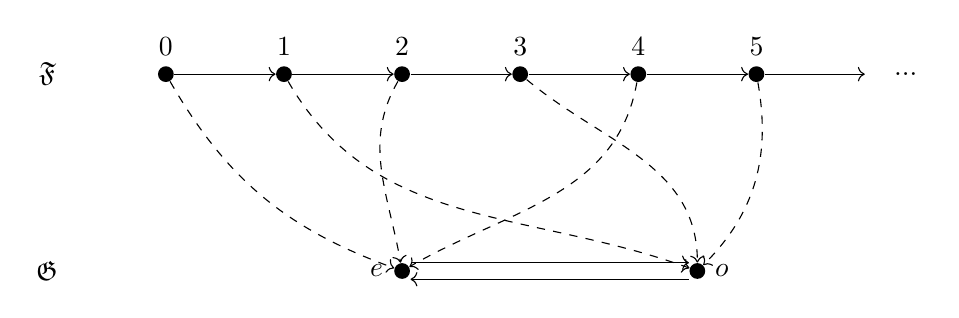
\begin{tikzpicture}
[n/.style={circle,fill=black,inner sep=0pt,minimum size=2mm}]
\node (f) at (-1.5,0) {$\fF$};
\node (g) at (-1.5,-2.5) {$\fG$};
\node[n] (0) at (0,0) {};
\node[n] (1) at (1.5,0) {};
\node[n] (2) at (3,0) {};
\node[n] (3) at (4.5,0) {};
\node[n] (4) at (6,0) {};
\node[n] (5) at (7.5,0) {};
\node (dot) at (9,0) {};
\node[above] at (0.north) {0};
\node[above] at (1.north) {1};
\node[above] at (2.north) {2};
\node[above] at (3.north) {3};
\node[above] at (4.north) {4};
\node[above] at (5.north) {5};
\node[right] at (dot.east) {$\dots$};
\node[n] (e) at (3,-2.5) {};
\node[n] (o) at (6.75,-2.5) {};
\node[left] at (e.west) {$e$};
\node[right] at (o.east) {$o$};
\draw[->,dashed] (0) to [out=300,in=160] (e);
\draw[->,dashed] (2) to [out=240,in=100] (e);
\draw[->,dashed] (4) to [out=-100,in=30] (e);
\draw[->,dashed] (1) to [out=-60,in=160] (o);
\draw[->,dashed] (3) to [out=-40,in=90] (o);
\draw[->,dashed] (5) to [out=-80,in=45] (o);
\draw[->] (0) -- (1);
\draw[->] (1) -- (2);
\draw[->] (2) -- (3);
\draw[->] (3) -- (4);
\draw[->] (4) -- (5);
\draw[->] (5) -- (dot);
\draw[->,transform canvas={yshift=3pt}] (e) -- (o);
\draw[->,transform canvas={yshift=-3pt}] (o) -- (e);
\end{tikzpicture}\end{center}
No property \(P\) is modally definable if \(\fF\) has \(P\) and \(\fG\)
lacks. This shows that there is no set of formulas characterizing the
asymmetric frames \(\forall(Rxy\to\neg Ryx)\)
\end{examplle}


\begin{corollary}[]
Let \(\tau\) be a modal similarity type, \(\fF\) a \(\tau\)-frame, and \(\phi\) a
\(\tau\)-formula. Then \(\fF\Vdash\phi\) if \(\ue\fF\Vdash\phi\)
\end{corollary}

\begin{proof}
Assume that \(\phi\) is not valid in \(\fF\). That is, there is a valuation \(V\)
and a state \(w\) s.t. \((\fF,V),w\Vdash\neg\phi\). By Proposition
\ref{prop2.59} \(\neg\phi\) is true at \(u_w\) in the ultrafilter extension of
\(\fM\). 
\end{proof}

We claim that every state has a reflexive successor \(\forall x\exists
   y(Rxy\wedge Ryy)\) is not modally definable, even though it is preserved
under taking disjoint unions, generated subframes and bounded morphic images.
Consider the frame in Example \ref{example2.58}.

\begin{theorem}[]
Let \(\tau\) be a modal similarity type, and \(\fF\) a \(\tau\)-frame. Then \(\fF\)
has an ultrapower \(\prod_U\fF\) s.t. \(\prod_U\fF\twoheadrightarrow\ue\fF\).
In a diagram
\begin{center}\begin{tikzcd}
\prod_U\fF\arrow[d, dash]\arrow[rd,two heads]\\
\fF&\ue\fF
\end{tikzcd}\end{center}
\end{theorem}

\begin{corollary}[]
Let \(\tau\) be a modal similarity type, and \(\phi\) a \(\tau\)-formula. If \(\phi\) defines a
first-order property of frames, then frame validity of \(\phi\) is preserved under
taking ultrafilter extensions
\end{corollary}

\begin{proof}
Let \(\phi\) be a modal formula which defines a first-order property of frames, and
let \(\fF\) be a frame s.t. \(\fF\Vdash\phi\). By the previous theorem, there
is an ultrapower \(\prod_U\fF\) of \(\fF\) s.t.
\(\prod_U\fF\twoheadrightarrow\ue\fF\). As first-order properties are
preserved under ultrapowers, \(\fF_U\fF\Vdash\phi\). But then \(\ue\fF\Vdash\phi\)
\end{proof}

\begin{theorem}[Goldblatt-Thomason Theorem]
Let \(\tau\) be a modal similarity type. A first-order definable class \(\sfK\) of
\(\tau\)-frames is modally definable iff it is closed under taking bounded
morphic images, generated subframes, disjoint unions and reflects ultrafilter extensions
\end{theorem}


\begin{exercise}
\label{ex3.3.2}
Consider the basic modal language. Show that the following properties of
frames are not modally definable
\begin{enumerate}
\item antisymmetry \((\forall xy)(Rxy\wedge Ryx\to x=y)\)
\item \(\abs{W}>23\)
\item \(\abs{W}<23\)
\item acyclicity
\item every state has at most one predecessor
\item every state has at least two successors
\end{enumerate}
\end{exercise}

\begin{proof}
\begin{enumerate}
\item Consider the frame in the example of bounded morphism
\item bounded morphism
\item Disjoint union
\item bounded morphism. Consider the following two frames: \(\fF=(\omega,S)\), the natural numbers with
the successor relation \(S=\{(n,m)\mid m=n+1\}\) and \par
\(\fG=(\{e,o\},\{(e,o),(o,e)\})\) as
\begin{center}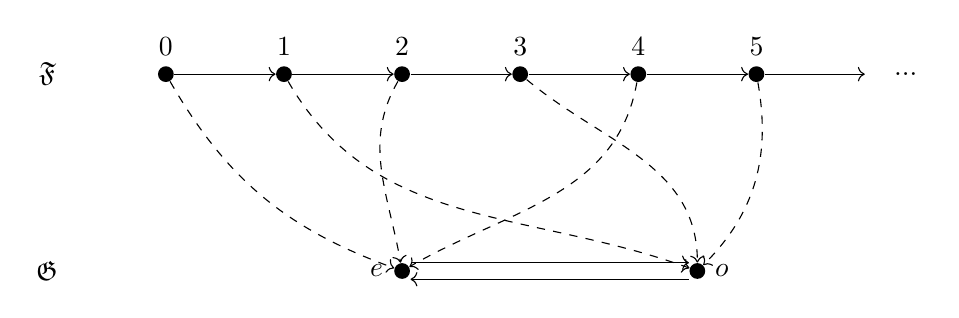
\begin{tikzpicture}
[n/.style={circle,fill=black,inner sep=0pt,minimum size=2mm}]
\node (f) at (-1.5,0) {$\fF$};
\node (g) at (-1.5,-2.5) {$\fG$};
\node[n] (0) at (0,0) {};
\node[n] (1) at (1.5,0) {};
\node[n] (2) at (3,0) {};
\node[n] (3) at (4.5,0) {};
\node[n] (4) at (6,0) {};
\node[n] (5) at (7.5,0) {};
\node (dot) at (9,0) {};
\node[above] at (0.north) {0};
\node[above] at (1.north) {1};
\node[above] at (2.north) {2};
\node[above] at (3.north) {3};
\node[above] at (4.north) {4};
\node[above] at (5.north) {5};
\node[right] at (dot.east) {$\dots$};
\node[n] (e) at (3,-2.5) {};
\node[n] (o) at (6.75,-2.5) {};
\node[left] at (e.west) {$e$};
\node[right] at (o.east) {$o$};
\draw[->,dashed] (0) to [out=300,in=160] (e);
\draw[->,dashed] (2) to [out=240,in=100] (e);
\draw[->,dashed] (4) to [out=-100,in=30] (e);
\draw[->,dashed] (1) to [out=-60,in=160] (o);
\draw[->,dashed] (3) to [out=-40,in=90] (o);
\draw[->,dashed] (5) to [out=-80,in=45] (o);
\draw[->] (0) -- (1);
\draw[->] (1) -- (2);
\draw[->] (2) -- (3);
\draw[->] (3) -- (4);
\draw[->] (4) -- (5);
\draw[->] (5) -- (dot);
\draw[->,transform canvas={yshift=3pt}] (e) -- (o);
\draw[->,transform canvas={yshift=-3pt}] (o) -- (e);
\end{tikzpicture}\end{center}

\item bounded morphism. Consider two frames \par
\(\fM=(\{a,b,c,d\},\{(a,c),(b,d)\})\) and
\(\fN=(\{a',b',c'\},\{(a',c'),(b',c')\})\) with surjective bounded
morphism
\(f(a)=a',f(b)=b',f(c)=f(d)=c'\). In \(\fM\) every state has at most one
predecessor, but not in \(\fN\)
\item bounded morphism. Consider two frames \par
\(\fM=(\{a,b,c\},\{(a,b),(a,c),(b,a),(b,c),(c,a),(c,b)\})\) and
\(\fN=(\{e\},\{(e,e)\})\) with bounded morphism \(f(a)=f(b)=f(c)=e\). In
\(\fM\), every state has two successors but in \(\fN\) there is only one
\end{enumerate}
\end{proof}

\subsection{Finite Frames}
\label{sec:orgca47886}
\subsubsection{Finite transitive frames}
\label{sec:orgf7357b2}
Let \(\fF=(W,R)\) be a point-generated finite transitive frame for the basic
modal similarity type, and let \(w\) be a root of \(\fF\). The Jankov-Fine
formula \(\phi_{\fF,w}\) is a description of \(\fF\) that has the following
property: it is satisfiable on a frame iff \(\fF\) is a bounded morphic
image of a generated subframe of \(\fG\)

We build Jankov-Fine formulas as follows. Enumerate the states of \(\fF\) as
\(w_0,\dots,w_n\), where \(w=w_0\). Associate each state \(w_i\) with a
distinct proposition letter \(p_i\). Let \(\phi_{\fF,w}\) be the conjunction
of the following formulas:
\begin{enumerate}
\item \(p_0\)
\item \(\Box(p_0\vee\dots\vee p_n)\)
\item \((p_i\to\neg p_j)\wedge\Box(p_i\to\neg p_j)\) for each \(i\neq j\le n\)
\item \((p_i\to\Diamond p_j)\wedge\Box(p_i\to\Diamond p_j)\) for each \(i,j\)
with \(Rw_iw_j\)
\item \((p_i\to\neg\Diamond p_j)\wedge\Box(p_i\to\neg\Diamond p_j)\) for each
\(i,j\) with \(\neg Rw_iw_j\)
\end{enumerate}


Note that as \(R\) is transitive, each node in \(\fF\) is accessible in one
step from \(w\). It followss that when formulas of the form
\(\psi\wedge\Box\psi\) are satisfied at \(w\) , \(\psi\) is true throughout \(\fF\).

\begin{lemma}[]
Let \(\fF\) be a trainsitive, finite, point-generated frame, let \(w\) be a
root of \(\fF\), and let \(\phi_{\fF,w}\) be the Jankov-Fine formula for
\(\fF\) and \(w\). Then for any transitive frame \(\fG\) we have the
following equivalence: there is a valuation \(V\) and a node \(v\) s.t.
\((\fG,V),v\Vdash\phi_{\fF,w}\) iff there exists a bounded morphism from
\(\fG_v\) onto \(\fF\)
\end{lemma}

\begin{proof}
Left to right. Suppose there is a valuation \(V\) and a node \(v\) s.t.
\((\fG,V),v\Vdash\phi_{\fF,w}\).  1 shows that \(v\in V(p_0)\). 2 and 3
shows that each of states satisfies exactly one of proposition letter
\(p_i\). Hence we build a function \(f:\fG_v\to\fF\) as \(f(v_i)=w_j\) if
\(v_i\in V(p_j)\) for each \(v_i\in\fG\). 2 and 3 show that this function is
well-defined.

Suppose \(R_{\fG}v_iv_j\) and \(\neg R_{\fF}w_iw_j\), then \((\fG,V),g\Vdash
    p_i\to\neg\Diamond p_j\) for all \(g\in\fG\). However, \((\fG,V),v_i\Vdash
    p_i\) and \((\fG,V),v_j\Vdash p_j\)

If \(R_{\fF}f(v_i)w_j\), then \((\fG,V),v_i\Vdash p_{f(v_i)}\to\Diamond
    p_j\). Hence there is a successor \(v_j\) of \(v_i\) s.t. \(f(v_j)=w_j\).
Therefore we find \(R_{\fG}v_iv_j\) and \(f\) is a bounded morphism

Right to left. Suppose there is a bounded morphism \(f\) from \(\fG_v\) onto
\(\fF\). Then clearly \(f(v)=w_0\). Let \(V(p_{f(v_i)})=\{v_j\mid f(v_j)=f(v_i)\}\) for all
\(v_i\in\fG\) . Then \((\fG,V),v\Vdash p_0\wedge\Box(p_0\vee\dots\vee p_n)
    \wedge(p_i\to\neg p_j)\wedge\Box(p_i\to\neg p_j)\).If \(R_{\fF}w_iw_j\) and
there is a \(v_i\in\fG\) s.t. \(f(v_i)=w_i\), then there is a \(f(v_j)=w_j\)
s.t. \(R_{\fG}v_iv_j\). Hence \((\fF,V),v\Vdash (p_i\to\Diamond
    p_j)\wedge\Box(p_i\to\Diamond p_j)\) for each \(i,j\) with \(Rw_iw_j\). 5 is
the same
\end{proof}

\begin{theorem}[]
Recall that \(\tau_0\) denotes the basic modal similarity type. Let \(\sfK\)
be a class of finite, transitive \(\tau_0\)-frames. Then \(\sfK\) is
definable within the class of finite, transitive \(\tau_0\)-frames iff it is
closed under taking (finite) disjoint unions, generated subframes and
bounded morphic images
\end{theorem}

\begin{proof}
Assume that \(\sfK\) is a class of finite, transitive \(\tau_0\)-frames and
satisfies the stated closure conditions. Let \(\Lambda_{\sfK}\) be the logic
of \(\sfK\); that is, \(\Lambda_{\sfK}=\{\phi\mid\fF\Vdash\phi,\text{ for
    all }\fF\in\sfK\}\). We will show that \(\Lambda_{\sfK}\) defines \(\sfK\).
We need to show that if \(\fF\Vdash\Lambda_{\sfK}\), where \(\fF\) is finite
and transitive, then \(\fF\in\sfK\).

First suppose \(\fF\) is point-generated with root \(w\). Consider the
Jankov-Fine formula \(\phi_{\fF,w}\) for \(\fF\) and \(w\). Clearly
\(\phi_{\fF,w}\) is satisfiable in \(\fF\) at \(w\), so
\(\neg\phi_{\fF,w}\not\in\Lambda_{\sfK}\). Hence there is some
\(\fG\in\sfK\) s.t. \(\fG\not\Vdash\neg\phi_{\fF,w}\); hence there is some
valuation \(V\) and state \(v\) s.t. \((\fG,V),v\Vdash\phi_{\fF,w}\). Thus
by the previous lemma, \(\fF\) is a bounded morphic image of the
point-generated subframe \(\fG_v\) of \(\fG\). By the closure condition on
\(\sfK\), it follows that \(\fF\in\sfK\).

Suppose that \(\fF\) is not point-generated. But then as
\(\fF\Vdash\Lambda_{\sfK}\), so does each point-generated subframe of
\(\fF\), hence all these subframes belongs to \(\sfK\). \(\fF\) is a bounded
morphic image of the disjoint union of its rooted generated subfrmaes,
\end{proof}
\subsubsection{The finite frame property}
\label{sec:org5d3a0ad}

\begin{definition}[]
A normal modal logic \(\Lambda\) has the finite model property w.r.t. some class of
models \(\sfM\) if \(\sfM\Vdash\Lambda\) and every formula \textbf{not} in \(\Lambda\) is
refuted in a \textbf{finite} model \(\fM\) in \(\sfM\). \(\Lambda\) has the finite model
property if it has the finite model property w.r.t. some class of models
\end{definition}

Informally, if a normal modal logic has the finite model property, it has a finite
semantic characterization: \textbf{it is precisely the set of formulas that some collection of}
\textbf{finite models makes globally true}

\begin{definition}[Finite Frame Property]
Let \(\Lambda\) be a normal modal logic and \(\sfF\) a class of finite frames. We say
\(\Lambda\) has the \textbf{finite frame property w.r.t.} \(\sfF\) if and only if
\(\sfF\Vdash\Lambda\), and for every formula \(\phi\) s.t. \(\phi\not\in\Lambda\)
there is some \(\fF\in\sfF\) s.t. \(\phi\) is falsifiable on \(\fF\). We say \(\Lambda\) has
the \textbf{finite frame property} iff it has the finite frame property w.r.t. some
class of finite frames
\end{definition}

\begin{definition}[Definable Variant]
Let \(\fM=(W,R,V)\) be a model and \(U\subseteq W\). We say \(U\) is
\textbf{definable in} \(\fM\) iff there is a formula \(\phi_U\) s.t. for all states
\(w\in W\), \(\fM,w\Vdash\phi_U\) iff \(w\in U\)

Any model \(\fM'\) based on the frame \((W,R)\) is called a \textbf{variant} of
\(\fM\). A variant \((W,R,V')\) of \(\fM\) is \textbf{definable in} \(\fM\) iff for
all proposition symbols \(p\), \(V'(p)\) is definable in \(\fM\). If \(\fM'\)
is a variant of \(\fM\) that is definable in \(\fM\), we call \(\fM'\) a
\textbf{definable variant} of \(\fM\)
\end{definition}

\begin{lemma}[]
Let \(\fM=(\fF,V)\) be a model and \(\fM'=(\fF,V')\) be a definable variant
of \(\fM\). For any formula \(\phi\), let \(\phi'\) be the result of uniformly
replacing each atomic symbol \(p\) in \(\phi\) by \(\phi_{V'(p)}\), where
\(\phi_{V'(p)}\) defines \(V'(p)\) in \(\fM\). Then for all formulas \(\phi\), and
all normal modal logics \(\Lambda\):
\begin{enumerate}
\item \(\fM',w\Vdash\phi\) iff \(\fM,w\Vdash\phi'\)
\item If every substitution instance of \(\phi\) is true in \(\fM\), then every
substitution instance of \(\phi\) is true in \(\fM'\)
\item If \(\fM\Vdash\Lambda\) then \(\fM'\Vdash\Lambda\)
\end{enumerate}
\end{lemma}

\begin{proof}
\begin{enumerate}
\item Induction on \(\phi\). For the base case we have \(\fM',w\Vdash p\) iff
\(\fM,w\Vdash\phi_{V'(p)}\). And
\((\neg\phi)'=\neg\phi'\),\((\phi\vee\psi)' =\phi'\vee\psi'\), and
\((\Diamond\phi)' =\Diamond\phi'\)
\item Let \(\psi\) be a substitution instance of \(\phi\) and suppose that
\(\fM'\not\Vdash\psi\). Thus there is some \(w\) in \(\fM\) s.t.
\(\fM',w\not\Vdash\psi\). By 1, this means \(\fM,w\not\Vdash\psi'\),
which means that \(\fM\not\Vdash\psi'\). But as \(\psi'\) is a
substitution instance of \(\psi\) and \(\psi\) is a substitution instance of \(\phi\), we have
that \(\psi'\) is a substitution instance of \(\phi\)
\item Normal modal logic are closed under uniform substitution
\end{enumerate}
\end{proof}

\begin{definition}[Distinguishing Model]
A model \(\fM\) is \textbf{distinguishing} if the relation \(\leftrightsquigarrow\)
of modal equivalence between states of \(\fM\) is the identity relation
\end{definition}

\begin{lemma}[]
\label{lemma2.37}
Let \(\fM=(\fF,V)\) be a a fintie distinguishing model. Then
\begin{enumerate}
\item For every state \(w\) in \(\fM\) there is a formula \(\phi_w\) that is
true at and only at \(w\)
\item \(\fM\) can define any subsets of \(\fF\). Hence \(\fM\) can define all
its variants
\item If \(\fM\Vdash\phi\) then \(\fF\Vdash\phi\)
\end{enumerate}
\end{lemma}

\begin{proof}
\begin{enumerate}
\setcounter{enumi}{2}
\item Suppose \(\fM\Vdash\phi\), then we have \(\fM'\Vdash\phi\) for some
definable variant of \(\fM\).
\end{enumerate}
\end{proof}

\begin{theorem}[]
A normal modal logic has the finite frame property iff it has the finite
model property
\end{theorem}


\begin{proof}
Suppose that \(\Lambda\) is a normal modal logic with the finite model property. and
assume that \(\Lambda\subset Form(\tau,\Phi)\)

Take a formula in the language \(ML(\tau,\Phi)\) that does not belong to \(\Lambda\). We
will show that \(\phi\) can be refuted on a finite frame \(\fF\) s.t.
\(\fF\Vdash\Lambda\)

As \(\Lambda\) has the finite model property, there is a finite model \(\fM\) s.t.
\(\fM\Vdash\Lambda\) and \(\fM,w\not\Vdash\phi\) for some state \(w\) \(\in\)
\(\fM\). Let \(\Sigma\) be the set of all subformulas of formulas in
\(\{\phi\}\cup\Lambda\) and let \(\fM^f\) be any filtration of \(\fM\)
through \(\Sigma\). As \(\fM\) is finite, so is \(\fM^f\). As \(\fM^f\) is a
filtration, it is a distinguishing model. By the Filtration Theorem
\ref{thm2.39}, \(\fM^f,\abs{w}\not\Vdash\phi\). Moreover
\(\fM^f\Vdash\Lambda\). Let \(\fF\) be the (finite) frame underlying
\(\fM^f\). By Lemma \ref{3.27} \(\fF\Vdash\Lambda\)
\end{proof}

\begin{exercise}
\label{ex3.4.1}
Let \(\fF\) be a trainsitive, finite, point-generated frame, let \(w\) be a
root of \(\fF\), and let \(\phi_{\fF,w}\) be the Jankov-Fine formula for
\(\fF\) and \(w\). Then for any transitive frame \(\fG\) we have the
following equivalence: there is a valuation \(V\) and a node \(v\) s.t.
\((\fG,V),v\Vdash\phi_{\fF,w}\) iff there exists a bounded morphism from
\(\fG_v\) onto \(\fF\)
\end{exercise}

\begin{proof}
Left to right. Suppose there is a valuation \(V\) and a node \(v\) s.t.
\((\fG,V),v\Vdash\phi_{\fF,w}\).  1 shows that \(v\in V(p_0)\). 2 and 3
shows that each of states satisfies exactly one of proposition letter
\(p_i\). Hence we build a function \(f:\fG_v\to\fF\) as \(f(v_i)=w_j\) if
\(v_i\in V(p_j)\) for each \(v_i\in\fG\). 2 and 3 show that this function is
well-defined.

Suppose \(R_{\fG}v_iv_j\) and \(\neg R_{\fF}w_iw_j\), then \((\fG,V),g\Vdash
    p_i\to\neg\Diamond p_j\) for all \(g\in\fG\). However, \((\fG,V),v_i\Vdash
    p_i\) and \((\fG,V),v_j\Vdash p_j\)

If \(R_{\fF}f(v_i)w_j\), then \((\fG,V),v_i\Vdash p_{f(v_i)}\to\Diamond
    p_j\). Hence there is a successor \(v_j\) of \(v_i\) s.t. \(f(v_j)=w_j\).
Therefore we find \(R_{\fG}v_iv_j\) and \(f\) is a bounded morphism

Right to left. Suppose there is a bounded morphism \(f\) from \(\fG_v\) onto
\(\fF\). Then clearly \(f(v)=w_0\). Let \(V(p_{f(v_i)})=\{v_j\mid f(v_j)=f(v_i)\}\) for all
\(v_i\in\fG\) . Then \((\fG,V),v\Vdash p_0\wedge\Box(p_0\vee\dots\vee p_n)
    \wedge(p_i\to\neg p_j)\wedge\Box(p_i\to\neg p_j)\).If \(R_{\fF}w_iw_j\) and
there is a \(v_i\in\fG\) s.t. \(f(v_i)=w_i\), then there is a \(f(v_j)=w_j\)
s.t. \(R_{\fG}v_iv_j\). Hence \((\fF,V),v\Vdash (p_i\to\Diamond
    p_j)\wedge\Box(p_i\to\Diamond p_j)\) for each \(i,j\) with \(Rw_iw_j\). 5 is
the same
\end{proof}

\begin{exercise}
\label{ex3.4.2}
Let \(\fM\) be a model, let \(\fM^f\) be any filtration of \(\fM\) through
some finite set of formulas \(\Sigma\), and let \(f\) be the natural map associated
with the filtration. If \(u\) is a point in the filtration, show that
\(f^{-1}[u]\) is definable in \(\fM\)
\end{exercise}

\begin{proof}
\(f^{-1}[u]=\{w\mid w\leftrightsquigarrow_\Sigma u\}\). Since \(\fM^f\) is
distinguishing, there is a formula \(\phi_u\) that is true at, and only at,
\(u\). Then \(\fM,w\Vdash\phi_u\) iff \(w\in f^{-1}[u]\)
\end{proof}
\section{Completeness}
\label{sec:org1643886}
\subsection{Preliminaries}
\label{sec:orge4e9b5f}
\begin{definition}[Modal Logics]
A \textbf{modal logic} \(\Lambda\) is a set of modal formulas that contains all
propositional tautologies and is closed under \textbf{modus ponens} and \textbf{uniform
substitution}. If \(\phi\in\Lambda\) we say that \(\phi\) is a \textbf{theorem} of \(\Lambda\) and write
\(\vdash_\Lambda\phi\). If \(\Lambda_1\) and \(\Lambda_2\) are modal logics
s.t. \(\Lambda_1\subseteq\Lambda_2\), we say that \(\Lambda_2\) is an
\textbf{extension} of \(\Lambda_1\)
\end{definition}

\begin{examplle}[]
\begin{enumerate}
\setcounter{enumi}{2}
\item Define \(\Lambda_{\sfS}\) be to \(\{\phi\mid\fG\Vdash\phi\text{, for
      all structures } \fG\in\sfS\}\), where \(\sfS\) is any class of frames or
any class of general frames. \(\Lambda_{\sfS}\) is a logic.
\setcounter{enumi}{3}
\item If \(\sfM\) is a class of models, then \(\Lambda_{\sfM}\) need \textbf{not} be
a logic. Consider a model \(\fM\) in which \(p\) is true at all nodes but
\(q\) is not. Then \(p\in\Lambda_{\fM}\) but \(q\not\in\Lambda_{\fM}\).
But \(q\) is obtainable from \(p\) by uniform substitution
\end{enumerate}
\end{examplle}

The logic generated by the empty set contains all the tautologies and nothing
else; we call it \(\PC\)

\begin{definition}[]
Let \(\psi_1,\dots,\psi_n,\phi\) be modal formulas. We say that \(\phi\) is
\textbf{deducible in propositional calculus from assumptions} \(\psi_1,\dots,\psi_n\)
if \((\psi_1\wedge\dots\wedge\psi_n)\to\phi\) is a tautology
\end{definition}

\begin{definition}[]
If \(\Gamma\cup\{\phi\}\) is a set of formulas then \(\phi\) \textbf{is deducible in \(\Lambda\) from}
\(\Gamma\) if \(\vdash_\Lambda\phi\) or there are formulas
\(\psi_1,\dots,\psi_n\in\Gamma\) s.t.
\begin{equation*}
\vdash_\Lambda(\psi_1\wedge\dots\wedge\psi_n)\to\phi
\end{equation*}
A set of formulas \(\Gamma\) is \textbf{\(\Lambda\)-consistent} if \(\Gamma\not\vdash_\Lambda\bot\).
\end{definition}

See more in \href{https://www.mv.helsinki.fi/home/negri/selected\_pub/dedthm.pdf}{Does the deduction theorem fail for modal logic?} and
\href{https://mathoverflow.net/questions/132268/deduction-theorem/132295}{MO discussion}

\begin{definition}[]
A modal logic \(\Lambda\) is \textbf{normal} if it contains the formulas
\begin{alignat*}{2}
&\text{(K)}&&\Box(p\to q)\to(\Box p\to\Box q)\\
&\text{(Dual)}\quad&&\Diamond\leftrightarrow\neg\Box\neg p
\end{alignat*}
and is closed under generalization (if \(\vdash_{\Lambda}\phi\) then \(\vdash_{\Lambda}\Box\phi\))
\end{definition}

\begin{lemma}[]
For any normal logic \(\Lambda\), if \(\vdash_\Lambda\phi\leftrightarrow\psi\) then
\(\vdash_\Lambda\Diamond\phi\leftrightarrow\Diamond\psi\)
\end{lemma}

The normal logic generated by the empty set is called \(\bK\). If \(\Gamma\) is a
non-empty set of formulas we usually denote the normal logic generated by \(\Gamma\)
by \(\bK\bGamma\)

\begin{alignat*}{2}
&(4)&&\Diamond\Diamond p\to\Diamond p\\
&(\text{T})&&p\to\Diamond p\\
&(\text{B})&&p\to\Box\Diamond p\\
&(\text{D})&&\Box p\to\Diamond p\\
&(\text{.3})&&\Diamond p\wedge\Diamond q\to
\Diamond(p\wedge\Diamond q)\vee\Diamond(p\wedge q)\vee\Diamond
(q\wedge \Diamond p)\\
&(\text{L})\quad&&\Box(\Box p\to p)\to\Box p
\end{alignat*}

\begin{center}
\begin{tabular}{ll}
\hline
\(\bK\) & the class of all frames\\
\(\KF\) & the class of transitive frames\\
\(\bT\) & the class of reflexive frames\\
\(\bB\) & the class of symmetric frames\\
\(\KD\) & the class of right-unbounded frames\\
\(\textbf{S4}\) & the class of reflexive, transitive frames\\
\(\textbf{S5}\) & the class of frames whose relation is an equivalence relation\\
\(\textbf{K4.3}\) & the class of transitive frames with no branching to the right\\
\(\textbf{S4.3}\) & the class of reflexive, transitive frames with no branching to the right\\
\(\KL\) & the class of finite transitive trees\\
\hline
\end{tabular}
\end{center}

A frame \((W,R)\) satisfying \(\forall x\forall y\forall z(Rxy\wedge Rxz\to
   (Ryz\vee y=z\vee Rzy))\) is said to have \textbf{no branching to the right}

\begin{definition}[Soundness]
Let \(\sfS\) be a class of frames. A normal modal logic \(\Lambda\) is \textbf{sound} w.r.t.
\(\sfS\) if \(\Lambda\subseteq\Lambda_{\sfS}\). (Equivalently: \(\Lambda\) is \textbf{sound}
w.r.t. \(\sfS\) if for all formulas \(\phi\), and all structures \(\fS\in\sfS\),
\(\vdash_\Lambda\phi\) implies \(\fS\Vdash\phi\)). If \(\Lambda\) is sound w.r.t.
\(\sfS\) we say that \(\sfS\) \textbf{is a class of frames for \(\Lambda\)}
\end{definition}


\index{strongly complete}
\begin{definition}[Completeness]
Let \(\sfS\) be a class of frames. A logic \(\Lambda\) is \textbf{strongly complete} w.r.t.
\(\sfS\) if for any set of formulas \(\Gamma\cup\{\phi\}\), if
\(\Gamma\Vdash_{\sfS}\phi\) then \(\Gamma\vdash_\Lambda\phi\).

A logic \(\Lambda\) is \textbf{weakly complete} w.r.t. \(\sfS\) if for any formula \(\phi\), if
\(\sfS\Vdash\phi\) then \(\vdash_\Lambda\phi\).
\end{definition}

A weakly complete w.r.t. \(\sfS\) if \(\Lambda_{\sfS}\subseteq\Lambda\). Thus
if we prove that a syntactically specified logic \(\Lambda\) is both sound and weakly
complete w.r.t. some class of structures \(\sfS\), we have \(\Lambda=\Lambda_{\sfS}\)

\begin{proposition}[]
\label{prop4.12}
A logic \(\Lambda\) is strongly complete w.r.t. a class of structures \(\sfS\) iff
every \(\Lambda\)-consistent set of formulas is satisfiable on some
\(\fS\in\sfS\). \(\Lambda\) is weakly complete w.r.t. a class of structures \(\sfS\)
iff every \(\Lambda\)-consistent formula is satisfiable on some \(\fS\in\sfS\)
\end{proposition}

\begin{proof}
Suppose \(\Lambda\) is not strongly complete w.r.t. \(\sfS\). There is a set of
formulas \(\Gamma\cup\{\phi\}\) s.t. \(\Gamma\Vdash_{\sfS}\phi\) but
\(\Gamma\not\vdash_\Lambda\phi\).  Then \(\Gamma\cup\{\neg\phi\}\) is
\(\Lambda\)-consistent but not satisfiable on any structure in \(\sfS\).

Suppose there is a \(\Lambda\)-consistent set \(\Gamma\) of formulas is not
satisfiable on all \(\fS\in\sfS\). Then \(\Gamma\Vdash_{\sfS}\phi\) is always true
\end{proof}

\begin{definition}[]
Assume we are working with a modal language of similarity type \(\tau\). A \textbf{modal
logic} in this language is a set of formulas containing all tautologies that
is closed under modus ponens and uniform substitution. A modal logic \(\Lambda\) is
\textbf{normal} if for every operator \(\triangledown\) it contains the axiom
\(\text{K}_{\triangledown}^i\) (for all \(i\) s.t. \(1\le
   i\le\rho(\triangledown)\)) and the axiom \(\text{Dual}_{\triangledown}\) and
is closed under the generalization rules
\begin{alignat*}{2}
&(\text{K}_{\triangledown}^i)&&
\triangledown(r_1,\dots,p\to q,\dots,r_{\rho(\triangledown)})\\
&&&\quad\to(\triangledown(r_1,\dots,p,\dots,r_{\rho(\triangledown)})
\to\triangledown(r_1,\dots,q,\dots,r_{\rho(\triangledown)}))\\
&(\text{Dual}_{\triangledown})&&\vartriangle(r_1,\dots,r_{\rho(\triangledown)})
\leftrightarrow\neg\triangledown(\neg r_1,\dots,\neg r_{\rho(\triangledown)})
\end{alignat*}
for a polyadic operator \(\triangledown\), generalization takes the following
form
\begin{equation*}
\vdash_{\Lambda}\sigma\text{ implies }\vdash_{\Lambda}\triangledown(\bot,\dots,\sigma,\dots,\bot)
\end{equation*}
\end{definition}

\begin{definition}[]
Let \(\tau\) be a modal similarity type. Given a set of \(\tau\)-formulas \(\Gamma\), we
define \(\bK_\tau\bGamma\), the normal modal logic \textbf{axiomatized} or \textbf{generated}
by \(\Gamma\), to be the smallest normal modal \(\tau\)-logic containing all formulas
in \(\Gamma\). Formulas in \(\Gamma\) are called \textbf{axioms} of this logic, and \(\Gamma\) may be called an
\textbf{axiomatization} of \(\bK_\tau\bGamma\)
\end{definition}


\subsection{Canonical Models}
\label{sec:orge0a7920}
\begin{definition}[$\Lambda$-MCSs]
A set of formulas \(\Gamma\) is \textbf{maximal \(\Lambda\)-consistent} if \(\Gamma\) is
\(\Lambda\)-consistent, and any set of formulas properly containing \(\Gamma\) is
\(\Lambda\)-inconsistent. We say its a \(\Lambda\)-MCS
\end{definition}

\begin{proposition}[Properties of MCSs]
\label{prop4.16}
If \(\Lambda\) is a logic and \(\Gamma\) is a \(\Lambda\)-MCS then
\begin{enumerate}
\item \(\Gamma\) is closed under modus ponens: if \(\phi,\phi\to\psi\in\Gamma\), then \(\psi\in\Gamma\)
\item \(\Lambda\subseteq\Gamma\)
\item for all formulas \(\phi\): \(\phi\in\Gamma\) or \(\neg\phi\in\Gamma\)
\item for all formulas \(\phi\),\(\psi\): \(\phi\vee\psi\in\Gamma\) iff \(\psi\in\Gamma\) or \(\phi\in\Gamma\)
\end{enumerate}
\end{proposition}

\begin{proposition}[Lindenbaum's Lemma]
If \(\Sigma\) is a \(\Lambda\)-consistent set of formulas then there is a
\(\Lambda\)-MCS \(\Sigma^+\) s.t. \(\Sigma\subseteq\Sigma^+\)
\end{proposition}

\begin{proof}
Let \(\phi_0,\phi_1,\dots\) be an enumeration of the formulas of our
language. We define the set \(\Sigma^+\) as the union of a chain of
\(\Lambda\)-consistent sets as follows:
\begin{align*}
\Sigma_0&=\Sigma\\
\Sigma_{n+1}&=
\begin{cases}
\Sigma_n\cup\{\phi_n\} &\text{ if this is $\Lambda$-consistent}\\
\Sigma_n\cup\{\neg\phi_n\}&\text{otherwise}
\end{cases}\\
\Sigma^+&=\bigcup_{n\ge0}\Sigma_n
\end{align*}
\begin{enumerate}
\item \(\Sigma_n\) is \(\Lambda\)-consistent, for all \(n\)
\item exactly one of \(\phi\) and \(\neg\phi\)is in \(\Sigma^+\)
\item if \(\Sigma^+\vdash_{\Lambda}\phi\), then \(\phi\in\Sigma^{+}\)
\item \(\Sigma^{+}\) is a \(\Lambda\)-MCS
\end{enumerate}
\end{proof}

\begin{definition}[]
The \textbf{canonical model} \(\fM^{\Lambda}\) for a normal modal logic \(\Lambda\) is the triple
\((W^\Lambda,R^\Lambda,V^\Lambda)\) where
\begin{enumerate}
\item \(W^\Lambda\) is the set of all \(\Lambda\)-MCSs
\item \(R^\Lambda\) is the binary relation on \(W^\Lambda\) defined by
\(R^\Lambda wu\) if for all formulas \(\psi\), \(\psi\in u\) implies \(\Diamond\psi\in
      w\). \(R^\Lambda\) is called the \textbf{canonical relation}
\item \(V^\Lambda\) is the valuation defined by \(V^\Lambda(p)=\{w\in W^\Lambda\mid
      p\in w\}\). \(V^\Lambda\) is called the \textbf{canonical valuation}
\end{enumerate}
\end{definition}

\begin{lemma}[]
\label{lemma4.19}
For any normal logic \(\Lambda\), \(R^\Lambda wv\) iff for all formulas \(\psi\), \(\Box\psi\in w\)
implies \(\psi\in v\)
\end{lemma}

\begin{proof}
Suppose \(R^\Lambda wv\) and \(\psi\not\in v\). As \(v\) is an MCS, \(\neg\psi\in
   v\). The \(\Diamond\neg\psi\in w\). As \(w\) is consistent,
\(\neg\Diamond\neg\psi\not\in w\). That is, \(\Box\psi\not\in w\)
\end{proof}

\begin{lemma}[Existence Lemma]
For any normal modal logic \(\Lambda\) and any state \(w\in W^\Lambda\), if
\(\Diamond\phi\in w\) then there is a state \(v\in W^\Lambda\) s.t.
\(R^\Lambda wv\) and \(\phi\in v\)
\end{lemma}

\begin{proof}
Suppose \(\Diamond\phi\in w\). Let \(v^-=\{\phi\}\cup\{\psi\mid\Box\psi\in
   w\}\). Then \(v^-\) is consistent. For suppose not. Then there are
\(\psi_1,\dots,\psi_n\) s.t.
\(\vdash_\Lambda(\psi_1\wedge\dots\wedge\psi_n)\to\neg\phi\), then we have
\(\vdash_\Lambda\Box(\psi_1\wedge\dots\wedge\psi_n)\to\Box\neg\phi\).  Also
as
\((\Box\psi_1\wedge\dots\wedge\Box\psi_n)\to\Box(\psi_1\wedge\dots\wedge\psi_n)\),
then we
\(\vdash_\Lambda(\Box\psi_1\wedge\dots\wedge\Box\psi_n)\to\Box\neg\phi\). Now
\(\Box\psi_1\wedge\dots\wedge\Box\psi_n\in w\) thus it follows that
\(\Box\neg\phi\in w\). Using dual, it follows that \(\neg\Diamond\phi\in w\),
which is impossible.

Let \(v\) be any MCS extending \(v^-\); such extensions exist by Lindenbaum's
Lemma. By construction \(\phi\in v\). Furthermore, for all formulas \(\psi\),
\(\Box\psi\in w\) implies \(\psi\in v\). Hence by Lemma \ref{lemma4.19},
\(R^\Lambda wv\)
\end{proof}

\begin{lemma}[Truth Lemma]
For any normal modal logic \(\Lambda\) and any formula \(\phi\), \(\fM^\Lambda,w\Vdash\phi\) iff
\(\phi\in w\)
\end{lemma}

\begin{proof}
Base case follows from the definition of \(V^\Lambda\). Boolean case from
Proposition \ref{prop4.16}.

\begin{alignat*}{3}
&\fM^\Lambda,w\Vdash\Diamond\phi\quad&&\Leftrightarrow
\quad&&\exists v(R^\Lambda wv\wedge\fM^\Lambda,v\Vdash\phi)\\
&&&\Leftrightarrow&&\exists v(R^\Lambda wv\wedge\phi\in v)\\
&&&\Rightarrow&&\Diamond\phi\in w
\end{alignat*}

Suppose \(\Diamond\phi\in w\), it suffices to find an MCS \(v\) s.t.
\(R^\Lambda wv\) and \(\phi\in v\), which is the existence lemma
\end{proof}

\begin{theorem}[Canonical Model Theorem]
Any normal modal logic is strongly complete w.r.t. its canonical model
\end{theorem}

\begin{proof}
Suppose \(\Sigma\) is a consistent set of the normal modal logic \(\Lambda\). By Lindenbaum's
Lemma there is a \(\Lambda\)-MCS \(\Sigma^+\) extending \(\Sigma\). By the previous lemma,
\(\fM^\Lambda,\Sigma^+\Vdash\Sigma\)
\end{proof}

\begin{theorem}[]
\(\bK\) is strongly complete w.r.t. to the class of all frames
\end{theorem}

\begin{proof}[]
By Proposition \ref{prop4.12}, to prove this result it suffices to find, for
any \(\bK\)-consistent set of formulas \(\Gamma\), a model \(\fM\) and a state \(w\)
in \(\fM\) s.t. \(\fM,w\Vdash\Gamma\). Simply choose \(\fM\) to be \((\fF^{\bK},V^{\bK})\)
\end{proof}


\subsection{Appications}
\label{sec:org8fd1713}
\begin{theorem}[]
The logic \(\textbf{K4}\) is strongly complete w.r.t. the class of transitive frames
\end{theorem}

\begin{proof}
Given a \(\KF\)-consistent set of formulas \(\Gamma\), it suffcies to find a model
\((\fF,V)\) and a state \(w\) in this model s.t.
\begin{enumerate}
\item \((\fF,V),w\Vdash\Gamma\) and
\item \(\fF\) is transitive
\end{enumerate}


\((W^{\KF},R^{\KF},V^{\KF}),\Gamma^+\Vdash\Gamma\). Suppose \(R^{\KF}wv\) and
\(R^{\KF}vu\). We wish to show that \(R^{\KF}wu\). Suppose \(\phi\in u\),
then \(\Diamond\phi\in v\), so \(\Diamond\Diamond\phi\in w\). But \(w\) is a
\(\KF\)-MCS, hence it contains \(\Diamond\Diamond\phi\to\Diamond\phi\)
\end{proof}

\begin{theorem}[]
\(\bT,\KB,\KD\) are strongly complete w.r.t. the classes of reflexive frames,
of symmetric frames, and of right-unbounded frames respectively
\end{theorem}


\begin{theorem}[]
\(\textbf{S4}\) is strongly complete w.r.t. the class of reflexive, transitive
frames. \(\textbf{S5}\) is strongly complete w.r.t. the class of frames whose
relation is an equivalence relation
\end{theorem}


\begin{definition}[Canonicity]
A formula \(\phi\) is \textbf{canonical} if for any normal logic \(\Lambda\), \(\phi\in\Lambda\)
implies that \(\phi\) is valid on the canonical frame for \(\Lambda\). A normal logic \(\Lambda\) is
\textbf{canonical} if its canonical frame is a frame for \(\Lambda\). (That is,
\(\Lambda\) is canonical if for all \(\phi\) s.t. \(\vdash_{\Lambda}\phi\), \(\phi\) is valid on the
canonical frame for \(\Lambda\) ) 
\end{definition}

\(\Lambda\) is strongly complete w.r.t. canonical 

4, T, B, D axioms are all canonical formulas.

\begin{definition}[Canonicity for a Property]
Let \(\phi\) be a formula, and \(P\) be a property. If the canonical frame for any
normal logic \(\Lambda\) containing \(\phi\) has property \(P\), then \(\phi\) is valid on any class
of frames with property \(P\), then \(\phi\) is \textbf{canonical for} \(P\).
\end{definition}

The class of all bidirectional frames is denoted by \(\sfF_t\), and a
bidirectional model is a model whose underlying frame belongs to \(\sfF_t\)

\begin{definition}[]
The minimal temporal logic \(\Lambda_{\sf_t}\) is \(\{\phi\mid \sfF_t\Vdash\phi\}\)
\end{definition}



\begin{definition}[]
A \textbf{normal temporal logic} \(\Lambda\) is a normal modal logic that contains \(p\to
   GPp\) and \(p\to HF p\). The smallest normal temporal logic is called
\(\bK_t\). We usually call normal temporal logics \textbf{tense logics}
\end{definition}

We want to show that \(\bK_t\) generated exactly the formulas in
\(\Lambda_{\sfF_t}\).

\begin{definition}[]
The canonical model for a tense logic \(\Lambda\) is the structure
\(\fM^\Lambda=(T^\Lambda,\{R_P^\Lambda,R_F^\Lambda\},V^\Lambda)\) where
\begin{enumerate}
\item \(T^\Lambda\) is the set of all \(\Lambda\)-MCSs
\item \(R_P^\Lambda\) is the binary relation on \(T^\Lambda\) defined by
\(R_P^\Lambda ts\) if for all formulas \(\phi\), \(\phi\in s\) implies \(P\phi\in t\)
\item \(R_F^\Lambda\) is the binary relation on \(T^\Lambda\) defined by
\(R_F^\Lambda ts\) if for all formulas \(\phi\), \(\phi\in s\) implies \(F\phi\in t\)
\item \(V^\Lambda\) is the valuation defined by \(V^\Lambda(p)=\{t\in T^\Lambda\mid
      p\in t\}\)
\end{enumerate}
\end{definition}

\begin{lemma}[]
\label{lemma4.35}
For any tense logic \(\Lambda\), if \(R_P^\Lambda ts\) then \(R_F^\Lambda st\) and if
\(R_F^\Lambda ts\) then \(R_P^\Lambda st\)
\end{lemma}

\begin{proof}
If \(R_P^\Lambda ts\) and suppose \(\phi\in t\). Then \(GP\phi \in t\). Hence
\(P\phi\in s\) and we have \(R_F^\Lambda st\)
\end{proof}

\begin{corollary}[]
\(\bK_t\) is strongly complete w.r.t. the class of all bidirectional frames,
and \(\bK_t=\Lambda_{\sfF_t}\)
\end{corollary}

\begin{proof}
\(\bK_t\) is strongly complete w.r.t. its canonical model. As we have just
seen, this model is based on a \emph{bidirectional} frame, so the strong frame
completeness result follows. Strong completeness implies weak completeness,
so \(\Lambda_{\sfF_t}\subseteq\bK_t\)
\end{proof}

\begin{definition}[]
A bidirectional frame \((T,R)\) is \textbf{dense} if there is a point between any two
related points (\(\forall xy(Rxy\to\exists z(Rxz\wedge Rzy))\)).
It is \textbf{right-unbounded} if every points has a successor.
\textbf{left-unbounded}. \textbf{unbounded} if both right- and left-unbounded. It is
\textbf{trichotomous} if any two points are equal or are related one way or the other
\((\forall xy(Rxy \vee x=y\vee Ryx))\) and a \textbf{weak total order} if it is both
transitive and trichotomous. We call a frame with all these properties a DUWTO-frame
\end{definition}

\begin{alignat*}{2}
&(4)&&FFp\to Fp\\
&(\text{D}_r)&&Gp\to Fp\\
&(\text{D}_l)\quad&&Hp\to Pp
\end{alignat*}
We obtain an unbounded canonical frame.

\begin{alignat*}{2}
&(den)\quad&& Fp\to FFp
\end{alignat*}

\begin{lemma}[]
\(Fp\to FFp\) is canonical for density
\end{lemma}

\begin{proof}
Let \(\Lambda\) be any tense logic containing \(Fp\to FFp\), let \((T^\Lambda,R^\Lambda)\) be its
canonical frame, and let \(t, t'\) be points in this frame s.t. \(R^\Lambda tt'\).
We have to show that there is a \(\Lambda\)-MCS \(s\) s.t. \(R^\Lambda ts\) and
\(R^\Lambda st'\). If we could show that
\(\{\phi\mid G\phi\in t\}\cup\{F\psi\mid \psi\in t'\}\) is consistent we
would have the desired result by Lemma \ref{lemma4.19} and \ref{lemma4.35}

So suppose for the sake of contradiction that this set is not consistent.
Then, for some finite set of formulas
\(\phi_1,\dots,\phi_m,\psi_1,\dots,\psi_n\) from this set
\begin{equation*}
\vdash_\Lambda(\phi_1\wedge\dots\wedge\phi_m\wedge F\psi_1\wedge\dots
\wedge F\psi_n)\to\bot
\end{equation*}
Define \(\widehat{\phi}\) to be \(\phi_1\wedge\dots\wedge\phi_m\) and
\(\widehat{\psi}\) to be \(\psi_1\wedge\dots\wedge\psi_n\). Note that
\(\widehat{\psi}\in t'\).

Now \(\vdash_\Lambda F\widehat{\psi}\to F\psi_1\wedge\dots\wedge F\psi_n\),
hence \(\vdash_\Lambda\widehat{\phi}\wedge F\widehat{\psi}\to\bot\), hence
\(\vdash_\Lambda\widehat{\phi}\to\neg F\widehat{\psi}\), and hence
\(\vdash_\Lambda G\widehat{\phi}\to G\neg F\widehat{\psi}\). Because
\(G\phi_1,\dots,G\phi_m\in t\), we have that \(G\widehat{\phi}\in t\) too, hence
\(G\neg F\widehat{\psi}\in t\), and hence \(\neg G\neg F\widehat{\psi}\not\in t\).
That is \(FF\widehat{\psi}\not\in t\). But this means that \(F\widehat{\psi}\not\in
   t\) as \(F\widehat{\psi}\to FF\widehat{\psi}\in t\). But now we have a
contradiction: as \(\widehat{\psi}\in t'\) and \(R^\Lambda tt'\), \(F\widehat{\psi}\in t\)
\end{proof}

\begin{alignat*}{2}
&(.3_r)&&(Fp\wedge Fq)\to F(p\wedge Fq)\vee F(p\wedge q)\vee F(q\wedge Fp)\\
&(.3_l)\quad&&(Pp\wedge Pq)\to P(p\wedge Pq)\vee P(p\wedge q)\vee P(q\wedge Pp)
\end{alignat*}
which is canonical for no-branching-to-the -left and -right respectively

\begin{proposition}[]
Any trichotomous frame \((T,R)\) is non-branching. Furthermore, if \(R\) is
transitive and non-branching and \(t\in T\), then the subframe of \((T,R)\)
generated by \(t\) is trichotomous
\end{proposition}

\begin{definition}[]
Let \(\KtQ\) be the smallest tense logic containing
4,\(\text{D}_l,\text{D}_r,den,.3_l\) and \(.3_r\)
\end{definition}

\begin{theorem}[]
\(\KtQ\) is strongly complete w.r.t. the class of DUWTO-frames
\end{theorem}

\begin{proof}
If \(\Gamma\) is a \(\KtQ\)-consistent set of formulas, extend it to a \(\KtQ\)-MCS
\(\Gamma^+\). Let \(\fM\) be the canonical model for \(\KtQ\) and let \(fG\) be
the submodel of \(\fM\) generated by \(\Gamma^+\). Then \(\fG,\Gamma^+\Vdash\Gamma\).
Moreover, the frame underlying \(\fG\) is a DUWTO-frame as required.
Conjunction of \(.3_l\) and \(.3_r\) is canonical for non-branching, \(\fM\)
is non-branching and \(\fG\) trichotomous
\end{proof}

\begin{theorem}[]
Every Sahlqvist formula is canonical for the first-order property it defines.
Hence given a set of Sahlqvist axioms \(\Sigma\), the logic \(\textbf{K\Sigma}\)
is strongly complete w.r.t. the class of frames \(\sf_\Sigma\)
\end{theorem}


\begin{exercise}
\label{ex4.3.1}
Let 1.1 be the axiom \(\Diamond p\to\Box p\). Show that \(\textbf{K1.1}\) is
sound and strongly complete w.r.t. the class of all frames \((W,R)\) s.t.
\(R\) is a partial function
\end{exercise}

\begin{proof}
Suppose \(\fF=(W,R)\) is a frame s.t. \(R\) is a partial function and
\(\fF\Vdash\Diamond p\). Then for an arbitrary valuation \(V\) and a point
\(w\), we have \((\fF,V),w\Vdash\Diamond p\). Then there is a point \(v\)
s.t. \(Rwv\) and \(v\in V(p)\). As \(R\) is a partial function, \(w\) has no
successor other than \(v\). Hence \((\fF,V),w\Vdash\Box p\). Hence
\(\fF\Vdash\Diamond p\to\Box p\).

Let \(\fM^C=(M^C,R^C,V^C)\) be the canonical model of \(\textbf{K1.1}\).
It suffices to prove \(R^C\) is a partial function. Suppose there are states
\(w,u,v\) s.t. \(R^Cwu\) and \(R^Cwv\). For any \(\phi\in u\),
\(\Diamond \phi\in w\) and \(\fM^C,w\Vdash\Diamond\phi\to\Box\phi\). Hence
\(\fM^C,w\Vdash\Box\phi\) and \(\phi\in v\) follows. Hence \(u\subseteq v\)
and \(v\subseteq u\) the same. So \(u=v\) and \(R\) is a partial function.
\end{proof}

\begin{exercise}
\label{ex4.3.2}
Let \(\Lambda\) be a normal temporal logic containing the axioms \(p\to GPp\) and
\(p\to HFp\). Show that if if \(R_P^\Lambda ts\) then \(R_F^\Lambda st\) and if
\(R_F^\Lambda ts\) then \(R_P^\Lambda st\)
\end{exercise}

\begin{proof}
   If \(R_P^\Lambda ts\) and suppose \(\phi\in t\). Then \(GP\phi \in t\). Hence
\(P\phi\in s\) and we have \(R_F^\Lambda st\)
\end{proof}

\begin{exercise}
\label{ex4.3.6}
Show that \(\textbf{S5}\) is complete w.r.t. the class of \textbf{globally related
frames}, that is, those frames \((W,R)\) where \(R\) connects any two points
\end{exercise}

\begin{proof}
Relation in canonical model of \(\textbf{S5}\) is equivalent. Given any
\(\textbf{S5}\)-consistent set of formulas \(\Gamma\),
\(\fM^{\textbf{S5}},\Gamma^+\Vdash\Gamma\). Consider the submodel \(\fG\) of canonical
model generated on \(\Gamma^+\), clearly \(\fG,\Gamma^+\Vdash\Gamma\). Obviously the
elements in \(\fG\) is the equivalence class of \(\Gamma^+\), hence the frame
underlying \(\fG\) is globally related.
\end{proof}

\begin{exercise}
\label{4.3.3}
Use canonical models to show that \(\textbf{K4.3}\) is strongly complete
w.r.t. the class of frames that are transitive and have no branching to the
right. Then, by proving suitable completeness results, show that the normal
logic axiomatized by 4 and \(\Box(p\wedge\Box p\to q)\vee\Box(q\wedge\Box
   q\to p)\) is \(\textbf{K4.3}\)
\end{exercise}

\begin{proof}
Let \(\fM^C=(W^C,R^C,V^C)\) be a canonical model of \(\textbf{K4.3}\). It
suffices to show that \(R^C\) is transitive and have no branching to the
right.
Suppose \(R^Cwv\) and \(R^Cwu\). 
\end{proof}
\subsection{Limitative Results}
\label{sec:org7271e25}
\(\KL\) is the normal modal logic generated by the Löb axiom \(\Box(\Box p\to
   p)\to\Box p\).

Every \textbf{canonical} logic is sound and strongly complete w.r.t. some class of frames
\begin{theorem}[]
\(\KL\) is not sound and strongly complete w.r.t. any class of frames, and
hence it is not canonical
\end{theorem}

\begin{proof}
Let \(\Gamma\) be \(\{\Diamond q_1\}\cup\{\Box(q_i\to\Diamond q_{i+1}\mid 1\le
   i\in\omega)\}\). We will show that \(\Gamma\) is \(\KL\)-consistent, and that no model
based on a \(\KL\)-frame can satisfy all formulas in \(\Gamma\) at a single point.

To show that \(\Gamma\) is consistent, it suffices to show that every finite subset \(\Psi\)
of \(\Gamma\) is consistent. Given any such \(\Psi\), for some natural number \(n\) there is
a finite set \(\Phi\) of the form \(\{\Diamond q_1\}\cup\{\Box(q_i\to\Diamond
   q_{i+1})\mid 1\le i<n\}\) s.t. \(\Psi\subseteq\Phi\subset\Gamma\). We show
that \(\Phi\), and hence \(\Psi\), is consistent.

Let \(\widehat{\Phi}\) be the conjunction of all the formulas in \(\Phi\). To show that
\(\widehat{\Phi}\) is \(\KL\)-consistent, it suffices to show that it can be
satisfied in a model based on a frame for \(\KL\), for this shows that
\(\neg\widehat{\Phi}\) is not valid on all frames for \(\KL\). Let \(\fF\) be
the frame consisting of \(\{0,\dots,n\}\) in their usual order; as this is a
transitive, converse well-founded frame by Example \ref{example3.9} it is a
frame for \(\KL\). Let \(\fM\) be any model based on \(\fF\) s.t. for all
\(1\le i\le n\), \(V(q_i)=\{i\}\). Then \(\fM,0\Vdash\widehat{\Phi}\) and
\(\widehat{\Phi}\) is \(\KL\)-consistent

Next, suppose that \(\KL\) is sound and strongly complete w.r.t. some class
of frames \(\sfF\); note that as \(\KL\) is not the inconsistent logic,
\(\sfF\) must be non-empty. Thus any \(\KL\)-consistent set of formulas can
be satisfied at some point in a model based on a frame in \(\sfF\). In
particular, there is \(\fM,w\Vdash\Gamma\). But this is impossible: because
\(\fM,w\Vdash\Gamma\) we inductively define an infinite path through \(\fM\)
starting at \(w\).
\end{proof}


\begin{remark}
A normal logic \(\Lambda\) is said to be \textbf{compact} when any \(\Lambda\)-consistent set \(\Sigma\)
can be satisfied in a frame for \(\Lambda\) at a single point.
\end{remark}

\begin{theorem}[]
\(\KL\) is weakly complete w.r.t. the class of all finite transitive trees
\end{theorem}

\begin{definition}[]
Let \(\Lambda\) be a normal modal logic. \(\Lambda\) is \textbf{(frame) complete} if there is a class of
frames \(\sfF\) s.t. \(\Lambda=\Lambda_{\sfF}\) and \textbf{(frame) incomplete}
\end{definition}

\(\KtTho\) is the tense logic generated by the following axioms
\begin{alignat*}{2}
&(.3_r)&&Fp\wedge Fq\to F(p\wedge Fq)\vee F(p\wedge q)\vee F(Fp\wedge q)\\
&(D_r)&&Gp\to Fp\\
&(L_l)&&H(Hp\to p)\to Hp
\end{alignat*}
The first two axioms are no branching to the right and right-unboundedness
respectively. The third is the Löb axiom written in terms of the backwards.
As all three axioms are valid on the natural numbers, \(\KtTho\) is
consistent. If \((T,R)\) is a frame for \(\KtTho\) and \(t\in T\), then
\(\{u\in T\mid Rtu\}\) is a right-unbounded strict total order

Let \(\KtThoM\) be the smallest tense logic containing \(\KtTho\) and the
McKinsey axiom \(GFp\to FGp\)

\begin{definition}[]
Let \((U,<)\) be a strict total order and \(S\subseteq U\). \(S\) is \textbf{cofinal
in} \(U\) if for every \(u\in U\) there is an \(s\in S\) s.t. \(u<s\)
\end{definition}

\begin{lemma}[]
Let \(\fF\) be any frame for \(\KtTho\). Then \(\fF\not\models GFp\to FGp\)
\end{lemma}

\begin{proof}
Let \(t\) be any point in \(\fF\), let \(U=\{u\in T\mid Rtu\}\) and let \(<\)
be the restriction of \(R\) to \(U\). As \(\fF\) validates all the \(\KtTho\)
axioms, \((U,<)\) is a right-unbounded strict order. Suppose we could show
that there is a non-empty proper subset \(S\) of \(U\) s.t. both \(S\) and
\(U\setminus S\) are cofinal in \(U\), then the lemma would be proved, for we
would merely need to define a valuation \(V\) on \(\fF\) s.t. \(V(p)=S\) and
\((\fF,V),t\not\Vdash GFp\to FGp\)

Take a cardinal \(\kappa\) that is larger than the size of \(U\). By ordinal
induction, we will define a sequence of pairs of sets
\((R_\alpha,S_\alpha)_{\alpha\le\kappa}\) s.t. \(R_\kappa\cap
   S_\kappa=\empty\) and both \(R_\kappa\) and \(S_\kappa\) are cofinal. We can
prove the lemma from this by taking \(S=S_\kappa\). The definition is as
follows
\begin{enumerate}
\item For \(\alpha=0\), take some points \(r_0\) and \(s_0\) in \(U\) s.t.
\(r_0<s_0\) and define \(R_0=\{r_0\}\) and \(S_0=\{s_0\}\)
\item If \(\alpha=\beta+1\)
\begin{enumerate}
\item if \(R_\beta\) or \(S_\beta\) is cofinal, then define
\(R_\alpha=R_\beta\) and \(S_\alpha=S_\beta\)
\item if neither \(R_\beta\) nor \(S_\beta\) is cofinal, then take some upper
bound \(r_\beta\) of \(S_\beta\) take some \(s_\beta\) bigger than
\(r_\beta\) and define \(R_\alpha=R_\beta\cup\{r_\beta\}\) and \(S_\alpha=S_\beta\cup\{s_\beta\}\)
\item If \(\alpha\) is a limit ordinal then define \(R_\alpha=\bigcup_{\beta<\alpha}R_\beta\)
and \(S_\alpha=\bigcup_{\beta<\alpha}S_\beta\)
\end{enumerate}
\end{enumerate}


It's easy to prove that \(R_\alpha\cap S_\alpha=\empty\) for every ordinal
\(\alpha\le\kappa\). If \(R_\kappa\) and \(S_\kappa\) were not cofinal, then
the map \(f:\kappa\to U\) given by \(f:\alpha\mapsto r_{\alpha+1}\) would be injective
\end{proof}

\begin{theorem}[]
\(\KtThoM\) is consistent and incomplete
\end{theorem}

\begin{proof}
Let \((\N,<)\) be the natural numbers in their usual order. Let \(A\) be the
collection of finite and co-finite subsets of \(\N\). \(A\) is closed under
boolean combinations and modal operations.
\end{proof}
\subsection{Transforming the Canonical Model}
\label{sec:org1da69f0}

\begin{figure}
\centering
\begin{subfigure}[b]{0.4\textwidth}
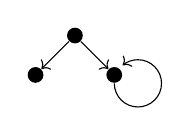
\begin{tikzpicture}
[n/.style={circle,fill=black,inner sep=0pt,minimum size=2mm}]
\node[n] (0) at (0,0) {};
\node[n] (1) at (-0.5,-0.5) {};
\node[n] (2) at (0.5,-0.5) {};
\draw[->] (2.south) arc (-180:130:3mm);
\draw[->] (0) -- (1);
\draw[->] (0) -- (2);
\end{tikzpicture}
\end{subfigure}
\begin{subfigure}[b]{0.4\textwidth}
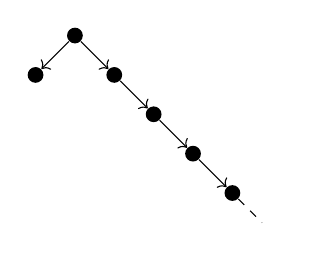
\begin{tikzpicture}
[n/.style={circle,fill=black,inner sep=0pt,minimum size=2mm}]
\node[n] (0) at (0,0) {};
\node[n] (1) at (-0.5,-0.5) {};
\node[n] (2) at (0.5,-0.5) {};
\node[n] (3) at (1,-1) {};
\node[n] (4) at (1.5,-1.5) {};
\node[n] (5) at (2,-2) {};
\node[] (6) at (2.5,-2.5) {};
\draw[->] (0) -- (1);
\draw[->] (0) -- (2);
\draw[->] (2) -- (3);
\draw[->] (3) -- (4);
\draw[->] (4) -- (5);
\draw[dashed] (5) -- (6);
\end{tikzpicture}
\end{subfigure}
\caption{A model and its unraveling}
\end{figure}


\begin{definition}[Unraveling]
Let \((W,R)\) be a frame generated by some point \(w\in W\). The \textbf{unraveling}
of \((W,R)\) around \(w\) is the frame \((\vv{W},\vv{R})\) where
\begin{enumerate}
\item \(\vv{W}\) is the set of finite sequences \((w,w_1,\dots,w_n)\) s.t.
\(w_1,\dots,w_n\in W\) and \(Rww_1,\dots,Rw_{n-1}w_n\)
\item If \(\vv{s_1},\vv{s_2}\in\vv{W}\), then \(\vv{R}\vv{s_1}\vv{s_2}\) if
there is some \(v\in W\) s.t. \(\vv{s_1}+(v)=\vv{s_2}\) where + denotes
sequence concatenation
\end{enumerate}


\begin{equation*}
\vv{V}(p)=\{(w,w_1,\dots,w_n)\in\vv{W}\mid w_n\in V(p)\}
\end{equation*}
The model \(\vv{\fM}=(\vv{W},\vv{R},\vv{V})\)  is called the unraveling of
\(\fM\) around \(w\)
\end{definition}

Unraveling yields an irreflexive, intransitive and asymmetric frame.

\begin{lemma}[]
Let \(\vv{\fM}=(\vv{W},\vv{R},\vv{V})\) be the unraveling of \(\fM=(W,R,V)\)
around \(w\). Then \((W,R)\) is a bounded morphic image of
\((\vv{W},\vv{R})\), and \(\fM\) is a bounded morphic image of \(\vv{\fM}\)
\end{lemma}

\begin{proof}
Let \(f:\vv{W}\to W\) be defined by \(f(w,w_1,\dots,w_n)=w_n\). \(f\) is
surjective, has the back and forth properties.

If \(Rf(\vv{w})v\), then let \(\vv{v}=\vv{w}+(v)\). Hence \(Rf(\vv{w})f(\vv{v})\)
\end{proof}

\textbf{Any} satisfiable set of formulas is satisfiable on a (irreflexive,
intransitive and asymmetric) tree: for if a set of formulas is satisfiable,
it is satisfiable on a point-generated model, hence by unraveling we have the
result. It follows that \(\bK\) is (strongly) complete w.r.t. this class of models

Suppose we unravel \(\fM\) around some generating point \(w\) to obtain
\((\vv{W},\vv{R},\vv{V})\). Now consider the model
\(\fM^*=(\vv{W},R^*,\vv{V})\) where \(R^*\) is the reflexive closure of
\(\vv{R}\). Trivially \(\fM^*\) is an \(\textbf{S4}\) model. Moreover, as
\((\vv{W},\vv{R})\) is a tree, \((\vv{W},R^*)\) is an \emph{antisymmetry} frame.

\begin{lemma}[]
\label{lemma4.53}
Let \(\fM=(W,R,V)\) be a reflexive transitive model generated by some
\(w\in W\), and let \((\vv{W},\vv{R},\vv{V})\) be the unraveling of \(\fM\)
around \(w\). Let \(R^*\) be the reflexive transitive closure of \(\vv{R}\),
and define \(\fM^*\) to be \((\vv{W},R^*,\vv{V})\). Then \(\fM\) is a bounded
morphic image of \(\fM^*\)
\end{lemma}

\begin{proof}
Only need to check forth property
\end{proof}

\begin{theorem}[]
\(\textbf{S4}\) is strongly complete w.r.t. the class of partially ordered
reflexive and transitive trees
\end{theorem}

\begin{proof}
If \(\Sigma\) is an \(\textbf{S4}\)-consistent set of formulas, and \(\Sigma^+\) is an
\(\textbf{S4}\)-MCS extending \(\Sigma\), then \(\fM^{\textbf{S4}},\Sigma^+\Vdash\Sigma\).
Moreover, as the \(\textbf{S4}\) axioms are canonical, \(\fM^{\textbf{S4}}\)
is a reflexive transitive model. We now transform this model into the
required partial order in two steps

\emph{Step 1}. Let \(\fM^S\) be the submodel of \(\fM^{\textbf{S4}}\) generated by
\(\Sigma^+\). Clearly this is a reflexive, transitive, point-generated model

\emph{Step 2}. Let \(\fM^*=(\vv{W},R^*,\vv{V})\) be the reflexive transitive closure
of the unraveling of \(\fM^S\) around \(\Sigma^+\)

By Lemma \ref{lemma4.53} \(\fM^S\) is a bounded morphic image of \(\fM^*\)
under \(f\), hence for all sequences \(\vv{s}\in f^{-1}[\Sigma]\), we have \(\fM^*,\vv{s}\Vdash\Sigma\).
\end{proof}

\(\textbf{K}_t\textbf{4.3}\) the tense logic generated by 4, \(.3_l\) and \(.3_r\)

\begin{definition}[]
Let \((T,R)\) be a transitive frame. A \textbf{cluster} on \((T,R)\) is a subset \(C\)
of \(T\) that is a maximal equivalent relation under \(R\). A cluster is
\textbf{simple} if it consists of a single reflexive point and \textbf{proper} otherwise.
\end{definition}

\begin{theorem}[]
\(\textbf{K}_t\textbf{4.3}\) is strongly complete w.r.t. the class of strict
total orders.
\end{theorem}

\begin{proof}
Let \(\Sigma\) be a \(\textbf{K}_t\textbf{4.3}\)-consistent set of formulas; expand it
to a \(\textbf{K}_t\textbf{4.3}\)-MCS \(\Sigma\). Let \(\fM=(T,R,V)\) be a canonical
model of \(\textbf{K}_t\textbf{4.3}\). By the canonicity of the axioms,
\(\fM\) is transitive and non-branching. Let \(\fM^S=(S,R^S,V^S)\) be the
submodel of \(\fM\) generated by \(\Sigma^+\); \(\fM^S\) is a transitive and
trichotomous model s.t. \(\fM^S,\Sigma^+\Vdash\Sigma\). But \(\fM^S\) may contain
clusters, which we will bulldoze away

\emph{Step 1}. Index the clusters in \(\fM^S\) by some suitable set \(I\)

\emph{Step 2}. Define an arbitrary strict order \(<^I\) on each cluster \(C_i\)

\emph{Step 3}. Define \(C^\flat_i\) to be \(C_i\times\Z\)

\emph{Step 4}. Define \(B\), the set underlying the bulldozed model, to be
\begin{equation*}
S^-\cup\bigcup_{i\in I}C_i^\flat
\end{equation*}
where \(S^-\) is the set (\(S\setminus\bigcup_{i\in I}C_i\)) of points \emph{not}
belonging to any clusters

\emph{Step 5}. Define a mapping \(\beta:B\to S\) by \(\beta(b)=b\) if \(b\in S^-\); and
\(\beta(b)=s\) if \(b=(s,z)\)

\emph{Step 6}. Define an ordering \(<^b\) on \(B\) by \(b<^b b'\) iff
\begin{itemize}
\item \textbf{either} (\(b\in S^-\) or \(b'\in S^-\)) and \(\beta(b)R^S\beta(b')\)
\item \textbf{or} \(b=(s,z)\) and \(b'=(s',z')\) and
\begin{itemize}
\item \textbf{either} \(s\) and \(s'\) belong to distinct clusters and \(\beta(b)R^S\beta(b')\)
\item \textbf{or} \(s\) and \(s'\) belong to the same cluster and \(z<_{\Z} z'\)
\item \textbf{or} \(s\) and \(s'\) belong to the same cluster \(C_i\) and \(z=z'\) and
\(s<^i s'\)
\end{itemize}
\end{itemize}


\emph{Step 7}. Define a valuation \(V^b\) on \((B,<^b)\) by \(b\in V(p)\) iff
\(\beta(b)\in V^S(p)\)

\emph{Step 8}. Define \(\fM^B\), the \textbf{bulldozed model}, to be \((B,<^b,V^b)\)
\end{proof}

\begin{claim}
The mapping \(\beta\) is a surjective bounded morphism from \((B,<^b)\) to
\((S,R^S)\) and the model \(\fM^S\) is a bounded morphic image of \(\fM^B\)
under \(\beta\)
\end{claim}

\begin{proof}
   
\end{proof}

\begin{claim}
\((B,<^b)\) is a strict total order
\end{claim}
\subsection{Step by Step}
\label{sec:orgdc8b12b}
In what follows, consistency means \(\KtQ\)-consistency and
\(\fM^c=(T^c,R^c,V^c)\) is this logic's canonical model. Furthermore we fix a
maximal consistent set \(\Sigma\); the goal of our proof is  to construct a model
\(\fM=(T,<,V)\) for \(\Sigma\) s.t. \((T,<)\) is an ordering isomorphic to \((\Q,<)\)

\begin{definition}[]
A \textbf{network} is a triple \(\caln=(N,<,\nu)\) s.t. \(R\) is a binary relation on
the set \(N\), and \(\nu\) is a labeling function mapping each point in \(N\) to a
maximal consistent set
\end{definition}

\begin{definition}[]
A network \(\caln=(N,<,\nu)\) is \textbf{coherent} if it satisfies:
\begin{enumerate}
\item < is a strict total ordering
\item \(\nu(s)R^c\nu(t)\) for all \(s,t\in N\) s.t. \(s<t\)
\end{enumerate}


A \textbf{network for} \(\Sigma\) is a network s.t. \(\Sigma\) is the label set of some node
\end{definition}

2 is equivalent to the requirement that if \(s<t\) then \(F\phi\in\nu(s)\)
for all \(\phi\in\nu(t)\) and \(P\phi\in\nu(t)\) for all \(\phi\in\nu(s)\)

\begin{definition}[]
A network \(\caln=(N,<,\nu)\) is \textbf{saturated} if it satisfies
\begin{enumerate}
\item < is unbounded to the left and to the right
\item < is dense
\item \(\caln\) is modally saturated. That is, we demand that (F) if
\(F\psi\in\nu(s)\) for some \(s\in N\), then there is some \(t\in N\) s.t.
\(s<t\) and \(\psi\in\nu(t)\) and (P) if \(P\psi\in\nu(s)\) for some
\(s\in N\), then there is some \(t\in N\) s.t. \(t<s\) and
\(\psi\in\nu(t)\)
\end{enumerate}
\end{definition}

A network is \textbf{perfect} if its both coherent and saturated

\begin{definition}[]
Let \(\caln=(N,<,\nu)\) be a network. The frame \(\fF_{\caln}=(N,<)\) is called
the \textbf{underlying frame} of \(\caln\). The \textbf{induced valuation} \(V_{\caln}\) on
\(\fF\) is defined by \(V_{\caln}(p)=\{s\in N\mid p\in\nu(s)\}\). The
structure \(\fJ_{\caln}=(\fF_{\caln},V_{\caln})\) is the \textbf{induced model}
\end{definition}

\begin{lemma}[Truth Lemma]
\label{lemma4.61}
Let \(\caln\) be a countably infinite perfect network. Then for all formulas
\(\psi\), and all nodes \(s\) in \(N\),
\begin{equation*}
\fJ_{\caln},s\Vdash\psi \quad\text{ iff }\quad
\psi\in\nu(s)
\end{equation*}
Moreover, \(\fF_{\caln}\) is isomorphic to the ordering of the rational numbers
\end{lemma}

\begin{proof}
Base case is from definition. Boolean case is from MCS.
The coherency of \(\caln\) drives the left to right implication, and
saturation takes care of the other direction

The underlying frame of a perfect network must be a dense, unbounded, strict
total ordering. Hence if it's countably infinite, it must be isomorphic to
\((\Q,<)\) by Cantor's Theorem
\end{proof}

It follows from Lemma \ref{lemma4.61} that we have reduced the task of finding a
model for our MCS \(\Sigma\) to the quest for a countable, perfect network for \(\Sigma\).


\begin{definition}[]
Let \(\caln=(N,<,\nu)\) be a network. An \textbf{S1-defect} of \(\caln\) consists of a
node \(s\in N\) that  has no successor, or no predecessor; an \textbf{S2-defect} is a
pair \((s,t)\) of nodes for which there is no intermediate point. An
\textbf{S3-defect} consists of (F) a node \(s\) and a formula \(F\psi\in\nu(s)\) for
which there is no \(t\) in \(N\) s.t. \(s<t\) and \(\psi\in\nu(t)\) or (P) a
node \(s\) and a formula \(P\psi\in\nu(s)\) for which there is no \(t\) in
\(N\) s.t. \(t<s\) and \(\psi\in\nu(t)\)
\end{definition}

\begin{definition}[]
Let \(\caln_0=(N_0,<_0,\nu_0)\) and \(\caln_1=(N_1,<_1,\nu_1)\) be two
networks. We say that \(\caln_1\) \textbf{extends} \(\caln_0\) (notation
\(\caln_1\rhd\caln_0\)) if \(\fF_{\caln_0}\) is a subframe of
\(\fF_{\caln_1}\) and \(\nu_0\) agrees with \(\nu_1\) on \(N_0\)
\end{definition}

\begin{lemma}[Repair Lemma]
For any defect of a finite coherent network \(\caln\) there is a finite
coherent \(\caln'\rhd\caln\) lacking this defect
\end{lemma}

\begin{proof}
Let \(\caln=(N,<,\nu)\) be a finite, coherent network and assume that \(\caln\)
has some defect.

\emph{S1-defects}



\emph{S2-defects}

Assume that there are nodes \(s\) and \(t\) in \(N\) for which there is no
intermediate point. By coherence of \(\caln\), \(\nu(s)R^c\nu(t)\), and by
canonicity of the density axiom that there is some MCS \(\Gamma\) s.t.
\(\nu(s)R^c\Gamma R^c\nu(t)\). Hence take some \emph{new} node \(u\) and define
\(\caln'=(N',<',\nu')\) by
\begin{alignat*}{3}
&N'&&:=&&N\cup\{u\}\\
&<'&&:=&&<\cup\{(x,u)\mid x\le s\}\cup\{(u,x)\mid t\le x\}\\
&\nu'&&:=&&\nu\cup\{(u,\Gamma)\}
\end{alignat*}
Now we need to prove \(\caln'\) is coherent.

\emph{S3-defects}

We only treat the P-defects. Assume that there is a node \(s\) in \(N\) and a
formula \(P\psi\in\nu(s)\)  for which is no \(t\) in \(N\) s.t. \(t<s\) and \(\psi\in\nu(t)\)

Let \(m\) be the unique point in \(N\) s.t.
\begin{enumerate}
\item \((m,P\psi)\) is an S3-defect in \(\caln\)
\item for all \(w<m\), \((w,P\psi)\) is \emph{not} a defect.
\end{enumerate}


Such an \(m\) must exist (it is either \(s\) itself or one of the finitely
many points preceding \(s\)) and, we can repair \((m,P\psi)\) without
problems by simply inserting the new point \(s'\) immediately before \(m\)

Choose some new point \(s'\) and let \(\Psi\) be an MCS containing \(\psi\) s.t.
\(\Psi R^c \nu(m)\); such a \(\Psi\) exists by the Existence Lemma for normal logics.
Define \(\caln'=(N',<',\nu')\) as follows
\begin{alignat*}{3}
&N'&&:=&&N\cup\{s'\}\\
&<'&&:=&&<\cup\{(x,s')\mid x<m\}\cup\{(s',x)\mid m\le x\}\\
&\nu'&&:=&&f\cup\{(s',\Psi)\}
\end{alignat*}
It only remains to ensure that \(\caln'\) satisfies the second coherency
condition

Suppose \(x<s'\). By construction \(\nu(s')=\Psi R^c\nu(m)\), and by coherency
of \(\caln\), \(\nu(x)R^c\nu(m)\). But \(R^c\) is the canonical relation for
\(\KtQ\) - a relation with no branching to the left - hence either \(\Psi
   R^c\nu(x),\Psi=\nu(x)\) or \(\nu(x)R^c\Psi\). We claim that the first two
options are impossible. For if \(\Psi R^c\nu(x)\) then \(\psi\in\Psi\) would
imply that \(P\psi\in\nu(x)\) and this contradicts the minimality of \(m\)
\end{proof}

\begin{theorem}[]
\(\KtQ\) is strongly complete w.r.t. \((\Q,<)\)
\end{theorem}

\begin{proof}
Choose some set \(S=\{s_i\mid i\in\omega\}\) and enumerate the set of
potential defects.
\end{proof}
\subsection{Rules for the Undefinable}
\label{sec:orgab9bb15}
Irreflexivity, although not definable in basic modal languages, \textbf{can} be
characterized in an alternative sense:
\begin{center}
If a temporal formula \(\psi\) is satisfiable on an irreflexive frame, then for any
proposition letter \(p\) not occurring in \(\psi\), the conjunction \((\neg
   Pp\wedgep\wedge\neg Fp)\wedge\psi\) is also satisfiable on that frame
\end{center}
For if \(\fF,V,s\Vdash\psi\), then
\(\fF,V',s\Vdash(\neg Pp\wedge p\wedge\neg Fp)\wedge\psi\) where \(V'\) is
just like \(V\) except that it assigns the singleton \(\{s\}\) to \(p\).

Now by taking the contrapositive of the above statement, we turn it into a
proof rule

\begin{itemize}
\item [(IRR)] if \(\vdash(\neg Pp\wedge p\wedge\neg Fp)\to\phi\) then \(\vdash\phi\), provided
\(p\) doesn't occur in \(\phi\)
\end{itemize}

Note that on the class of strict total orders the formula
\((\neg P\phi\wedge\phi\wedge\neg F\phi)\) is true at some state \(s\) iff
\(s\) is the \textbf{only} state where \(\phi\) holds (we need trichotomy and transitivity to
ensure this). Call this formula \(name(\phi)\)

\begin{definition}[]
The logic \(\KtQ^+\) is obtained by adding to \(\KtQ\) the irreflexivity rule
IRR. In what follows, consistency means \(\KtQ^+\)-consistency,
\(\vdash\phi\) means that \(\phi\) is provable in \(\KtQ^+\), and so on. The
canonical model for \(\KtQ^+\) is denoted by \(\fM^c\), the canonical
relation by \(R^c\)
\end{definition}

\begin{definition}[]
A maximal consistent set is called \textbf{witnessing} if it contains a formula of the
form \(name(\phi)\)
\end{definition}

\begin{definition}[]
Let \(W\) be a set of maximal consistent sets of formulas. Define
\(\fM^c\vert_W\) to be the submodel of the canonical model induced by \(W\);
that is, \(\fM^c\vert_W=(W,R,V)\) where \(R\) is the relation \(R^c\)
restricted to \(W\), and \(V\) is the canonical relation restricted to \(W\)
\end{definition}

\begin{definition}[]
A set \(W\) of maximal consistent sets is called \textbf{diamond saturated} if it
satisfies the requirement that for each \(\Sigma\in W\) and each formula
\(F\psi\in\Gamma\) there is a set \(\Psi\in W\) s.t. \(\Sigma R^c\Psi\) and
\(\psi\in\Psi\), and the analogous condition holds for past formulas
\end{definition}


\begin{definition}[Truth Lemma]
Let \(W\) be a diamond saturated set of maximal consistent sets of formulas.
Then for any \(\Gamma\in W\) and any formula \(\phi\):
\begin{equation*}
\fM^c\vert_W,\Gamma\Vdash\phi \quad\text{ iff }\quad
\phi\in\Gamma
\end{equation*}
\end{definition}

\begin{proposition}[]
\label{prop4.71}
Let \(\xi\) be some consistent formula. Then there is a countable, diamond
saturated collection \(W\) of witnessing MCSs s.t. \(\xi\in\Xi\) for some
\(\Xi\in W\)
\end{proposition}

All this is done to ensure that in the limit we are dealing with a labeled
graph meeting the requirements that
\begin{enumerate}
\item the label set of each point is an MCS
\item each label set contains a witness
\item if a formula of the form \(F\phi\) (\(P\phi\)) belongs to the label set of
some node, then there is an edge connecting this node to another one
containing \(\phi\) in its label set.
\end{enumerate}


Finally \(W\) is defined as the range of this infinite labeling function

Approximations to \(W\) will be called \textbf{networks}: a network is a quadruple
\(\caln=(N,E,d,\Lambda)\) s.t. \((N,E)\) is a finite, undirected, connected and
acyclic graph; \(d\) is a direction function mapping each edge \((s,t)\) of
the graph to either \(R\)or its converse \(R^{\smallsmile}\); and \(\Lambda\)
is a label function mapping each node of \(N\) to a \emph{finite} set of formulas

We first want to formulate coherence conditions on networks and dfine the
notion of a defect of network w.r.t. its ideal, \(W\). Since we are working
in the basic temporal similarity type - that is, we have diamonds both for
looking along \(R\) and along \(R^\smallsmile\) - there is an obvious way of
describing the network, from each of its nodes. Let \(\caln=(N,E,d,\Lambda)\) be
some network, and let \(s\) and \(t\) be two adjacent nodes of \(\caln\). We
use the following notational conventions
\begin{equation*}
\la st\ra:=
\begin{cases}
F&\text{if }d(s,t)=R\\
P&\text{if }d(t,s)=R^\smallsmile
\end{cases}
\end{equation*}
Moreover, let \(E(s)\) denote the set of nodes adjacent to \(s\). Finally, we
let \(\lambda(s)\) denote the conjunction \(\bigwedge\Lambda(s)\). Define
\begin{align*}
\Delta(\caln,s)&\quad:=\quad\lambda(s)\wedge\bigwedge_{v\in E(s)}\la sv\ra\theta(\caln,v,s)\\
\theta(\caln,t,s)&\quad:=\quad\lambda(t)\wedge\bigwedge_{s\neq v\in E(t)}\la tv\ra\theta(\caln,v,t)
\end{align*}
In other words, \(\Delta(\caln,s)\) starts with a local description \(\lambda(s)\) of
\(s\) and then proceeds to its neighbors. For each neighbor \(v\),
\(\Delta(\caln,s)\) writes a function operator if \(d(s,v)=R\) and then starts to
describe the network after \(v\) by calling \(\theta\). \(\theta(\caln,v,s)\) first gives a
local description \(\lambda(v)\) of \(v\), an then recursively proceeds to the
neighbors of \(v\) - except for \(s\). The omission of \(s\), together with
the finiteness and acyclicity of the graph, ensures that we end up with a
finite formula

\begin{lemma}[]
For any network \(\caln\) and any two nodes \(s,t\) in \(\caln\),
\(\Delta(\caln,s)\) is consistent iff \(\Delta(\caln, t)\) is consistent
\end{lemma}

\begin{proof}
By the connectedness of \(\caln\) it is sufficient to prove the Lemma for
adjacent \(s\) and \(t\).

So suppose that \(s\) and \(t\) are adjacent; without loss of generality
assume that \(d(s,t)=R\). Since \(\caln\) is fixed it won't lead to confusion
if we abbreviate \(\Delta(\caln,x)\) by \(\Delta(x)\) and \(\theta(\caln,x,y)\) by
\(\theta(x,y)\). Then by definition, \(\Delta(s)\) is given by
\begin{align*}
\Delta(s)&=\lambda(s)\wedge\bigwedge_{u\in E(s)}\la su\ra\theta(u,s)\\
&=\lambda(s)\wedge F\theta(t,s)\wedge\bigwedge_{t\neq u\in E(s)}\la su\ra\theta(u,s)\\
&=F\theta(t,s)\wedge\theta(s,t)
\end{align*}
Likewise we can show that
\begin{equation*}
\Delta(t)=\theta(t,s)\wedge P\theta(s,t)
\end{equation*}
But it is a general property of any logic extending \(\bK_t\) that for any
two formulas \(\alpha\) and \(\beta\), \(F\alpha\wedge\beta\) is consistent iff \(\alpha\wedge
   P\beta\) is consistent
\end{proof}

We call a network \(\caln\) \textbf{coherent} if \(\Delta(\caln,s)\) is consistent for each
of its nodes.

A \textbf{defect} of a network is either
\begin{enumerate}
\item a pair \((s,\phi)\) s.t. neither \(\phi\) nor \(\neg\phi\) belongs to \(\Lambda(s)\)
\item a pair \((s,F\phi)\) s.t.  \(F\phi\in\Lambda(s)\) while there is no
witness for this in the sense that \(\phi\in\Lambda(t)\) for some node
\(t\) with \(Est\) and \(d(s,t)=R\)
\item a similar pair \((s,P\phi)\)
\item a node \(s\) without a name; that is, \(name(\phi)\in\Lambda(s)\) for no formula
\end{enumerate}


A network \(\caln'\) \textbf{extends} a network \(\caln\) (\(\caln'\rhd\caln\)) if
\(N\subseeq N'\) while \(E=E'\cap N\times N,d=d'\vert_N\) and
\(\Lambda(s)\subseteq\Lambda'(s)\) for each node \(\caln\)

\begin{lemma}[]
For any defect of a finite coherent network \(\caln\) there is a finite,
coherent \(\caln'\rhd\caln\) lacking this defect
\end{lemma}

\begin{proof}
\emph{D4-defects}

If \(\Delta(\caln,s)\) is consistent, then there is a propositional variable
\(p\) that doesn't occur in any of the label sets. And we use the IRR-rule to
show that the formula \(\Delta(\caln,s)\wedge name(p)\) is consistent
\end{proof}

Now we return to the proof of Proposition \ref{prop4.71}
\begin{proof}
By a standard step-by-step construction we can define a sequence
\((\caln_i)_{i\in\N}\) of networks s.t.
\begin{enumerate}
\item \(\caln_0\) is a one-node network with label set \(\{\xi\}\)
\item \(\caln_j\) extends \(\caln_i\) whenever \(i<j\)
\item for every defect of any network \(\caln_i\) there is a network \(\caln_j\)
with \(j>i\) lacking this defect
\end{enumerate}


Let \(N\) be the set \(\bigcup_{i\in\N}N_i\); and for \(s\in N\), define
\(\Lambda(s)=\bigcup_{i\in\N}\Lambda_i(s)\). We claim that for every \(s\in N\),
\(\Lambda(s)\) is a witnessing MCS. Assume \(\Lambda(s)\) is not consistent; then there
are formulas \(\phi_1,\dots,\phi_n\) in \(\Lambda(s)\) s.t.
\(\phi_1\wedge\dots\wedge\phi_n\) is inconsistent. By construction, there
must be a \(k\in\N\) s.t. each \(\phi_i\) belongs to \(\Lambda_k(s)\). But
this contradicts the consistency of \(\Delta(\caln_k,s)\) and hence the coherency
of \(\caln_k\)

Finally define \(W\) as the range of \(\Lambda\). The preceding paragraphs show that
\(W\) is a collection of witnessing MCSs. By out definition of \(\caln_0\),
it follows that \(\xi\) belongs to some MCS in \(W\)

Now let \(F\phi\) be some formula in \(\Gamma\in W\). By definition, there is
some \(s\in N\) s.t. \(\Gamma=\Lambda(s)\), and thus, some \(i\in\N\) s.t.
\(F\phi\in\Lambda_i(s)\). By our construction there is some \(j\ge i\) and
some \(t\in N_j\) s.t. \(E_jst\) and \(\phi\in\Lambda_j(t)\). It follows that
\(\phi\in\Lambda(t)\), so it remains to prove that \(\Lambda(s)R^c\Lambda(t)\).
Suppose otherwise, then there is a formula \(\psi\in\Lambda(t)\) s.t.
\(F\psi\not\in\Lambda(s)\). Since \(\Lambda(s)\) is an MCS, this implies \(\neg
   F\psi\in\Lambda(s)\). Now let \(k\in\N\) be large enough that
\(\psi\in\Lambda_k(t)\) and \(\neg F\psi\in\Lambda_k(s)\). From this it is
immediate that \(\Delta(\caln_k,s)\) is inconsistent
\end{proof}

\begin{lemma}[]
Let \(W\) be a diamond saturated collection of witnessing maximal consistent
sets of formulas, and let < denote the canonical relation \(R^c\) restricted
to \(W\). Then the frame \((W,<)\) is a non-branching, unbounded, dense
strict ordering
\end{lemma}

\begin{proof}
Let \(W\) and \(<\) be as in the frame. \((W,<)\) is a subframe of the
canonical frame; hence it inherits every \textbf{universal} property of \(\fT\), such
as transitivity and non-branching. Irreflexivity follows from the fact that
\(\Gamma R^c\Gamma\) for no witnessing \(\Gamma\).

Unboundedness is not a universal condition. As \(F\top\) and \(P\top\) are
theorems of the logic and hence belong to every maximal consistent set

For density. Assume that \(\Gamma\) and \(\Delta\) are two MCSs s.t. \(\Gamma<\Delta\). We have to
find an MCS \(\Theta\) in \(W\) that lies between \(\Gamma\) and \(\Delta\). Let \(\delta\) be the formula s.t.
\(name(\delta)\in\Delta\). It follows from \(\Gamma<\Delta\) that
\(Fname(\delta)\in\Gamma\), so using the density axiom, we find that
\(FFname(\delta)\in\Gamma\). From this we may infer the existence of an MCS
\(\Theta\in W\) with \(\Gamma<\Tehta\) and \(Fname(\delta)\in\Theta\).

But is \(\Theta<\Delta\). Note that since < is non-branching to the right, we
already know that \(\Theta<\Delta\) or \(\Theta=\Delta\) or \(\Delta<\Theta\). But its
clear that \(F\delta\in\Theta\) and \(\neg F\delta\in\Delta\). Neither is it
possible that \(\Delta<\Theta\)for suppose otherwise. It would follows that
\(F\delta\in\Tehta\) that \(FF\delta\in\Delta\), so by transitivity axiom, \(F\delta\in\Delta\)
\end{proof}
\end{document}